\documentclass[Ingles]{assets/template/ic-tese-v3}
%\documentclass[Ingles,Final]{assets/template/ic-tese-v3}

\usepackage[latin1,utf8]{inputenc}

\usepackage[
    pdfauthor={Daniel De Lucca Fonseca},
    pdftitle={titulo},
    pdfkeywords={palavra-chave, palavra-chave},
    pdfproducer={Latex with hyperref},
    pdfcreator={pdflatex},
]{hyperref}

% Remover antes da versão final
\usepackage[
    draft,
%final,
]{changes}

\usepackage[printonlyused]{acronym}

\usepackage{amsmath}

\usepackage{listings}
\usepackage{xcolor}

\definecolor{codegray}{rgb}{0.5,0.5,0.5}
\definecolor{codeorange}{rgb}{0.8,0.3,0}
\definecolor{codeblue}{rgb}{0.2,0.2,0.6}

\lstdefinestyle{common}{
    basicstyle=\ttfamily\footnotesize,
    keywordstyle=\color{codeblue},
    commentstyle=\color{codegray}\itshape,
    stringstyle=\color{codeorange},
    showstringspaces=false,
    breaklines=true,
    frame=single,
    numbers=left,
    numberstyle=\tiny\color{codegray},
    captionpos=b,
    tabsize=2
}

\lstdefinestyle{pythonstyle}{
    style=common,
    language=Python
}

\lstdefinestyle{bashstyle}{
    style=common,
    language=bash,
    morekeywords={docker, echo, for, in, do, done, if, then, fi},
}

\begin{document}
    \autor{Daniel De Lucca Fonseca}
    \titulo{Título da Dissertação ou Tese em Português}
    \title{The Dissertation or Thesis Title in English or Spanish}
    \orientador{Prof. Dr. Edson Borin}
    \mestrado
    \datadadefesa{22}{04}{2025}

% Para a versão final defina:
%\avaliadorA{Prof. Dr. Primeiro Avaliador}{Instituição do primeiro avaliador}
%\avaliadorB{Profa. Dra. Segunda Avaliadora}{Instituição da segunda avaliadora}
%\avaliadorC{Dr. Terceiro Avaliador}{Instituição do terceiro avaliador}
%\avaliadorD{Prof. Dr. Quarto Avaliador}{Instituição do quarto avaliador}
%\avaliadorE{Prof. Dr. Quinto Avaliador}{Instituição do quinto avaliador}
%\avaliadorF{Prof. Dr. Sexto Avaliador}{Instituição do sexto avaliador}
%\avaliadorG{Prof. Dr. Sétimo Avaliador}{Instituição do sétimo avaliador}
%\avaliadorH{Prof. Dr. Oitavo Avaliador}{Instituição do oitavo avaliador}

% Para incluir a ficha catalográfica em PDF na versão final, descomente e ajuste:
%\fichacatalografica{arquivo.pdf}

    \paginasiniciais

    % Definição dos autores
\definechangesauthor[name={Edson Borin}, color=purple]{EB}
\definechangesauthor[name={Daniel Fonseca}, color=red]{DF}

% Borin (EB)
\newcommand{\EB}[1]{\comment[id=EB]{#1}} % Adiciona como comentário feito por EB
\newcommand{\EBH}[1]{\highlight[id=EB]{#1}} % Destaca o texto
\newcommand{\EBC}[2]{\EBH{#1} \comment[id=EB]{#2}} % Destaca e adiciona comentário
\newcommand{\EBADD}[1]{\added[id=EB]{#1}} % Adiciona texto
\newcommand{\EBRM}[1]{\deleted[id=EB]{#1}} % Remove texto
\newcommand{\EBRP}[2]{\replaced[id=EB]{#2}{#1}} % Substitui um texto pelo outro


% Edson's notes
% Daniel, mudei as macros por que não consegui adicionar comentários no rótulo de uma das tabelas com o modo anterior.
\renewcommand{\EB}[1]{{\textcolor{blue}{(EB: #1)}}}
\renewcommand{\EBH}[1]{{\hl{#1}}}
\renewcommand{\EBC}[2]{\EBH{#1}{\color{blue}(EB: #2)}}
\renewcommand{\EBADD}[1]{{\textcolor{blue}{#1}}}
\renewcommand{\EBRM}[1]{{\textcolor{lightgray}{(#1)}}}
\renewcommand{\EBRP}[2]{\EBRM{#1}\EBADD{#2}}
\newcommand{\EBRPD}[2]{#1 \EB{#1 $\rightarrow$ #2?}}

% Daniel (DF)
\newcommand{\DF}[1]{\comment[id=DF]{#1}} % Adiciona como coomentário feito por DF
\newcommand{\DFH}[1]{\highlight[id=DF]{#1}} % Destaca o texto
\newcommand{\DFC}[2]{\DFH{#1} \comment[id=DF]{#2}} % Destaca e adiciona comentário
\newcommand{\DFADD}[1]{\added[id=DF]{#1}} % Adiciona texto
\newcommand{\DFRM}[1]{\deleted[id=DF]{#1}} % Remove texto
\newcommand{\DFRP}[2]{\replaced[id=DF]{#2}{#1}} % Substitui um texto pelo outro
\newcommand{\DFTODO}[1]{\DFADD{TODO: #1}} % Adiciona um TODO com comentário
    \prefacesection{Dedicatória}
As dedicatórias devem ter apenas uma página.
\DFTODO{Escrever a dedicatória}
    \begin{epigrafe}{
    \it
    Vita brevis,\\
    ars longa,\\
    occasio praeceps,\\
    experimentum periculosum,\\
    iudicium difficile.\\
    \DFADD{Preciso fazer a epígrafe}
}

\hfill (Hippocrates)
\end{epigrafe}
    \prefacesection{Agradecimentos}
Os agradecimentos devem ocupar uma única página.
\DFTODO{Escrever os agradecimentos}
    % Sempre deve haver um resumo em português:
\begin{resumo}
    O resumo deve ter no máximo 500 palavras e deve ocupar uma única página.
    \DFTODO{Escrever o resumo}
\end{resumo}

\begin{abstract}
    The abstract must have at most 500 words and must fit in a single page.
    \DFTODO{Escrever o abstract}
\end{abstract}
    \prefacesection{List of Acronyms}

\begin{acronym}
    \acro{HPC}{High Performance Computing}
    \acro{GC}{Garbage Collector}
    \acro{COW}{Copy-On-Write}
    \acro{RSS}{Resident Set Size}
    \acro{VMS}{Virtual Memory System}
    \acro{UNICAMP}{Universidade Estadual de Campinas}
    \acro{GST3D}{Generalized S-transform in 3D}
    \acro{RAM}{Random Access Memory}
    \acro{OS}{Operating System}
    \acro{I/O}{Input/Output}
    \acro{CPU}{Central Processing Unit}
    \acro{API}{Application Programming Interface}
    \acro{macOS}{Macintosh Operating System}
    \acro{DDR4}{Double Data Rate 4}
    \acro{GB}{Gigabyte}
    \acro{GPU}{Graphics Processing Unit}
    \acro{3D}{Three-Dimensional}
\end{acronym}
    \prefacesection{List of Symbols}

\newcommand{\T}{$T$}
\newcommand{\Mpeak}{$M_{\text{peak}}$}
\newcommand{\Mt}{$M(t)$}

\begin{table}[h]
    \centering
    \begin{tabular}{|l|c|p{5cm}|}
        \hline
        \textbf{Symbol} & \textbf{Description}   & \textbf{Description}                                                                                                \\ \hline
        \T              & Execution Time         & A metric which represents the total time, measured in seconds, taken for the execution of a task.                   \\ \hline
        \Mpeak          & Peak Memory Usage      & A metric which denotes the highest memory consumption observed during the execution of a task, measured in \ac{MB}. \\ \hline
        \Mt             & Memory Usage over Time & A metric which eflects the continuous tracking of memory consumption as a function of time throughout the task.     \\ \hline
    \end{tabular}
    \caption{Summary of all symbols used in this thesis \EB{Talvez fique melhor deixar como lista em vez de tabela. Se preferir manter como tabela, mude o título da seção.}}
    \label{tab:summary-of-symbols}
\end{table}

    \listoffigures
    \listoftables

    \tableofcontents

    \fimdaspaginasiniciais

    \chapter{Introduction}
\label{ch:introduction}


\section{Motivation}
\label{sec:intro-motivation}

\DFTODO{Desafios no processamento de dados em larga escala, focando em sísmica}
\DFTODO{Problemas com o gerenciamento de recursos em sistemas distribuídos como o Dask}
\DFTODO{A necessidade de prever o consumo de memória para definir o tamanho do chunk em algoritmos que são memory-intensive}


\section{Objectives}
\label{sec:intro-objectives}

\DFTODO{Desenvolver um método para estimar o consumo de memória com a menor quantidade de execuções possíveis}
\DFTODO{Tornar o auto-chunking do Dask memory-aware para reduzir a tentativa e erro na alocação de recursos}


\section{Contributions}
\label{sec:intro-contributions}

\DFTODO{Criação de um modelo preditivo para o consumo de memória}
\DFTODO{Desenvolvimento de um método para estimar o consumo de memória com poucas execuções}
    \chapter{Fundamental Concepts}
\label{ch:fundamental-concepts}

\DFTODO{Definir os conceitos fundamentais que serão explicados}
    \chapter{Related Work}
\label{ch:related-work}

\DFTODO{Definir os trabalhos relacionados que serão discutidos neste capítulo}
    \chapter{Measuring Memory Consumption of Python Programs}
\label{ch:measuring-memory-consumption}
%
%
%\section{Introduction}
%\label{sec:mmc-introduction}
%
%Accurately measuring the memory consumption of Python programs is a fundamental aspect of performance analysis, especially in the context of scientific computing and data analysis workflows.
%Scientific applications often involve large-scale computations, high-dimensional datasets, and complex algorithms that necessitate the use of \ac{HPC} environments such as supercomputers and distributed systems.
%In these environments, resource allocation is a critical factor, directly impacting both computational efficiency and cost-effectiveness.
%Understanding the memory usage patterns of applications enables researchers and engineers to allocate appropriate resources, optimize computational workflows, and prevent system-level bottlenecks.
%
%In scientific workflows, the need for precise memory measurement extends beyond mere resource allocation.
%Memory profiling is instrumental in identifying inefficiencies, diagnosing performance issues, and ensuring the scalability of algorithms across diverse computational environments.
%Although this thesis primarily focuses on the execution of scientific workflows rather than their optimization, the accurate measurement of memory consumption remains pivotal.
%Without precise memory metrics, the evaluation of algorithmic performance and the reproducibility of experimental results can be significantly compromised.
%
%\subsection{Factors Affecting Memory Consumption Evaluation}
%\label{subsec:mmc-factors-affecting-memory-consumption-evaluation}
%
%The evaluation of memory consumption in Python applications is influenced by a multitude of factors spanning both the language's inherent characteristics and the underlying operating system's behavior.
%Python, as a high-level language, abstracts many low-level memory management operations, introducing complexities that can obscure the true memory footprint of an application.
%
%\begin{enumerate}
%    \item \textbf{Dynamic Memory Allocation}:
%    Python's memory model relies heavily on dynamic memory allocation, facilitated by its internal memory manager.
%    The interpreter frequently allocates and deallocates memory for objects, leveraging techniques such as reference counting and cyclic garbage collection.
%    These mechanisms introduce variability in memory usage, as memory may not be immediately released upon object deletion, leading to transient peaks in memory consumption.
%
%    \item \textbf{Garbage Collection}:
%    Python employs a \ac{GC} to manage memory, particularly for cyclic references that reference counting alone cannot handle.
%    The \ac{GC} operates in generational cycles, triggering collections based on thresholds related to object allocations and deallocations.
%    The timing of these collections can significantly affect memory profiling, as delayed garbage collection may artificially inflate memory usage metrics.
%
%    \item \textbf{Memory Fragmentation}:
%    Both Python's memory allocator (e.g., pymalloc~\cite{pymalloc}) and the underlying C libraries can cause memory fragmentation.
%    Fragmentation leads to inefficient memory utilization, where the allocated memory space cannot be fully utilized due to non-contiguous free blocks.
%    This phenomenon can result in higher apparent memory usage than the actual data footprint.
%
%    \item \textbf{Operating System Optimizations}:
%    Modern operating systems implement various memory management optimizations, such as virtual memory, \ac{COW}, and memory compression.
%    The virtual memory system abstracts physical memory, allowing processes to perceive a contiguous memory space.
%    \ac{COW} mechanisms, often triggered during process forking, can complicate memory measurements by deferring actual memory duplication until modification occurs.
%    Additionally, features like Linux's zswap~\cite{zswap} and zram~\cite{zram} compress memory pages to optimize \ac{RAM} usage, further obscuring accurate memory accounting.
%
%    \item \textbf{Caching Mechanisms}:
%    Python and the operating system both employ caching strategies that can skew memory usage metrics.
%    For instance, Python maintains internal caches for frequently used objects (e.g., small integers and strings), while the \ac{OS} uses disk and memory caches to optimize \ac{I/O} operations.
%    These caches can persist across program executions, leading to inconsistent memory profiles unless explicitly cleared.
%
%    \item \textbf{Third-Party Libraries}:
%    Scientific applications often rely on third-party libraries (e.g., NumPy~\cite{numpy}, pandas~\cite{pandas}, TensorFlow~\cite{tensorflow}), which may implement their own memory management strategies.
%    These libraries, typically written in C or C++, interact directly with system memory, bypassing Python's \ac{GC}.
%    Consequently, memory usage attributed to Python may not fully represent the actual consumption, necessitating specialized profiling tools to capture native allocations.
%\end{enumerate}
%
%\subsection{The Criticality of Precise Memory Measurement in Experiments}
%\label{subsec:mmc-criticality-of-precise-memory-measurement}
%
%Achieving precise memory measurement is a delicate and challenging task, particularly in experimental setups where even minor inconsistencies can introduce significant biases.
%Inaccurate memory profiling can lead to erroneous conclusions about an algorithm's efficiency, scalability, and resource requirements.
%
%One of the primary challenges is the accumulation of residual memory from previous executions.
%This issue is especially pronounced in interactive environments like Jupyter~\cite{jupyter} notebooks, where code cells can be executed multiple times without restarting the kernel.
%Each execution may leave behind allocated memory that is not immediately reclaimed, either due to lingering references or delayed garbage collection.
%This residual memory inflates subsequent memory usage measurements, creating misleading results.
%
%For example, consider a scenario where a data-intensive operation is repeatedly executed within a Jupyter notebook.
%Even if the data structures are explicitly deleted using \texttt{del}, Python's \ac{GC} might not immediately free the associated memory, particularly if a reference exist in the notebook's global namespace or within closures.
%Over time, this leads to cumulative memory bloat, distorting the true memory footprint of the operation.
%
%Beyond interactive environments, process-level memory accumulation can occur when running batch scripts or automated workflows.
%If multiple experiments are executed sequentially within the same process without proper memory isolation, residual allocations from earlier runs can affect subsequent measurements.
%Techniques such as spawning isolated subprocesses for each experiment can mitigate this issue, ensuring clean memory states between runs.
%
%Another critical consideration is the impact of measurement tools themselves.
%Profiling tools, whether external (e.g., psutil~\cite{psutil}, resource~\cite{importlib_resources}) or internal (e.g., tracemalloc~\cite{tracemalloc}), introduce overhead that can influence the very metrics they aim to capture.
%High-frequency sampling, for instance, increases \ac{CPU} and memory load, potentially skewing performance characteristics.
%Moreover, tools that rely on instrumentation may alter code execution paths, subtly affecting memory allocation patterns.
%
%To address these challenges, rigorous experimental protocols are essential.
%This includes:
%
%\begin{itemize}
%    \item Isolating experiments in separate processes or containers to prevent cross-contamination of memory states.
%    \item Resetting the environment (e.g., restarting the Python interpreter or Jupyter kernel) before each measurement to ensure a clean slate.
%    \item Controlling external factors, such as disabling \ac{OS}-level caches or running benchmarks on dedicated, idle systems to minimize background noise.
%    \item Using hybrid measurement techniques, combining high-level process metrics with low-level memory tracing for comprehensive profiling.
%\end{itemize}
%
%In conclusion, precise memory measurement is not merely a technical detail but a cornerstone of robust experimental methodology.
%It underpins the reliability and validity of performance evaluations, guiding both theoretical insights and practical optimizations in scientific computing.
%
%
%\section{Approaches to Measure Memory Consumption}
%\label{sec:mmc-approaches}
%
%When measuring memory consumption in Python programs, it is essential to distinguish between two broad categories of approaches: external measurement techniques and internal measurement techniques.
%This classification helps clarify the scope and effectiveness of different methods, as each group offers unique insights into memory usage from different perspectives.
%
%\begin{itemize}
%    \item \textbf{External Measurement Approaches} involve monitoring memory usage from outside the Python runtime environment.
%    These techniques interact directly with the operating system to gather data about process memory consumption.
%    They are particularly effective for capturing the overall memory footprint of a program, including memory allocated by external libraries, system-level resources, and native code executed alongside Python.
%    Examples include tools like psutil, the resource module, and accessing memory metrics from the Linux /proc~\cite{procfs} filesystem.
%
%    \item \textbf{Internal Measurement Approaches}, on the other hand, operate within the Python runtime itself.
%    These methods provide fine-grained visibility into Python-specific memory allocations, allowing developers to trace memory usage down to individual objects, code lines, or function calls.
%    They are invaluable for identifying memory leaks, inefficient data structures, and understanding memory behavior at a granular level.
%    The tracemalloc module is a prime example of an internal measurement approach.
%\end{itemize}
%
%The separation into these two categories is not arbitrary; it reflects the complementary nature of the information provided.
%External tools offer a high-level, system-wide view of memory consumption, which is crucial for understanding how a Python program interacts with the broader operating environment.
%In contrast, internal tools delve deep into Python’s memory management, offering detailed diagnostics that external tools cannot capture.
%
%Combining both external and internal measurement techniques often yields the most comprehensive understanding of a program’s memory behavior.
%External tools can detect overall memory growth trends and system resource usage, while internal tools can pinpoint the specific code responsible for memory allocation.
%This dual approach is especially useful in scientific computing workflows, where performance optimization requires both macro-level monitoring and micro-level diagnostics.
%
%\subsection{External Measurement Approaches}
%\label{subsec:mmc-external-measurement-approaches}
%
%\subsubsection{psutil}
%
%The psutil library is a cross-platform tool that allows Python programs to access system details and process information, including memory usage.
%It interacts with the operating system to retrieve real-time data about process memory, \ac{CPU} usage, and other system metrics.
%
%psutil works by interfacing with \ac{OS}-level \ac{API}, such as /proc on Linux, the Windows \ac{API} on Windows systems, and system calls on \ac{macOS}.
%It can report key memory metrics like:
%
%\begin{itemize}
%    \item \textbf{\ac{RSS}}:
%    The portion of memory occupied by a process that is held in \ac{RAM}.
%
%    \item \textbf{\ac{VMS}}:
%    The total amount of virtual memory used by the process.
%
%    \item \textbf{Shared Memory}:
%    Memory shared with other processes.
%\end{itemize}
%
%psutil provides a comprehensive overview of system-wide and process-specific resource usage, making it a versatile tool for performance monitoring.
%
%\subsubsection{resource Module}
%
%The resource module is part of Python's standard library and offers a lightweight method to track resource usage of the current process.
%It provides metrics such as maximum \ac{RSS}, which reflects the peak physical memory usage during the execution of the program.
%
%Unlike psutil which can monitor ongoing memory usage, resource is primarily used for capturing peak memory usage at specific checkpoints in the code.
%This makes it ideal for benchmarking and performance evaluations.
%
%\subsubsection{/proc Filesystem}
%
%On Linux systems, the /proc virtual filesystem provides detailed information about processes, including memory usage.
%Accessing \texttt{/proc/[pid]/smaps} allows for fine-grained analysis of memory allocation.
%
%The smaps file breaks down memory usage into categories such as:
%
%\begin{itemize}
%    \item \textbf{Private and Shared Memory}:
%    Differentiates between private memory and memory shared with other processes.
%
%    \item \textbf{Anonymous Pages}:
%    Memory not backed by any file.
%
%    \item \textbf{Heap and Stack Segments}:
%    Detailed insights into dynamic memory allocations.
%\end{itemize}
%
%While powerful, this approach requires root access for detailed process information and involves parsing raw text files, which can add complexity.
%
%\subsection{Internal Measurement Approaches}
%\label{subsec:mmc-internal-measurement-approaches}
%
%\subsubsection{tracemalloc}
%
%tracemalloc is a built-in Python module designed for tracing memory allocations.
%It hooks into Python's memory allocator to record the size and source of each allocation, capturing stack traces for memory usage hotspots.
%
%Key features of tracemalloc include:
%
%\begin{itemize}
%    \item \textbf{Memory Snapshots}:
%    Capturing snapshots of memory usage at different points in the program's execution.
%
%    \item \textbf{Snapshot Comparisons}:
%    Analyzing changes in memory usage between snapshots.
%
%    \item \textbf{Tracking Allocation Sources}:
%    Identifying the specific lines of code responsible for memory usage.
%
%    \item \textbf{Filtering and Grouping}:
%    Aggregating memory statistics based on filenames, line numbers, or function calls.
%\end{itemize}
%
%While tracemalloc introduces some overhead, its granularity makes it invaluable for debugging memory-related issues within Python applications.
%
%
%\section{Materials and Methods}
%\label{sec:mmc-materials-methods}
%
%\subsection{Experiment Setup}
%\label{subsec:mmc-experiment-setup}
%
%All experiments were conducted on Node 9 of the \ac{UNICAMP} Discovery Lab, a high-performance Linux machine configured with the following hardware specifications:
%
%\begin{itemize}
%    \item \textbf{\ac{CPU}}:
%    AMD Ryzen 7--5700X, featuring 8 physical cores and 16 logical threads.
%
%    \item \textbf{Memory}:
%    32 GB \ac{DDR4} \ac{RAM}.
%
%    \item \textbf{GPU}:
%    NVIDIA RTX 4090 with 24 \ac{GB} of dedicated \ac{GPU} memory.
%
%    \item \textbf{\ac{OS}}:
%    Linux \DFTODO{Adicionar a versão e detalhes do Kernel}.
%\end{itemize}
%
%This configuration was chosen to ensure robust computational performance, providing both \ac{CPU} and \ac{GPU} resources capable of handling large-scale data processing and memory-intensive workloads.
%
%The experimental environment was containerized using Docker~\cite{docker}, ensuring consistency and isolation across all test runs.
%The specific software stack includes:
%
%\begin{itemize}
%    \item \textbf{Python}:
%    Version 3.13, running inside Docker containers.
%
%    \item \textbf{Docker Engine}:
%    Version \DFTODO{(insert version here)} for container management.
%
%    \item \textbf{Libraries}:
%    psutil, resource, tracemalloc, \DFTODO{Adicionar todas as dependências}, and custom scripts for memory monitoring.
%\end{itemize}
%
%Containerization allowed for precise control over the execution environment, eliminating the influence of background processes and system-level resource contention.
%
%\subsection{Experimental Isolation Techniques}
%\label{subsec:mmc-experimental-isolation-techniques}
%
%To ensure the precision and reliability of the collected metrics, each experiment was executed in an isolated environment within a separate Docker container.
%This approach was critical for eliminating potential interference from other processes, thereby ensuring that the memory consumption metrics reflected only the behavior of the specific algorithm under investigation.
%By encapsulating each experiment within its own container, we effectively prevented shared memory interference between concurrent experiments, as Docker provides robust namespace isolation that keeps processes and their memory allocations distinct from one another.
%
%Furthermore, the use of Docker allowed for precise control over resource allocation, including dedicated \ac{CPU} and memory limits for each container.
%This ensured consistent computational environments across all experimental runs, minimizing variability caused by fluctuating resource availability.
%Each container was initialized from a clean state, meaning no residual data, cached processes, or memory leaks from prior executions could influence the results.
%This `stateless` execution model was essential for maintaining experimental integrity and reproducibility.
%
%In addition to the internal monitoring mechanisms within each container, an external monitoring system was implemented outside the Docker environment.
%This system was responsible for tracking the total memory usage of each Docker container in real-time, providing an independent verification layer for the memory metrics collected inside the container.
%This dual-layer monitoring strategy enhanced the robustness of our data, allowing for cross-validation of memory usage statistics and ensuring the highest level of measurement accuracy.
%
%\subsection{Selected Algorithms for the Experiment}
%\label{subsec:mmc-selected-algorithms-for-the-experiment}
%
%In order to comprehensively evaluate and compare different memory measurement techniques, we selected a diverse set of algorithms that represent both seismic-specific and general-purpose computational workloads.
%The chosen algorithms vary in terms of computational complexity and memory requirements, enabling us to analyze memory behavior under different conditions.
%This selection allows for the assessment of memory consumption patterns across a spectrum of tasks, from lightweight operations to computationally intensive processes.
%
%The selected algorithms include:
%
%\subsubsection{Envelope}
%
%The \textbf{Envelope}\DFTODO{Adicionar referência do Envelope} algorithm is widely used in seismic processing to extract the instantaneous amplitude of a seismic signal.
%It operates by calculating the magnitude of the analytic signal derived from the original seismic trace.
%This algorithm is computationally lightweight and does not require significant memory resources, making it an ideal candidate for testing memory measurement techniques under less memory-intensive conditions.
%Its simplicity allows for precise tracking of memory usage without interference from complex computational overhead.
%By including the envelope algorithm, we aim to understand how memory measurement tools perform in scenarios with minimal memory demands, providing a baseline for comparison with more resource-intensive algorithms.
%
%\DF{Vale a pena adicionar uma descrição detalhada de como o Envelope funciona e como ele foi implementado nos apêndices?}
%
%\subsubsection{\ac{GST3D}}
%
%The \textbf{\ac{GST3D}}\DFTODO{Adicionar referência do GST3D} algorithm is a time-frequency analysis method applied to three-dimensional seismic data.
%Unlike the envelope algorithm, \ac{GST3D} is computationally heavy and memory-intensive.
%It involves multiple transformations and extensive matrix operations across the entire seismic cube, leading to rapid memory consumption as the dataset size increases.
%The high computational and memory demands of \ac{GST3D} make it an excellent choice for stress-testing memory measurement techniques.
%By evaluating how different tools handle the memory footprint of \ac{GST3D}, we can gain valuable insights into their accuracy and performance under memory-constrained conditions.
%This algorithm helps us identify the strengths and limitations of each memory measurement approach when dealing with complex seismic computations.
%
%\DF{Vale a pena adicionar uma descrição detalhada de como o GST3D funciona e como ele foi implementado nos apêndices?}
%
%\subsubsection{3D Gaussian Filtering}
%
%To incorporate a non-seismic algorithm that still processes three-dimensional data, we selected \textbf{\ac{3D} Gaussian Filtering}\DFTODO{Adicionar referência ao Gaussian Filtering}.
%This algorithm is commonly used in image and signal processing for data smoothing and noise reduction.
%It performs convolution over a \ac{3D} array, applying a Gaussian kernel to average the values of neighboring elements.
%While \ac{3D} Gaussian filtering is not as memory-intensive as \ac{GST3D}, it requires substantial computational resources due to the convolution operations, especially for large datasets.
%This makes it an excellent candidate for evaluating memory measurement techniques in general-purpose computational contexts.
%By analyzing memory consumption during the execution of \ac{3D]} Gaussian filtering, we can assess how well the measurement tools capture memory usage patterns in non-seismic, yet computationally demanding, scenarios.
%
%\DF{Vale a pena adicionar uma descrição detalhada de como o 3D Gaussian Filtering funciona e como ele foi implementado nos apêndices?}
%
%\subsubsection{Rationale for Algorithm Selection}
%
%The selection of these three algorithms — Envelope, \ac{GST3D}, and \ac{3D} Gaussian Filtering — provides a balanced framework for evaluating memory measurement techniques.
%Each algorithm represents a distinct category:
%
%\begin{itemize}
%    \item \textbf{Envelope}: Lightweight, seismic-specific, low memory demand.
%    \item \textbf{\ac{GST3D}}: Heavy, seismic-specific, high memory demand.
%    \item \textbf{\ac{3D} Gaussian Filtering}: General-purpose, moderate to high computational demand.
%\end{itemize}
%
%By testing these algorithms, we can observe how different memory measurement techniques perform across a range of computational workloads.
%This approach enables us to identify measurement accuracy, overhead, and potential biases introduced by each tool in both simple and complex computational environments.
%The goal is to determine which memory measurement techniques provide the most reliable and consistent results across diverse algorithmic contexts.
%
%\subsection{Memory Measurement Techniques}
%\label{subsec:mmc-memory-measurement-techniques}
%
%To achieve a comprehensive understanding of memory consumption patterns, a combination of internal and external memory measurement techniques was employed.
%Each technique offers unique insights into memory behavior, targeting different layers of the software and hardware stack.
%To ensure the accuracy and reliability of the collected data, separate experiments were conducted for each tool, allowing for a detailed comparison of their results.
%Additionally, the external Docker monitoring script was used as a validation mechanism to cross-check the consistency and correctness of the measurements obtained from the internal tools.
%
%Internally, psutil was used to monitor process-specific memory metrics within each Docker container.
%This library provides real-time tracking of key metrics, including the \ac{RSS}, which represents the portion of memory held in physical \ac{RAM}, and the \ac{VMS}, which indicates the total virtual memory allocated to the process.
%The experiments involving psutil focused on continuously capturing these metrics throughout the execution of each algorithm to analyze dynamic memory usage patterns over time.
%
%In parallel, the resource module from Python’s standard library was employed to capture peak memory usage during execution.
%This tool reports the maximum \ac{RSS}, reflecting the highest memory consumption point during the experiment.
%Unlike psutil which provides continuous monitoring, resource is particularly suited for benchmarking scenarios where peak memory usage is the primary focus.
%Experiments using resource were designed to capture these peaks at key execution checkpoints.
%
%To gain deeper insights into memory allocations within the Python runtime, tracemalloc was utilized.
%This module hooks into Python’s memory allocator to trace allocation events at a granular level.
%It captures memory snapshots at different stages of the program, enabling the comparison of memory states over time and the identification of potential memory leaks.
%Experiments with tracemalloc focused on analyzing allocation patterns, tracking memory usage growth, and pinpointing specific code segments responsible for significant allocations.
%
%At the system level, memory allocation data was gathered directly from the Linux /proc filesystem, specifically by querying the \texttt{/proc/[pid]/smaps} file.
%This approach provided detailed insights into private, shared, and anonymous memory segments for each process.
%The /proc experiments were designed to extract fine-grained memory allocation information from the operating system, offering a complementary perspective to the process-centric view provided by psutil and resource.
%
%To validate the results obtained from these internal tools, a custom monitoring script was developed to interact with the Docker \ac{API}.
%This script continuously queried Docker’s resource metrics in real time, capturing the total memory usage of each Docker container.
%By monitoring resource consumption externally, this approach provided an independent verification layer that was critical for detecting discrepancies between the internal measurements.
%
%This experimental design enabled a thorough comparison of the tools in terms of:
%
%\begin{itemize}
%    \item \textbf{Accuracy}:
%    How closely the measurements align with the external Docker-based validation.
%
%    \item \textbf{Granularity}:
%    The level of detail provided by each tool, ranging from high-level process metrics to fine-grained object-level allocations.
%
%    \item \textbf{Overhead}:
%    The computational cost introduced by the measurement process itself, particularly relevant for tools like tracemalloc that require additional memory for tracking allocations.
%\end{itemize}
%
%By comparing the results from each tool against the Docker-based validation, discrepancies were identified and analyzed to understand the strengths and limitations of each approach.
%
%To summarize, table~\ref{tab:mmc-memory-measurement-tools} provides an overview of the memory measurement techniques used, along with their corresponding validation approaches.
%This table serves as a concise reference to compare the strengths and limitations of each method, highlighting how the external Docker monitoring was leveraged to ensure the reliability of the collected data.
%
%\begin{table}[h]
%    \centering
%    \begin{tabular}{|l|p{7cm}|}
%        \hline
%        \textbf{Tool}           & \textbf{Description}                                                                            \\ \hline
%        psutil                  & Monitors process-specific memory metrics (\ac{RSS}, \ac{VMS}) within containers.                \\ \hline
%        resource                & Captures peak memory usage at defined execution checkpoints.                                    \\ \hline
%        tracemalloc             & Traces Python object allocations to identify memory usage patterns.                             \\ \hline
%        /proc Filesystem        & Directly queries the Linux kernel for detailed memory allocation data.                          \\ \hline
%        External Docker Monitor & Uses a custom script interfacing with the Docker \ac{API} to track container-wide memory usage. \\ \hline
%    \end{tabular}
%    \caption{Summary of memory measurement tools}
%    \label{tab:mmc-memory-measurement-tools}
%\end{table}
%
%\subsection{Collected Metrics}
%\label{subsec:mmc-collected-metrics}
%
%The experiments were designed to capture essential metrics that reflect both the performance and memory consumption patterns of the selected algorithms.
%These metrics were chosen to provide a holistic view of computational efficiency, memory utilization, and execution dynamics.
%The collected data serves as the foundation for subsequent analysis, enabling the identification of performance bottlenecks, memory inefficiencies, and potential areas for optimization.
%
%Table~\ref{tab:mmc-collected-metrics} summarizes the key metrics collected during each experimental run.
%The table includes the symbol used to represent each metric, along with a detailed description of its significance.
%
%\begin{table}[h]
%    \centering
%    \begin{tabular}{|l|c|p{5cm}|}
%        \hline
%        \textbf{Metric}        & \textbf{Symbol} & \textbf{Description}                                                                                                                                                                                                    \\ \hline
%        Execution Time         & \T              & Represents the total time, measured in seconds, taken for the completion of each experimental run. It provides insights into the overall efficiency and performance of the algorithm under different memory conditions. \\ \hline
%        Peak Memory Usage      & \Mpeak          & Denotes the highest memory consumption observed during the experiment, measured in MBs. This metric is critical for assessing memory efficiency and determining the maximum resource requirements.                      \\ \hline
%        Memory Usage over Time & \Mt             & Reflects the continuous tracking of memory consumption as a function of time throughout the experiment. This temporal profile helps identify memory spikes, leaks, and overall consumption patterns.                    \\ \hline
%    \end{tabular}
%    \caption{Summary of collected metrics for the memory consumption experiments}
%    \label{tab:mmc-collected-metrics}
%\end{table}
%
%\subsection{Experiment Execution Workflow}
%\label{subsec:mmc-experiment-execution-workflow}
%
%The experimental workflow was meticulously designed to systematically measure memory consumption under controlled conditions.
%The process began with the generation of random \ac{3D} matrices, each having varying shapes to simulate different data scenarios.
%For each unique shape, three distinct datasets were created to ensure variability and improve the robustness of the analysis.
%This diversity in data shapes and instances helped to better understand how memory consumption fluctuates under different input conditions.
%
%Once the datasets were generated, they were stored on disk to ensure consistency across all experimental runs.
%This step eliminated any variability that could arise from generating data on-the-fly, thereby maintaining uniform conditions for all algorithms tested.
%
%The algorithm execution phase involved launching dedicated Docker containers for each experiment.
%This approach ensured complete isolation, preventing resource interference from other processes and maintaining a clean execution environment.
%Each container was configured to mount the corresponding dataset from the disk, ensuring the data was readily accessible during runtime.
%The algorithms were designed to load the dataset into memory, perform the necessary computations, and terminate upon completion.
%This clear-cut process flow minimized background operations that could otherwise skew memory usage measurements.
%
%Throughout the execution, memory consumption was rigorously monitored using various measurement tools integrated within the container environment.
%This continuous monitoring allowed for real-time tracking of memory usage, capturing both peak usage and dynamic fluctuations over the course of the algorithm's execution.
%The collected data provided comprehensive insights into memory behavior, which was critical for subsequent analysis and performance evaluation.
%
%To clearly summarize the workflow, table~\ref{tab:mmc-experimental-workflow} outlines each step of the experimental process, while figure~\ref{fig:mmc-experiment-workflow} provides a flowchart that visually illustrates it.
%
%\begin{table}[h]
%    \centering
%    \renewcommand{\arraystretch}{1.4}
%    \setlength{\tabcolsep}{10pt}
%    \begin{tabular}{|>{\raggedright\arraybackslash}p{3.5cm}|>{\raggedright\arraybackslash}p{7cm}|}
%        \hline
%        \textbf{Step}       & \textbf{Description}                                                                                                                       \\ \hline
%        Data Generation     & Random \ac{3D} matrices with varying shapes were generated, creating multiple datasets for each shape to ensure variability.               \\ \hline
%        Data Storage        & The generated datasets were stored on disk to be accessed during each experiment.                                                          \\ \hline
%        Algorithm Execution & For each algorithm, a dedicated Docker container was launched.                                                                             \\ \hline
%        Memory Monitoring   & During execution, memory usage was continuously monitored using the specified tools to capture both peak and real-time memory consumption. \\ \hline
%    \end{tabular}
%    \caption{Summary of the memory consumption experiment workflow}
%    \label{tab:mmc-experimental-workflow}
%\end{table}
%
%\begin{figure}[h]
%    \centering
%    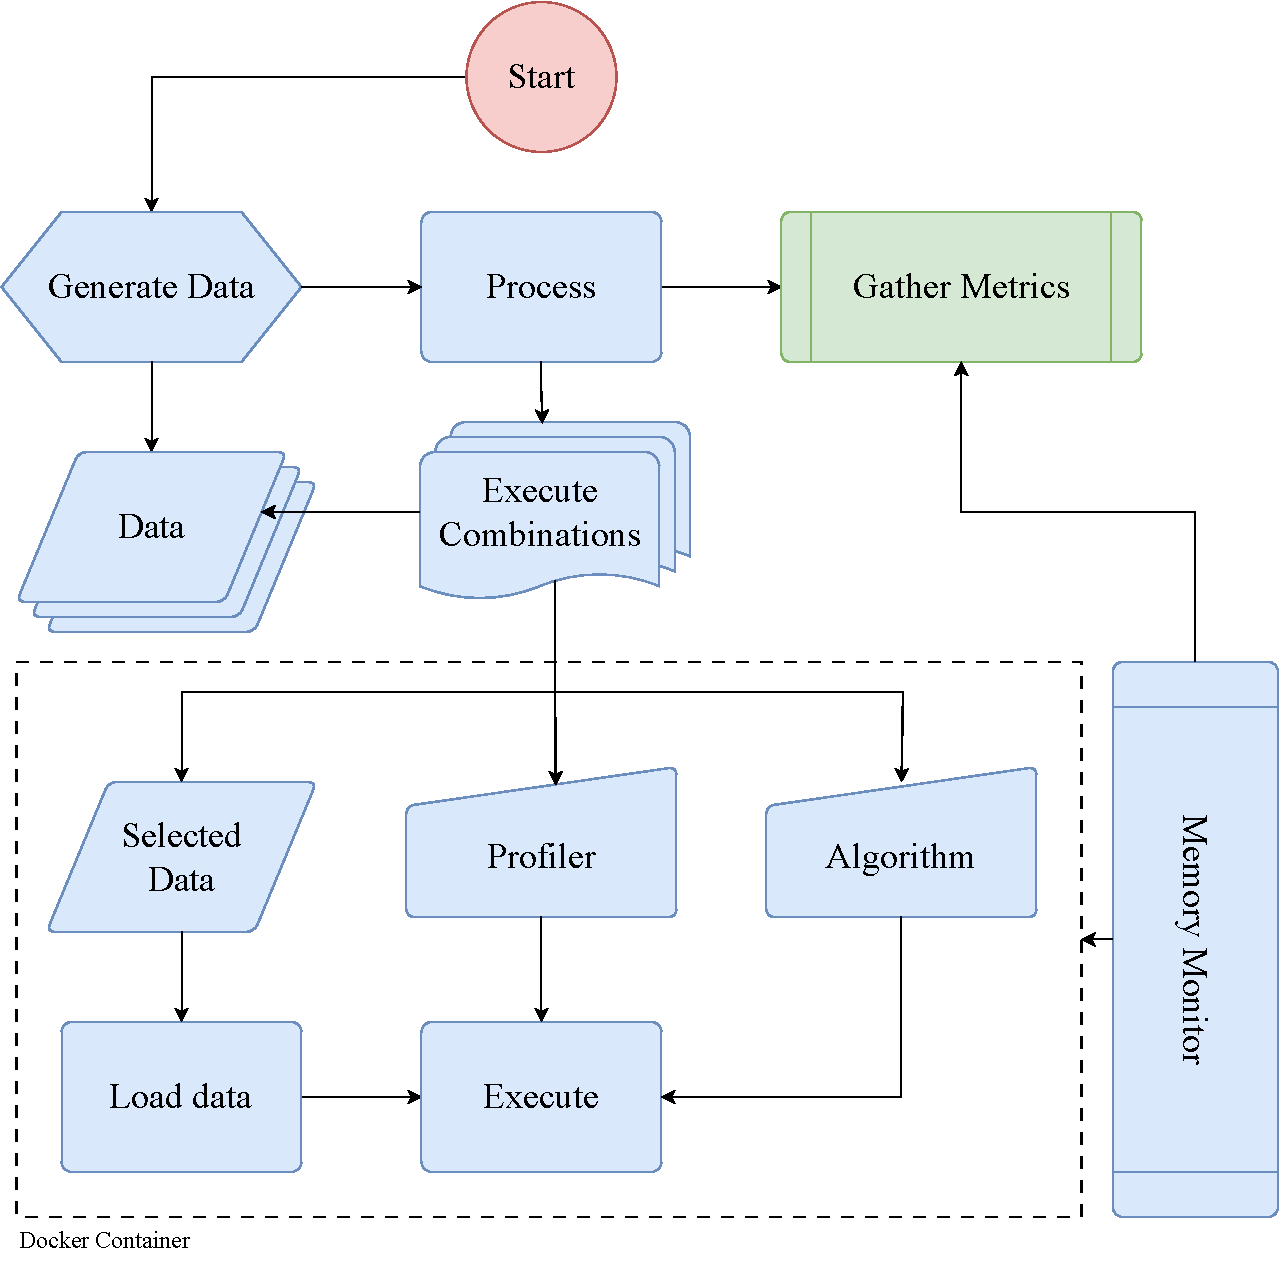
\includegraphics[width=0.8\textwidth]{./assets/images/04-experiment-flowchart}
%    \caption{Flowchart illustrating the memory consumption experiment workflow.}
%    \label{fig:mmc-experiment-workflow}
%\end{figure}
%
%\subsection{Evaluation Methodology}
%\label{subsec:mmc-evaluation-methodology}
%
%The evaluation of the experimental results was conducted using a multi-faceted approach that integrates statistical analysis and validation techniques.
%This comprehensive methodology ensures that the analysis is both rigorous and reliable, providing meaningful insights into memory usage patterns, performance trends, and the computational efficiency of the algorithms.
%
%The primary focus of the evaluation was to analyze three key aspects: memory efficiency, performance trends over time, and execution performance.
%Each of these aspects offers a unique perspective on the algorithms’ behavior when analyzed with different profiling tools, enabling a comprehensive evaluation of the strengths and limitations of various memory measurement techniques.
%
%In addition to the primary analysis, two validation techniques were employed to verify the accuracy and reliability of the collected data.
%These validation methods ensure that the metrics accurately reflect the actual resource usage and performance characteristics of the experiments.
%
%Table~\ref{tab:mmc-evaluation-criteria} summarizes the evaluation criteria and validation techniques used in this study.
%
%\begin{table}[h]
%    \centering
%    \begin{tabular}{|l|p{6cm}|}
%        \hline
%        \textbf{Evaluation Criteria}     & \textbf{Description}                                                                                                                                                                                                                                 \\ \hline
%        Memory Efficiency                & Evaluates \Mpeak across different algorithms, datasets, and profiling tools. By comparing these values, we can identify the differences between each memory measurement technique.                                                                   \\ \hline
%        Performance Trends               & Analyzes \Mt to detect temporal consumption patterns, such as sudden spikes, gradual increases (indicative of memory leaks), and periods of stable usage.                                                                                            \\ \hline
%        Execution Performance            & Correlates memory consumption metrics with \T to assess the trade-offs between memory usage and processing speed, providing insights into computational efficiency.                                                                                  \\ \hline
%        Cross-Validation with Docker API & Verifies the internal memory usage data by comparing it with external monitoring results obtained through the Docker \ac{API}. This comparison helps ensure the consistency and reliability of the internal memory measurements.                     \\ \hline
%        Memory Constraint Validation     & Re-executes experiments under constrained memory conditions, with limits set slightly below the previously recorded \Mpeak. This validation confirms whether the measured \Mpeak represents the minimum memory requirement for successful execution. \\ \hline
%    \end{tabular}
%    \caption{Evaluation criteria and validation techniques for the memory consumption experiments}
%    \label{tab:mmc-evaluation-criteria}
%\end{table}
%
%The cross-validation with Docker \ac{API} data provided an external benchmark to verify the accuracy of the internal memory measurements.
%By comparing the internal data with Docker's resource metrics, we ensured that the recorded memory usage reflected the actual resource consumption of the containerized environments.
%
%Furthermore, the memory constraint validation served as a practical test to confirm the robustness of the peak memory usage measurements.
%By limiting the available memory to slightly below the recorded \Mpeak, we observed whether the algorithm could still execute successfully.
%Failure to complete the execution under these constrained conditions validated that the original \Mpeak measurement accurately represented the minimum memory required for the algorithm to run without errors.
%
%This comprehensive evaluation framework ensures that the analysis of memory consumption and performance is both thorough and reliable, providing meaningful insights into the behavior of the algorithms under various resource constraints.
%
%\subsection{Experiment Repository}
%\label{subsec:mmc-experiment-repository}
%
%You can find all the code, results, and experimental data used in the following repository: \DFTODO{Adicionar o link pro repositório}.
%
%
%\section{Experimental Results}
%\label{sec:mmc-results}
%
%\DFTODO{Demonstrar resultados dos experimentos com viés (sem controlar o ambiente). Mostrando o impacto de execuções anteriores}
%\DFTODO{Apresentar os resultados dos experimentos, mostrando o consumo de memória e o tempo de execução para cada algoritmo.}
%\DFTODO{Destacar a validação feita para garantir a precisão das medições. Encontrando a questão da pressão de memória}
%\DFTODO{Demonstrar o impacto ao aplicar pressão de memória}
%
%
%\section{Conclusion}
%\label{sec:mmc-conclusion}
%
%\DFTODO{Concluir a respeito da necessidade de ambientes controlados para medir a memória}
%\DFTODO{Concluir sobre as diferentes formas de medir a memória}
%\DFTODO{Concluir sobre o garbage collector e a possibilidade de executar com pressão de memória}
    \chapter{Predicting Memory Consumption from Input Shapes}
\label{ch:predicting-memory-consumption-from-input-shapes}

\section{Introduction}
\label{sec:pmc-introduction}

\ac{HPC} environments require users to specify computing resources, especially memory, before a job begins execution.
Common \ac{HPC} job schedulers, such as Slurm~\cite{yoo2003slurm} or \ac{PBS}~\cite{henderson1995pbs}, enforce fixed memory reservations at submission time.
This enforcement compels users to estimate a job's memory footprint in advance.
That requirement creates a fundamental challenge: users must predict memory needs \emph{a priori}, often without the benefit of trial runs.
Setting the memory request too low causes out-of-memory errors~\cite{bailey2005,hovestadt2003}, leading to lost computing time and queued tasks.
Setting it too high wastes memory and reduces overall system utilization because nodes retain unused allocations.
Accurate memory estimation therefore remains crucial for reliability and efficiency in \ac{HPC} resource management.

Most users rely on guesswork to determine memory reservations.
Many \ac{HPC} users adopt trial-and-error methods~\cite{ncsu_memory_usage}\EB{Tente substituir por uma referência a um artigo publicado.}, iteratively adjusting memory limits across repeated job submissions until one run completes without errors.
This approach leads to inefficiency and significant risk.
Each failed attempt wastes wall-clock time and computational cycles, while each successful run with excessive memory allocations deprives other jobs of available resources.
Over-provisioning represents a common workaround but leaves systems underutilized.
That trial-and-error paradigm reduces overall throughput and burdens users with resource-tuning responsibilities instead of scientific exploration.

Predictive modeling for memory allocation offers a clear path to improvement.
Models can forecast a job's memory demand using readily available workload features such as input data size, dimensionality, algorithmic parameters, or usage patterns from similar jobs.
These forecasts reduce guesswork and limit the need for iterative resubmissions.
More accurate pre-runtime memory predictions enable users to request memory more precisely, mitigating failure risks and alleviating resource waste~\cite{tanash2021ampro}.

The content in this chapter prioritizes \EBC{tensor-based}{tensor-based é usado aqui, mas array-based em usado mais à frente. Seria bom padronizar o uso destes termos. Além disso, tensor-based, tensor-centric e outros termos baseados em tensores aparecem aqui mas não foram definidos. Seria bom definí-los no primeiro uso do termo.} workloads, which exhibit strong correlations between memory usage and input shape.
Numerous scientific and data-centric applications center on large multidimensional arrays, known as tensors.
Examples include seismic wave simulations on \ac{3D} grids, high-resolution image analysis in computer vision, and large-scale numerical linear algebra routines in scientific computing.
Memory consumption in these scenarios often scales according to array dimensions, because storage for input data structures and intermediate results typically dominates memory usage.
For example, doubling the resolution of an input image in each dimension roughly quadruples its memory footprint~\cite{stackoverflow_memory_inv}, while in deep neural networks increasing either input size or batch size similarly amplifies memory usage due to larger activation maps and additional computation~\cite{dell_3dunet_memory}.
These relationships underscore the crucial role of input shape in determining memory demands for tensor-centric workloads.
A predictive model that captures how memory scales with shape parameters can then offer robust estimates for new input configurations.

Several research directions have explored memory usage estimation and prediction in related fields.
In the \ac{HPC} domain, historical job data from systems like Slurm often enable machine learning models to predict resource consumption.
These models exploit features such as job metadata and input sizes to forecast memory requirements~\cite{yoo2003slurm}.
That approach demonstrates that ample historical data can support reliable predictions for recurring workloads.
In high-level numerical computing, analytical modeling of memory for array operations provides another possibility~\cite{cornell_memory_workshop}.
Matrix multiplications, convolutions, and other array-based methods can be studied to deduce peak memory usage without full execution.
Deep learning frameworks take a similar route to anticipate a network's memory footprint.
Layer-by-layer analysis of network architectures and input tensor dimensions reveals how memory usage accumulates~\cite{gao2020, dell_3dunet_memory}.
Profiling and simulation tools further assist deployment decisions by projecting memory usage before runtime~\cite{tanash2019}.

The primary objective of the present chapter is to estimate memory usage for new jobs given their input shapes, rather than to yield an exact byte-level measurement.
This emphasis on practical accuracy aims to provide a sufficiently precise estimate of peak memory demand to guide resource allocation.
Slight discrepancies arise due to overheads and system factors, but a well-calibrated predictor avoids severe underestimates that result in \ac{OOM} failures.
Focusing on a reliable upper-bound estimate allows users to reserve memory with greater confidence.
Narrowing the gap between requested and consumed memory improves performance over purely heuristic-based approaches and alleviates the risks and inefficiencies commonly associated with guesswork.
\section{Materials and Methods}
\label{sec:pmc-materials-and-methods}

This section explains the complete methodology for gathering memory-consumption data, generating shape-based features, and training predictive models.
The overall pipeline includes four core phases.
(i) Data Generation,
(ii) Memory Profiling,
(iii) Result Collection,
and (iv) Analysis.
These phases ensure consistent, reproducible, and high-quality measurements, which support machine learning models that learn memory usage from shape attributes.

\vspace{1em}
\noindent
\textbf{Phase 1: Data Generation.}
The experiment begins with synthetic seismic datasets.
In a typical seismic application, three dimensions describe the data.
\emph{inlines}, \emph{xlines}, and \emph{samples}.
The script systematically enumerates shape configurations by varying these dimensions from an \texttt{INITIAL\_SIZE} to a \texttt{FINAL\_SIZE} with increments of \texttt{STEP\_SIZE}.
For example, when the initial size equals 100, the final size equals 600, and the step size equals 100, the script generates volumes of sizes
\(\{\,(100,100,100),\,(100,100,200),\dots,(600,600,600)\}\)
and writes them to \ac{SEG-Y}~\cite{barry1975segy} files.
These synthetic datasets mimic actual seismic data and span diverse volumes to reveal how memory grows with increasing dimension sizes.

\vspace{1em}
\noindent
\textbf{Phase 2: Memory Profiling.}
A shell script schedules container-based jobs to run seismic operators on each generated dataset.
Chapter~\ref{ch:measuring-memory-consumption} describes the \ac{HPC}-like constraints and the rationale for isolating each job to reduce interference.
Accordingly, the script starts \ac{dind} containers pinned to specific \ac{CPU} cores through \texttt{--cpuset-cpus}.
This binding ensures comparable runs.
The script then processes three main operators:

\begin{itemize}
    \item \emph{Envelope}~\cite{taner1979complex}: A classic seismic attribute that computes instantaneous amplitude for each trace.
    \item \emph{\ac{GST3D}}~\cite{bigun2004recognition}: A structural attribute designed to highlight seismic faults or discontinuities.
    \item \emph{3D Gaussian Filter}~\cite{gonzalez2002digital}: A spatial smoothing operator for seismic volumes.
\end{itemize}

Each operator appears as a Docker image defined in the \texttt{Dockerfile}.
Each container execution uses a Python script to load and process input data.
The \texttt{traceq} library records \ac{RSS} over time, as \EBRP{shown}{discussed} in Chapter~\ref{ch:measuring-memory-consumption}.
On completion, a \texttt{.prof} file stores the memory timeline and associated metadata, including timestamps and shape parameters.
This procedure captures peak memory usage accurately.

\vspace{1em}
\noindent
\textbf{Executing Operators and Gathering Profiles.}
Listing~\ref{lst:exp_sh} shows portions of the shell script.
The script orchestrates the sequence.
(i) create Docker volumes,
(ii) run a Python script to generate the synthetic datasets,
(iii) for every generated \ac{SEG-Y} file, execute Envelope, \ac{GST3D}, or Gaussian Filter,
(iv) run a Python script to parse and consolidate measurements,
and (v) finalize executing another Python script for exploratory data analysis.
Each run deposits output \ac{CSV} files and profiles in designated \texttt{OUTPUT\_DIR} subdirectories.

\vspace{1em}
\begin{lstlisting}[style=bashstyle,caption={Excerpts from \texttt{experiment.sh}~\cite{delucca2025experiment2script} that orchestrate Docker-based runs. Variables like \texttt{DATASET\_FINAL\_SIZE} and \texttt{DATASET\_STEP\_SIZE} define shape ranges for dataset generation.}, label={lst:exp_sh}]
#!/usr/bin/env sh
TIMESTAMP="$(date +%Y%m%d%H%M%S)"
CPUSET_CPUS="0"
DATASET_FINAL_SIZE="800"
DATASET_STEP_SIZE="50"

echo "Generating input data..."
docker run \
  --cpuset-cpus=0 \
  -v "${DIND_VOLUME_NAME}:/var/lib/docker:rw" \
  ...
  --env EXPERIMENT_COMMAND="generate_data.py" \
  --env EXPERIMENT_ENV="\
    -e OUTPUT_DIR=/experiment/out \
    -e FINAL_SIZE=${DATASET_FINAL_SIZE} \
    -e STEP_SIZE=${DATASET_STEP_SIZE} \
  " \
  docker:28.0.1-dind \
  "/workspace/experiment.sh"

echo "Collecting memory profile for Envelope..."
for file in "${OUTPUT_DIR}/inputs"/*.segy; do
  filename=$(basename "$file" .segy)
  docker run \
    --cpuset-cpus=0 \
    ...
    --env EXPERIMENT_COMMAND="collect_memory_profile.py" \
    --env EXPERIMENT_ENV="\
      -e ALGORITHM=envelope \
      -e INPUT_PATH=/experiment/out/inputs/${filename}.segy \
    " \
    docker:28.0.1-dind \
    "/workspace/experiment.sh"
done
...
\end{lstlisting}

\noindent
Table~\ref{tab:env_vars} summarizes relevant environment variables used by these scripts.
They control dataset sizes, repetition counts, and output paths.

\begin{table}[htbp]
    \centering
    \caption{Key environment variables for the experimental scripts.
    Defaults appear in parentheses.
    \vspace{1em}}
    \label{tab:env_vars}
    \begin{tabular}{ll}
        \hline
        \textbf{Variable}             & \textbf{Description}                                                                        \\
        \hline
        \texttt{DATASET\_FINAL\_SIZE} & Final dimension size (e.g., 800)                                                            \\
        \texttt{DATASET\_STEP\_SIZE}  & Step size between dimension increments (e.g., 50)                                           \\
        \texttt{EXPERIMENT\_N\_RUNS}  & Number of repeated runs per shape (e.g., 30)                                                \\
        \texttt{CPUSET\_CPUS}         & \ac{CPU} core pinning for Docker containers (e.g., 0)                                       \\
        \texttt{OUTPUT\_DIR}          & Directory for output profiles, logs, and \texttt{\ac{CSV}} files                            \\
        \texttt{ALGORITHM}            & Selected operator (e.g., \texttt{envelope}, \texttt{\ac{GST3D}}, \texttt{gaussian\_filter}) \\
        \hline
    \end{tabular}
\end{table}

\vspace{1em}
\noindent
\textbf{Phase 3: Results Collection and Feature Construction.}
This phase consists in evaluating the \texttt{.prof} files output by \texttt{traceq}, extracting peak memory usage, and associating it with the input shape.
The script identifies \EBC{inlines, xlines, and samples}{estes três termos aparecem com formatação distintas ao longo do texto - normal, itálico e negrito. Não ficou claro para mim por que eles são destacados de forma distinta. Seria bom padronizar a forma de formatar estes termos.} from filenames, notes the operator, retains the maximum time-series \ac{RSS} value, and compiles a consolidated dataframe.
It also derives extended features such as total volume
(\(\text{inlines} \times \text{xlines} \times \text{samples}\)),
logarithmic transforms
(e.g., \(\log_2(\text{volume})\)),
surface area,
dimension ratios,
and polynomial expansions.
These features capture various ways shape correlates with peak memory usage.
Listing~\ref{lst:results_py} shows how this phase generates and transforms these features.

\begin{lstlisting}[style=pythonstyle,
    caption={Feature extraction excerpt from \texttt{collect\_results.py}~\cite{delucca2025experiment2resultscollection}. Additional derived metrics capture polynomial or ratio-based growth.},
    label={lst:results_py}]
df_features["volume"] = (
    df_features["inlines"]
    * df_features["xlines"]
    * df_features["samples"]
)

df_features["diagonal_length"] = np.sqrt(
    df_features["inlines"]**2
    + df_features["xlines"]**2
    + df_features["samples"]**2
)

df_features["surface_area"] = 2 * (
    df_features["inlines"] * df_features["xlines"]
    + df_features["inlines"] * df_features["samples"]
    + df_features["xlines"] * df_features["samples"]
)

df_features["log_inlines"] = np.log2(df_features["inlines"])
df_features["log_volume"] = np.log2(df_features["volume"])
...
\end{lstlisting}

\vspace{1em}
\noindent
\textbf{Phase 4: Model Training and Analysis.}
The script from phase 3 trains multiple regression models using \texttt{inlines}, \texttt{xlines}, \texttt{samples}, and derived features as predictors.
Peak memory usage acts as the target variable.
A consistent 80/20 training/test split ensures fair comparisons.
Envelope, \ac{GST3D}, and Gaussian Filter runs each receive separate analyses.
Performance metrics include \ac{RMSE}~\cite{hyndman2006}, \ac{MAE}~\cite{willmott2005mae}, $R^2$~\cite{draper1998applied}, and an \EBC{accuracy score that measures the fraction of predictions within a specified relative error}{Tem que descrever como este score é calculado}.
An \texttt{Optuna}-based~\cite{akiba2019optuna} parameter search can emphasize safe upper-bound estimates in \ac{HPC} contexts where underestimations produce critical failures.
The following models form the basis of each comparison:

\begin{itemize}
    \item \textbf{Linear Regression, Polynomial Regression}~\cite{hastie2009elements}\\
    These models create foundational baselines to capture the relationship between features and memory usage.
    Linear regression indicates whether memory usage scales directly with \EBC{trace or sample counts}{não seria mais preciso dizer "any of the features, suach as trace or smaple counts"?}.
    Polynomial regression extends linear models with higher-order terms to account for mild nonlinearities.
    Caution is required since purely linear fits underfit complex relationships, and high-degree polynomials risk overfitting.

    \item \textbf{Decision Trees}~\cite{breiman1984classification}, \textbf{Random Forest}~\cite{breiman2001random}, \textbf{\ac{XGBoost}}~\cite{chen2016xgboost}\\
    \EB{Lembre-se de revisar a versão final para identificar e corrigir eventuais invasões de margem, como acima.}
    These tree-based methods automatically model complex feature interactions and nonlinearities.
    Decision Trees provide easy interpretability and can indicate shape thresholds that strongly affect memory.
    Random Forest aggregates multiple trees to reduce variance and enhance generalization.
    \ac{XGBoost} incrementally refines an ensemble of weak learners, which often results in higher accuracy on structured data.
    Hyperparameter tuning (e.g., tree depth or learning rate) is essential to avoid overfitting. \EB{Seria bom adicionar uma referência para dar suporte a este comentário.}

    \item \textbf{Neural Networks (\ac{MLP})}~\cite{rumelhart1986learning}\\
    \ac{MLP} architectures can approximate intricate functions when provided sufficient capacity.
    This property can reveal subtle relationships between shape parameters and memory requirements.
    These models often demand larger datasets, rigorous hyperparameter optimization, and careful overfitting control. \EB{Seria bom adicionar uma referência para dar suporte a este comentário.}

    \item \textbf{Gaussian Processes}~\cite{rasmussen2006gaussian}\\
    This approach offers both mean predictions and uncertainty estimates.
    Uncertainty bounds are especially valuable in \ac{HPC} scenarios where underestimating memory can cause abrupt job failures.
    Large datasets pose computational challenges because of the \(O(n^3)\) scaling, and kernels must be selected carefully. \EB{Seria bom adicionar uma referência para dar suporte a este comentário.}

    \item \textbf{Bayesian Ridge Regression}~\cite{bishop2006pattern}\\
    This extension of linear models applies Bayesian inference to estimate coefficients and yields robust predictions with uncertainty quantification.
    HPC workloads benefit from these uncertainty estimates when resource over-provisioning is less harmful than running out of memory.
    Polynomial or interaction terms might still be necessary to represent nonlinear growth patterns. 
\end{itemize}

The script final Python script then visualizes memory distributions, residual plots, feature evaluations, and data-reduction experiments.
This exploration reveals each model’s generalization capacity, indicates which features add minimal value, and evaluates the number of training examples that the predictive framework requires.
Partial dependence plots and tree-based model interpretations expose how inlines, xlines, and samples exert the highest influence on memory usage.

\vspace{1em}
\noindent
\textbf{Technical Considerations.}
\begin{itemize}
    \item \emph{Containerization and Reproducibility:}
    Each stage runs in a Docker container with pinned versions of Python packages.
    This standardized environment preserves consistent results by preventing version drift.
    \item \emph{\ac{CPU} Affinity:}
    The \texttt{--cpuset-cpus=0} parameter restricts execution to a single core and reduces background noise.
    Multiple runs per dataset shape (\texttt{EXPERIMENT\_N\_RUNS}) further \EBC{stabilize measurements.}{accounts for stochatic variance?}
    \item \emph{Parallelization:}
    The Docker orchestration scales to multiple \ac{CPU} cores, but the design imposes single-core experiments for repeatability.
    Actual \ac{HPC} clusters manage concurrency at the scheduler level, but the core principle of shape-driven memory profiling remains applicable.
    \item \emph{Cache Handling:}
    Chapter~\ref{ch:measuring-memory-consumption} recommends dropping Linux memory caches to eliminate carry-over effects.
    This option appears in the scripts to ensure a clean environment for memory measurements.
\end{itemize}

\vspace{1em}
\noindent
Figure~\ref{fig:pmc_datapipeline} illustrates the entire workflow.
The process generates synthetic \ac{SEG-Y} volumes, runs containerized operators for memory profiling, and consolidates results into a final dataset that links shape features to peak memory usage.
Regression models then learn to map input dimensions to memory demand.
Section~\ref{sec:pmc-results} elaborates on these experimental outcomes and compares the predictive accuracy of the considered models.

\begin{figure}[htbp]
    \centering
    \resizebox{\textwidth}{!}{
        \begin{tikzpicture}[
            font=\sffamily\small,
            phase/.style={
                draw=black,
                thick,
                fill=gray!10,
                rectangle,
                rounded corners,
                drop shadow,
                align=center,
                minimum width=3.8cm,
                inner sep=0.4cm
            },
            box/.style={
                draw=black,
                thick,
                fill=white,
                rectangle,
                rounded corners,
                align=center,
                minimum width=3.8cm,
                minimum height=1.1cm
            },
            arrow/.style={
                ->,
                thick
            },
            node distance=0.4cm and 0.8cm
        ]

            % Phase 1: Data Generation
            \node[phase] (phase1) {Phase 1:\\Data Generation};
            \node[box, below=of phase1] (p1input) {\textbf{Input}\\Shape parameters\\(inlines, xlines, samples)};
            \node[box, below=of p1input] (p1process) {\textbf{Process}\\Generate synthetic\\SEG-Y volumes};
            \node[box, below=of p1process] (p1output) {\textbf{Output}\\Synthetic data files};

            \draw[arrow] (p1input) -- (p1process);
            \draw[arrow] (p1process) -- (p1output);

            % Phase 2: Memory Profiling
            \node[phase, right=3cm of phase1] (phase2) {Phase 2:\\Memory Profiling};
            \node[box, below=of phase2] (p2input) {\textbf{Input}\\Synthetic SEG-Y files};
            \node[box, below=of p2input] (p2process) {\textbf{Process}\\Container-based\\operators (traceq)};
            \node[box, below=of p2process] (p2output) {\textbf{Output}\\.prof files};

            \draw[arrow] (p2input) -- (p2process);
            \draw[arrow] (p2process) -- (p2output);
            \draw[arrow] (p1output.east) -- ++(0.7,0) |- (p2input.west);

            % Phase 3: Feature Aggregation
            \node[phase, right=3cm of phase2] (phase3) {Phase 3:\\Aggregation \& Feature\\Construction};
            \node[box, below=of phase3] (p3input) {\textbf{Input}\\.prof files + shape info};
            \node[box, below=of p3input] (p3process) {\textbf{Process}\\Parse peak usage\\Derive features};
            \node[box, below=of p3process] (p3output) {\textbf{Output}\\Feature dataset};

            \draw[arrow] (p3input) -- (p3process);
            \draw[arrow] (p3process) -- (p3output);
            \draw[arrow] (p2output.east) -- ++(0.7,0) |- (p3input.west);

            % Phase 4: Model Training
            \node[phase, right=3cm of phase3] (phase4) {Phase 4:\\Model Training \& Evaluation};
            \node[box, below=of phase4] (p4input) {\textbf{Input}\\Feature dataset};
            \node[box, below=of p4input] (p4process) {\textbf{Process}\\Train regression\\(XGBoost, NN, etc)};
            \node[box, below=of p4process] (p4output) {\textbf{Output}\\Memory usage\\predictions};

            \draw[arrow] (p4input) -- (p4process);
            \draw[arrow] (p4process) -- (p4output);
            \draw[arrow] (p3output.east) -- ++(0.7,0) |- (p4input.west);

        \end{tikzpicture}
    }
    \caption{Schematic of the memory prediction pipeline. It includes synthetic data generation, containerized profiling, feature extraction, and regression model training.}
    \label{fig:pmc_datapipeline}
\end{figure}
\section{Experimental Setup}
\label{sec:pmc-experimental-setup}

The experiment followed a pipeline composed of seismic data generation, containerized processing with memory profiling, and consolidation of results for modeling.
Each step was fully automated to ensure consistency, reproducibility, and scalability.
The subsections below detail the execution environment, data generation, operator processing, memory profiling, and data consolidation strategies.

\subsection{Execution Environment and Workflow Automation}
\label{subsec:pmc-execution-environment-and-workflow-automation}

All experiments \EBADD{were} executed on a single \ac{HPC} node at the \ac{UNICAMP} Discovery Labs, equipped with an Intel\textregistered\ Xeon\textregistered\ Silver 4310 processor, 256~\ac{GB} of \ac{RAM}, and two \ac{RTX}~A6000 \ac{GPU}s. Despite the presence of \ac{GPU} resources, all memory profiling runs relied exclusively on \ac{CPU} execution to ensure comparability across input shapes.

A Python-based container environment managed via Docker provided reproducibility and isolation.
Docker containers pinned to specific \ac{CPU} cores (\texttt{–cpuset-cpus=0}) maintained execution consistency and minimized process interference.

A single shell script, \texttt{scripts/experiment.sh}\cite{delucca2025experiment2script}, orchestrated the full workflow, including:
\begin{enumerate}
    \item Creation of Docker volumes for intermediate and output data storage.
    \item Generation of synthetic \ac{3D} seismic volumes, as described in Section\ref{sec:pmc-materials-and-methods}.
    \item Execution of seismic operators within containers, \EBC{one run per input shape configuration}{Não deveriam ser múltiplas execuções? Qual o valor da variável \texttt{EXPERIMENT\_N\_RUNS}?}.
    \item Memory profiling using \texttt{TraceQ}, which captured \ac{RSS} measurements over time.
    \item Extraction and consolidation of peak memory values, shape metadata, and execution logs into structured \texttt{.csv} files.
\end{enumerate}

The script looped over all permutations of \texttt{(inlines, xlines, samples)}, parsing \texttt{TraceQ} outputs and joining them with shape metadata.
The final output consisted of a consolidated dataset for model fitting.

\subsection{Synthetic Data Generation and Real-Data Validation}
\label{subsec:pmc-synthetic-data-generation-and-real-data-validation}

\paragraph{Synthetic Volumes.}
A comprehensive enumeration of \ac{3D} input shapes defined the experimental space.
Input volumes ranged from $100$ $\times$ $100$ $\times$ $100$ to shapes approaching system memory limits.
Each synthetic volume was written in the \ac{SEG-Y} format to maintain consistency with the seismic processing pipeline.
This method enabled a controlled exploration of both common and extreme input configurations.

\paragraph{Netherlands F3 Dataset~\cite{f3dataset}.}
The standard Netherlands F3 seismic volume ($651$ $\times$ $951$ $\times$ $462$) served as a real-data validation benchmark.
Memory usage predictions from the trained models were compared against actual measurements on this dataset, enabling evaluation of model generalization to real-world data.

\subsection{Containerized Seismic Operators and Memory Profiling}
\label{subsec:containerized-seismic-operators-and-memory-profiling}

Each shape configuration was processed in a dedicated Docker container with exclusive \ac{CPU} pinning to reduce runtime variance.
Three memory-intensive seismic operators were evaluated: \emph{Envelope}, \emph{\ac{GST3D}}, and a \emph{3D Gaussian Filter}.
These operators were treated as black-box transformations that received seismic volumes and returned transformed data, with no internal modifications or visibility into their implementation.

The container startup routine activated \texttt{TraceQ}, which monitored the Python process and recorded \ac{RSS} snapshots at regular intervals.
Upon operator completion, \texttt{TraceQ} wrote a \texttt{.prof} file containing the memory usage timeline.
This design minimized noise from external processes and ensured that each memory profile reflected the specific behavior of the evaluated operator and input shape.

\subsection{Data Consolidation}
\label{subsec:data-consolidation}

After execution, a final stage of the script merged experimental data into a unified dataset.
The consolidation included:

\begin{itemize}
    \item \textbf{Peak Memory Values:} Extracted from each \texttt{.prof} file as the highest recorded \ac{RSS}.
    \item \textbf{Shape and Operator Metadata:} Inline, xline, and sample dimensions, as well as the applied seismic operator and associated attributes.
    \item \textbf{Derived Features:} Calculated values such as total volume (\text{inlines} $\times$ \text{xlines} $\times$ \text{samples}), logarithmic transformations, and geometric descriptors including surface area and diagonal length.
\end{itemize}

This merged dataset was stored in structured \EBC{\texttt{.csv} files}{em outros locais do texto você usa o termo CSV file - seria bom padronizar. BTW, o acrônimo CSV deve ser definido na lista de acrônimos.} under \texttt{OUTPUT\_DIR}, forming the foundation for subsequent modeling and analysis.

\subsection{Repository Structure and Notebooks}
\label{subsec:repository-structure-and-notebooks}

\EB{Daniel, acho que é bem importante ter uma seção com instruções para reprodução dos experimentos. Ela deve descrever de onde o leitor pode baixar os códigos e dados e como executar os artefatos. Acho que esta seção poderia ser ajustada para cumprir este papel. Neste sentido, que tal renomeá-la para "Reproducibility" e adicionar instruções de como baixar e executar os artefatos?}

\EB{BTW, recentemente a Unicamp introduziu um requisito novo para a defesa do mestrado e do doutorado que consiste no depósito dos artefatos produzidos durante a pesquisa no repositório de dados da Unicamp - REDU.  Veja em \url{https://ic.unicamp.br/pos-graduacao/repositorio-de-dados-de-pesquisa-da-unicamp-redu/}}

The entire experiment, including code, automation scripts, and analytical notebooks, is publicly available:
\begin{itemize}
    \item \textbf{\texttt{Github repository}}\cite{delucca2025experiment2} containing all source code and setup instructions.
    \EB{Por favor, migre estes repositórios para a (ou crie uma cópia deles na) organização \url{https://github.com/discovery-unicamp} e refenrencie o endereço de lá.}
    \item \textbf{\texttt{scripts/experiment.sh}}\cite{delucca2025experiment2script} for end-to-end execution of data generation, processing, and profiling.
    \item \textbf{\texttt{notebooks/}}~\cite{delucca2025experiment2notebooks} with Jupyter notebooks covering data exploration, model training, hyperparameter optimization, and error diagnostics.
\end{itemize}

This structure ensures full reproducibility.
Users can extend the experiment by modifying input shapes, seismic operators, or container settings without altering the orchestration logic.
All components—containers, execution scripts, and analytical workflows—remain tightly integrated to support extensibility and transparent evaluation.
\section{Experimental Results}
\label{sec:pmc-results}

This section presents comprehensive results for predicting memory consumption in seismic workloads based on their \ac{3D} input shapes.
We organize the findings into four main categories:
(i) memory and execution-time profiling,
(ii) model performance overview,
(iii) feature selection experiments,
and (iv) data reduction studies.
Each category reveals different facets of how shape parameters affect resource requirements, model behavior, and prediction robustness.
All code, scripts, and output files that underlie these analyses reside in the \texttt{experiment} directory of the project repository~\cite{delucca2025experiment2results}.

\subsection{Experiment Outputs Overview}
\label{subsec:pmc-results-experiment-outputs-overview}

This subsection briefly outlines the three seismic operators examined (Envelope, \ac{GST3D}, and the 3D Gaussian Filter), underscores the main experimental objectives, and describes the key \ac{CSV} files generated during the final stages of the pipeline.
These \ac{CSV} artifacts are the foundation for the analyses presented in the following subsections.

\vspace{1em}
\noindent
\textbf{Operators and Experimental Goals.}
We investigated three commonly used seismic processing operators:
\begin{itemize}
    \item \emph{Envelope}: Computes instantaneous amplitude along seismic traces. 
    \item \emph{\ac{GST3D}}: Highlights discontinuities or faults using structural tensors.
    \item \emph{3D Gaussian Filter}: Applies a smoothing operation across volumes to reduce high-frequency noise.
\end{itemize}
All three involve memory-intensive operations on potentially large \ac{3D} volumes.
Our primary goal was to build regression models that predict each operator’s peak memory usage as a function of shape parameters (\textit{inlines}, \textit{xlines}, and \textit{samples}), enabling more accurate \ac{HPC} job submissions.

\vspace{1em}
\noindent
\textbf{Data Artifacts.}
During the final stage of the pipeline, five main \ac{CSV} outputs were generated:
\begin{enumerate}
    \item \emph{profile\_history.csv}: Stores time-series \ac{RSS} measurements and timestamps for each operator run. This file is useful for \EBRPD{detecting}{analyzing} moment-to-moment memory fluctuations.
    \item \emph{profile\_summary.csv}: Summarizes peak memory usage, execution time, and statistical descriptors (means, standard deviations, minima, and maxima) per volume configuration.
    \item \emph{model\_metrics.csv}: Captures regression model performances (\ac{RMSE}, \ac{MAE}, $R^2$, and accuracy metrics), along with arrays of predictions and residuals.
    \item \emph{feature\_selection.csv}: Documents experiments that limit the predictor set to specific features or transformations to assess their importance in predicting memory usage.
    \item \emph{data\_reduction.csv}: Compares how models behave when trained on progressively smaller subsets of the full dataset, providing insight into data requirements for stable predictions.
\end{enumerate}

\vspace{1em}
\noindent
\textbf{Shape Configurations.}
The synthetic seismic volumes encompassed a broad range of \ac{3D} shapes, from $100 \times 100 \times 100$ up to sizes near the system’s memory limits.
By spanning both small and large volumes, we could characterize memory usage trends across diverse problem scales.
Each operator was run on each shape variant, yielding a comprehensive grid of memory and runtime measurements.

\vspace{1em}
\noindent
\textbf{Chapter Roadmap.}
\EB{Acho que fica melhor remover o título "Chapter Roadmap." deste parágrafo.}
Section~\ref{sec:pmc-results-memory-and-execution-time-profiling} explores the memory-usage trends and execution-time patterns for each operator.
Subsequent sections delve into model performance, assessing how various feature sets and data volumes influence predictive accuracy.
We conclude by comparing Envelope, \ac{GST3D}, and Gaussian Filter side by side, identifying operator-specific nuances that can inform more reliable \ac{HPC} scheduling.
\section{Memory and Execution-Time Profiling}
\label{sec:pmc-results-memory-and-execution-time-profiling}

In this section, we focus on raw memory and execution-time measurements before discussing any modeling approach.
By examining usage patterns, run durations, and dimension-specific behaviors, we contextualize the challenges of predicting peak memory consumption in an \ac{HPC} setting.

\subsection{Linear Trends and Variability}
\label{subsec:linear-trends-and-variability}

Figure~\ref{fig:peak_memory_facet} shows how average peak memory usage tends to scale linearly with the overall volume (\(\text{inlines} \times \text{xlines} \times \text{samples}\)). 
\EB{Para refletir: Daniel, este gráfico por si só já mostra que existe uma relação quase linear entre a feature volume e o consumo de memória destes kernels. Fiquei na dúvida se faz sentido ter toda uma discussão sobre a relação entre as outras features e o consumo de memória depois de já concluir que há uma relação simples (linear) entre a feature volume e consumo de memória.}
The Envelope, \ac{GST3D}, and Gaussian Filter operators each display a relatively direct proportionality between volume and memory demand.
Interestingly, larger volumes produce consistently higher yet less variable memory consumption, whereas smaller volumes display higher \ac{CV}\EBRM{(coefficient of variation)}.

A possible explanation for this disparity is that smaller volumes involve shorter-run processes in which overheads (e.g., Python interpreter initialization, I/O buffering) can appear more prominently, thus creating variability.
As volumes grow, these overheads become negligible compared to the large data arrays and associated computations.
Consequently, memory usage “smooths out” and increasingly reflects the operator’s intrinsic workload characteristics.

\begin{figure*}[htbp]
    \centering
    \begin{subfigure}[t]{0.49\textwidth}
        \centering
        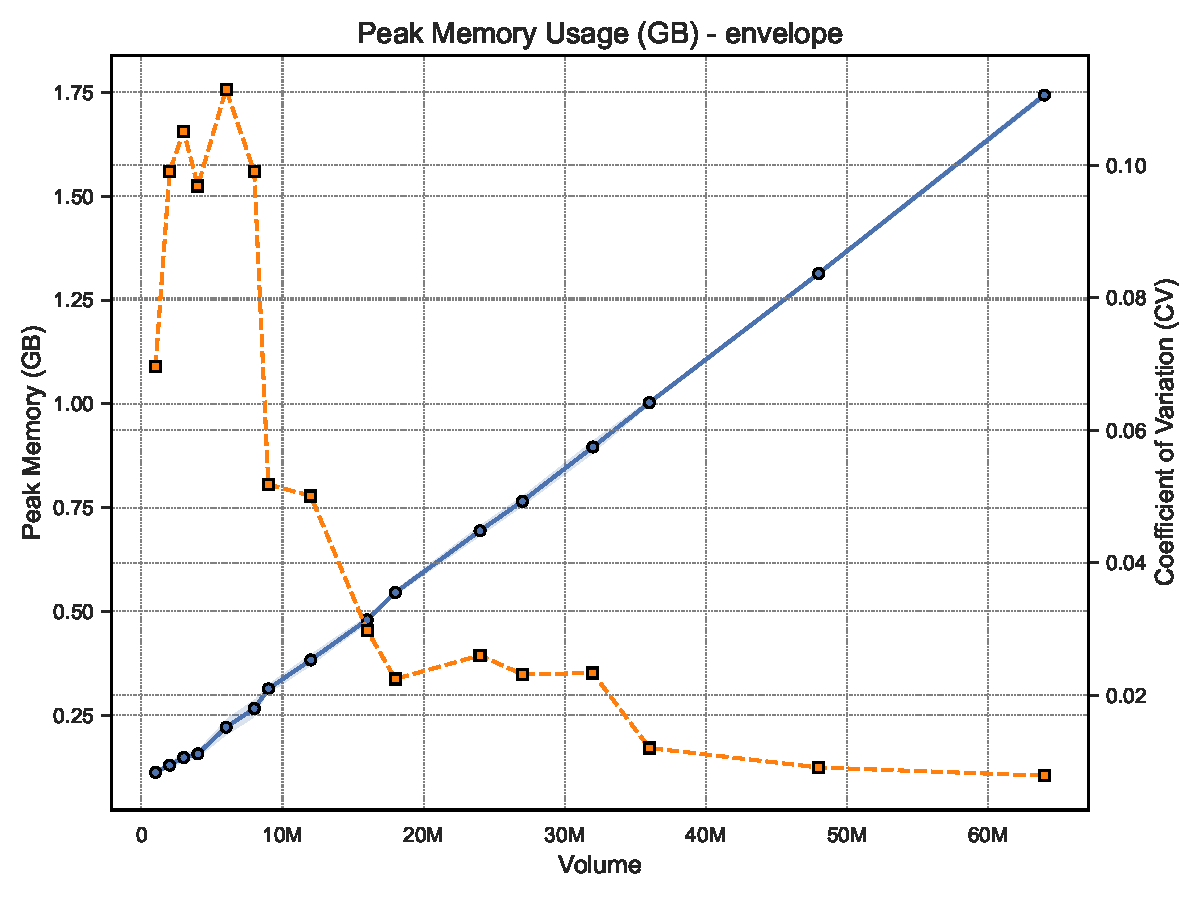
\includegraphics[width=\textwidth]{assets/images/05/peak_memory_by_volume_envelope}
        \caption{Envelope: Smaller volumes exhibit higher variability, while larger volumes show a consistent linear growth trend.}
    \end{subfigure}
    \hfill
    \begin{subfigure}[t]{0.49\textwidth}
        \centering
        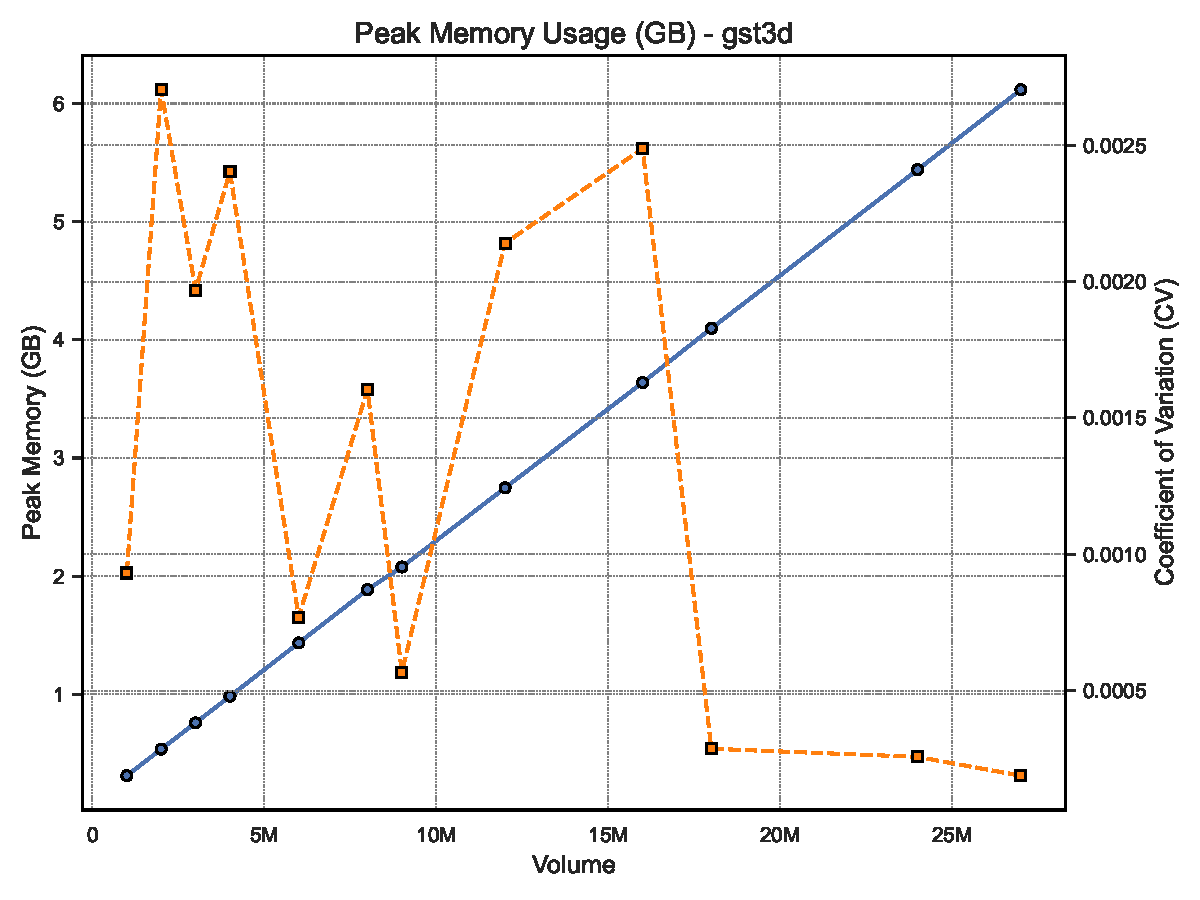
\includegraphics[width=\textwidth]{assets/images/05/peak_memory_by_volume_gst3d}
        \caption{\ac{GST3D}: This operator has a steeper slope compared to Envelope, reflecting more elaborate data structures.}
    \end{subfigure}
    \hfill
    \begin{subfigure}[t]{0.49\textwidth}
        \centering
        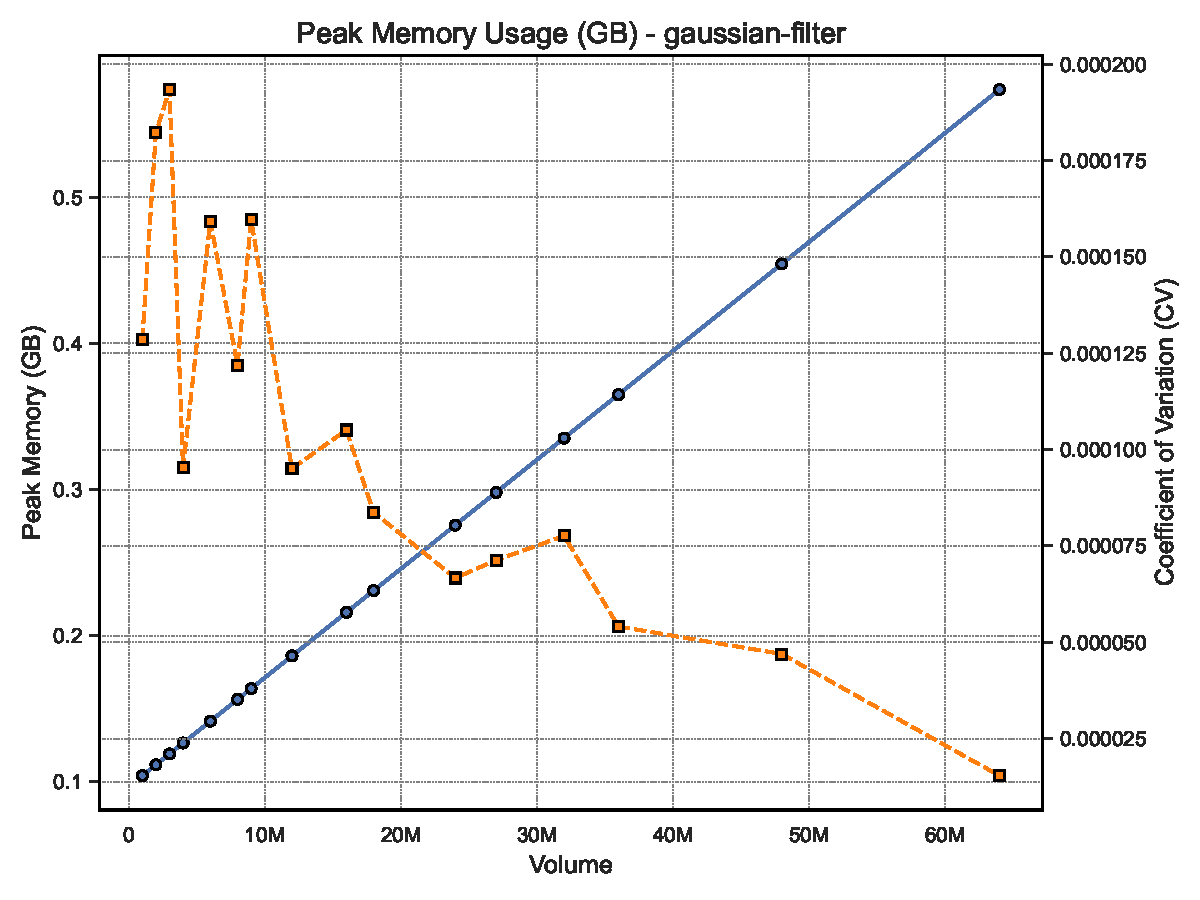
\includegraphics[width=\textwidth]{assets/images/05/peak_memory_by_volume_gaussian-filter}
        \caption{Gaussian Filter: Memory usage also scales linearly but with a gentler slope than \ac{GST3D}.}
    \end{subfigure}
    \caption{Peak memory usage by volume for Envelope, \ac{GST3D}, and Gaussian Filter. 
        Each operator shows an approximate linear growth rate as volume increases, but the slope and variability differ.
        \EB{Verifique se é possível usar o sw gerador de gráficos (matplotlib?) para colocar os três gráficos em uma única linha - um ao lado do outro. Dessa forma, você economizaria bastante espaço e talvez as figuras se encaixem melhor no fluxo do texto -- idealmente a figura deveria vir logo após o parágrafo que referencia ela.}
        \EB{Se possível, também acho que seria legal relembrar o leitor o que significa o termo Volume. Talez usar como rótulo do eixo-x o termo $Volume (inline \times xline \times samples)$}
    }
    \label{fig:peak_memory_facet}
\end{figure*}

In parallel with rising memory usage, Figure~\ref{fig:execution_time_by_volume_facet} (detailed below) confirms that execution times also follow a predominantly linear trajectory with volume.
These combined observations suggest that volume—and more broadly, input shape—acts as a dominant factor in resource demands for \EBRPD{seismic workloads}{these seismic processing kernels}.

\begin{figure*}[htbp]
    \centering
    \begin{subfigure}[t]{0.49\textwidth}
        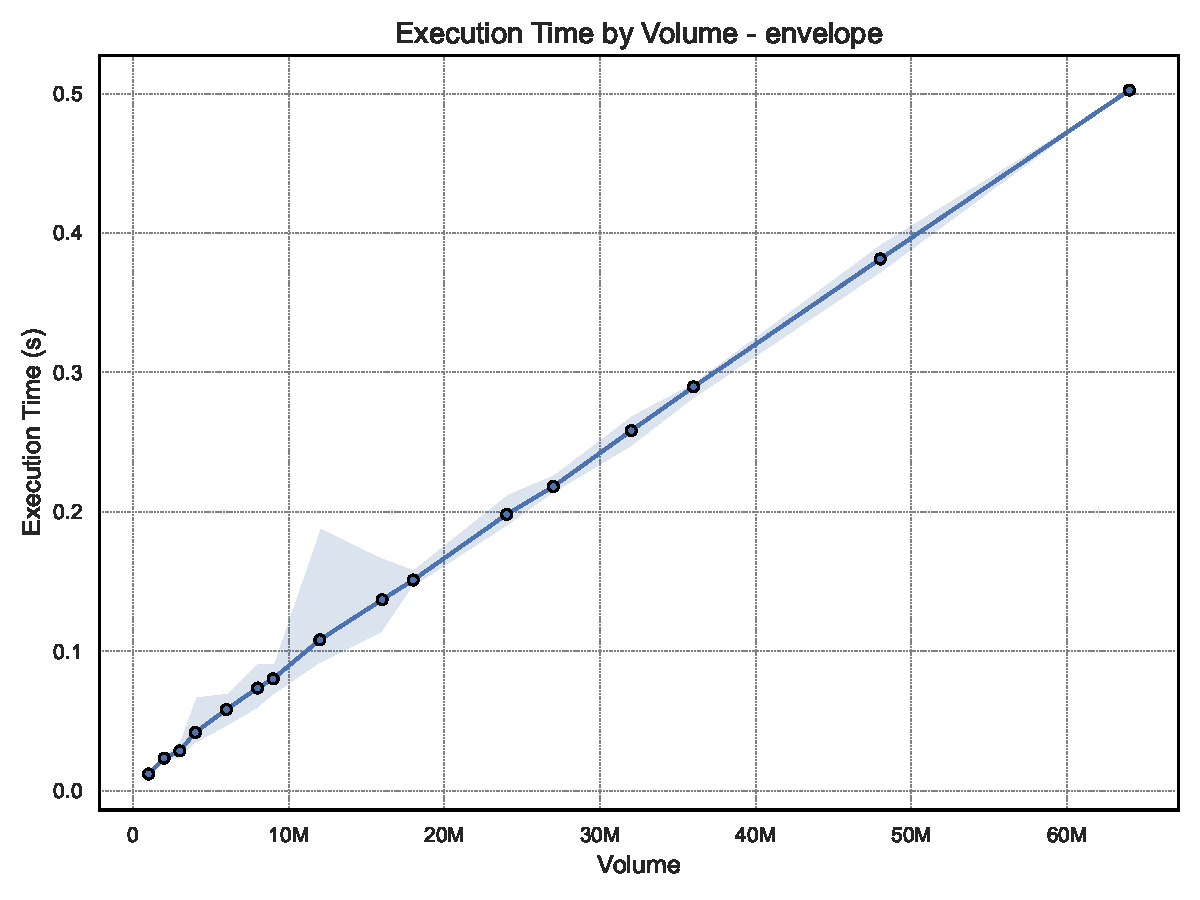
\includegraphics[width=\textwidth]{assets/images/05/execution_time_by_volume_envelope}
    \end{subfigure}
    \hfill
    \begin{subfigure}[t]{0.49\textwidth}
        \centering
        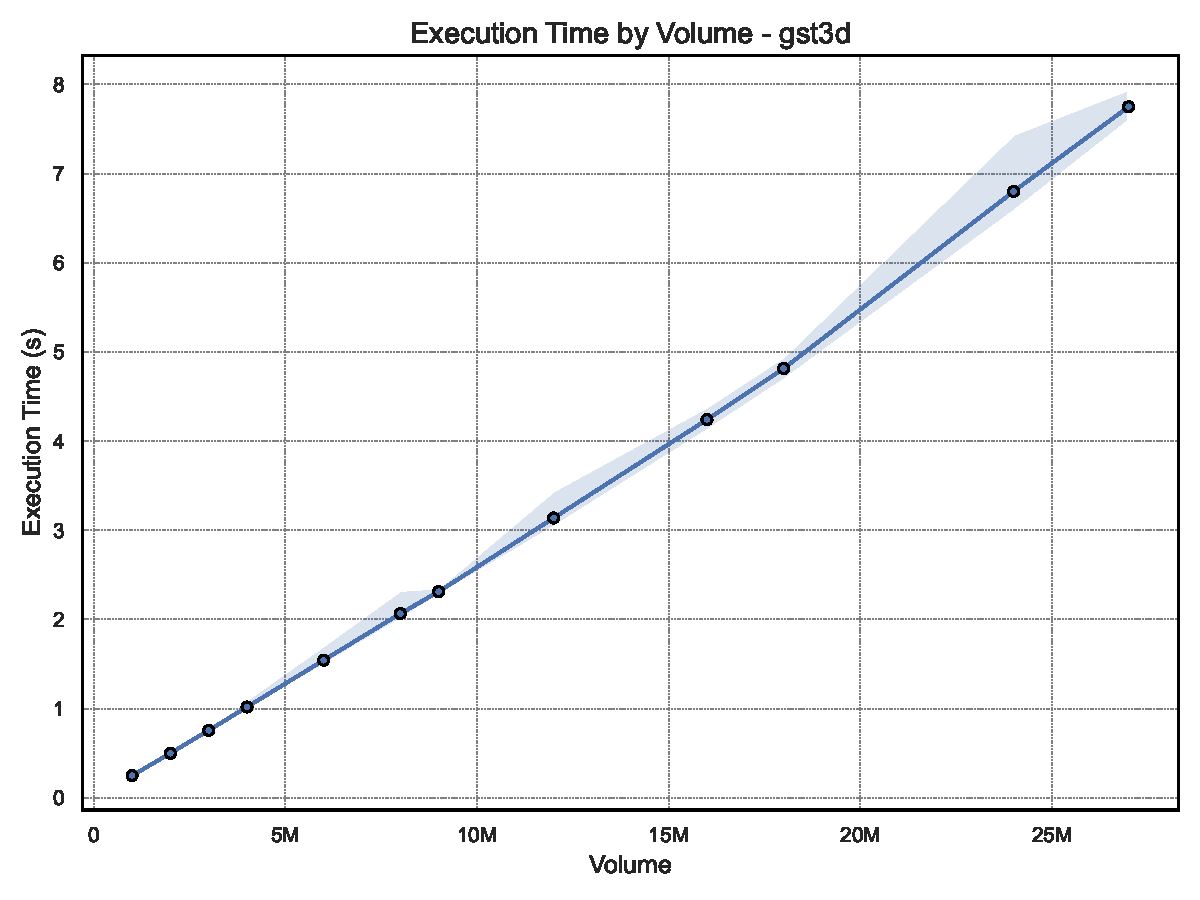
\includegraphics[width=\textwidth]{assets/images/05/execution_time_by_volume_gst3d}
    \end{subfigure}
    \hfill
    \begin{subfigure}[t]{0.49\textwidth}
        \centering
        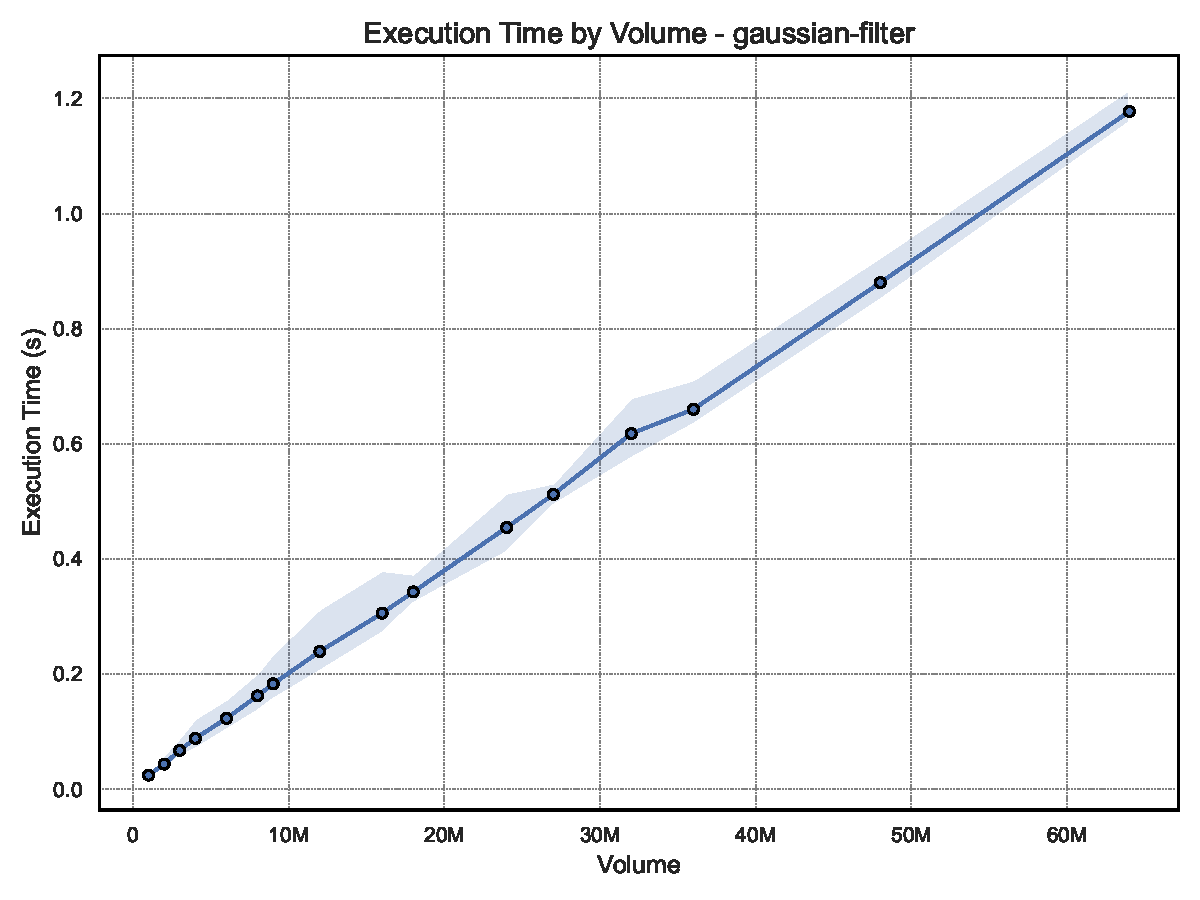
\includegraphics[width=\textwidth]{assets/images/05/execution_time_by_volume_gaussian-filter}
    \end{subfigure}
    \caption{
        Execution time by volume for Envelope, \ac{GST3D}, and Gaussian Filter. 
        All three operators show an increasing trend, reinforcing the impact of volume on processing duration. 
        \label{fig:execution_time_by_volume_facet}
    }
\end{figure*}

\subsection{Execution Time Distributions and Scaling Factor}
\label{subsec:execution-time-distributions-and-scaling}

To complement the volume-based analysis, Figures~\ref{fig:ex_peak_mu_facet}(a)--(b) compare execution time and peak memory usage across all operators.
Both metrics escalate in near-lockstep with input size.
Figure~\ref{fig:ex_peak_mu_facet}(c) then quantifies memory scaling slopes via linear-fits for each operator’s average peak \ac{RAM} usage. 
\EB{Acho que fica melhor mostrar o slope da regressão linear em uma tabela - você poderia mostrar o $R^2$ também. Isso tornadria o gráfico menor e talvez passível de inserção logo após o parágrafo que referencia ele.}
\ac{GST3D} stands out for having the highest slope, suggesting it holds more intermediate data structures during discontinuity detection.
Envelope lies in the middle, while Gaussian Filter’s slope is relatively smaller, implying that it processes data blocks \EBC{more incrementally}{o que quer dizer de forma mais incremental? seria por partes? Mas todos eles não realizam o cálculo por partes? i.e., por chunks?}.

\begin{figure*}[htbp]
    \centering
    \begin{subfigure}[t]{0.49\textwidth}
        \centering
        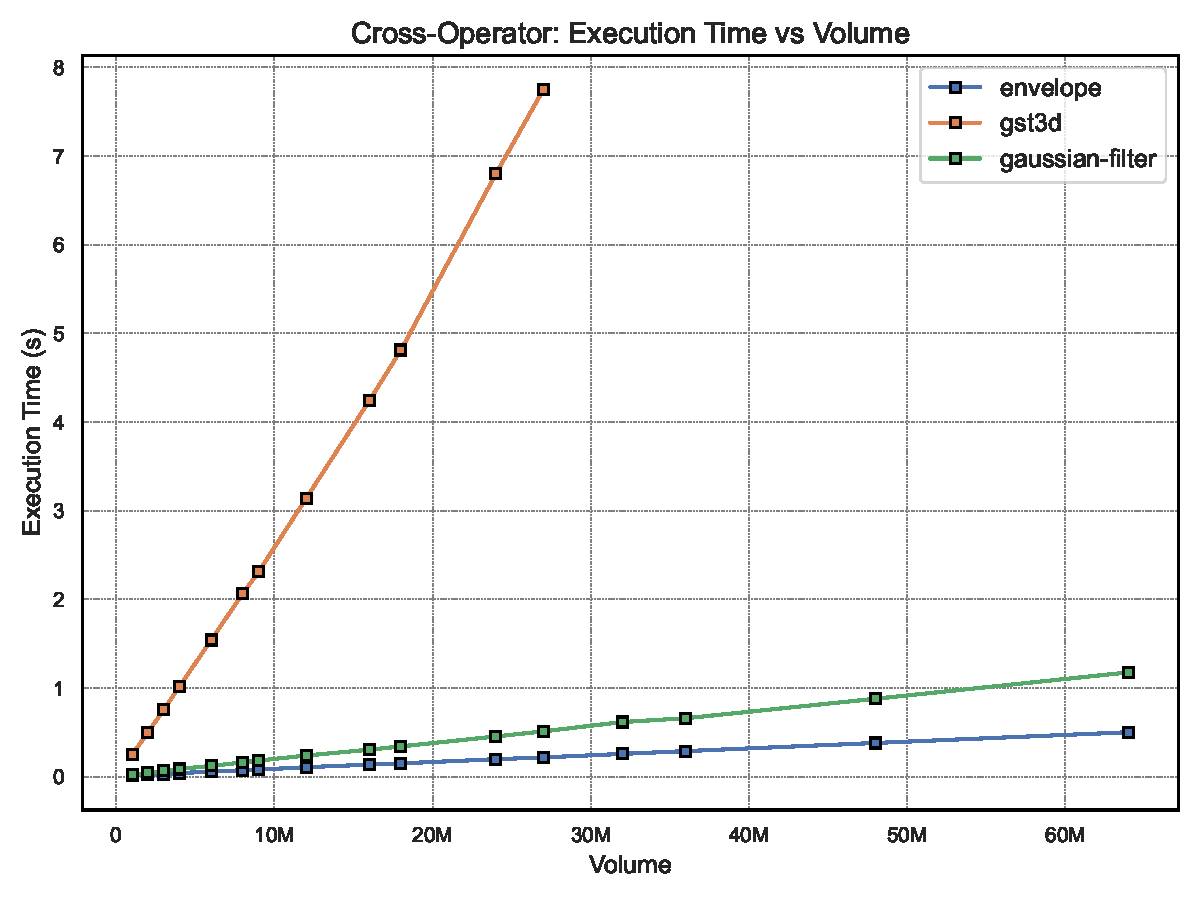
\includegraphics[width=\textwidth]{assets/images/05/cross_execution_time_by_volume}
        \caption{Execution time vs. volume for all three operators.}
    \end{subfigure}
    \hfill
    \begin{subfigure}[t]{0.49\textwidth}
        \centering
        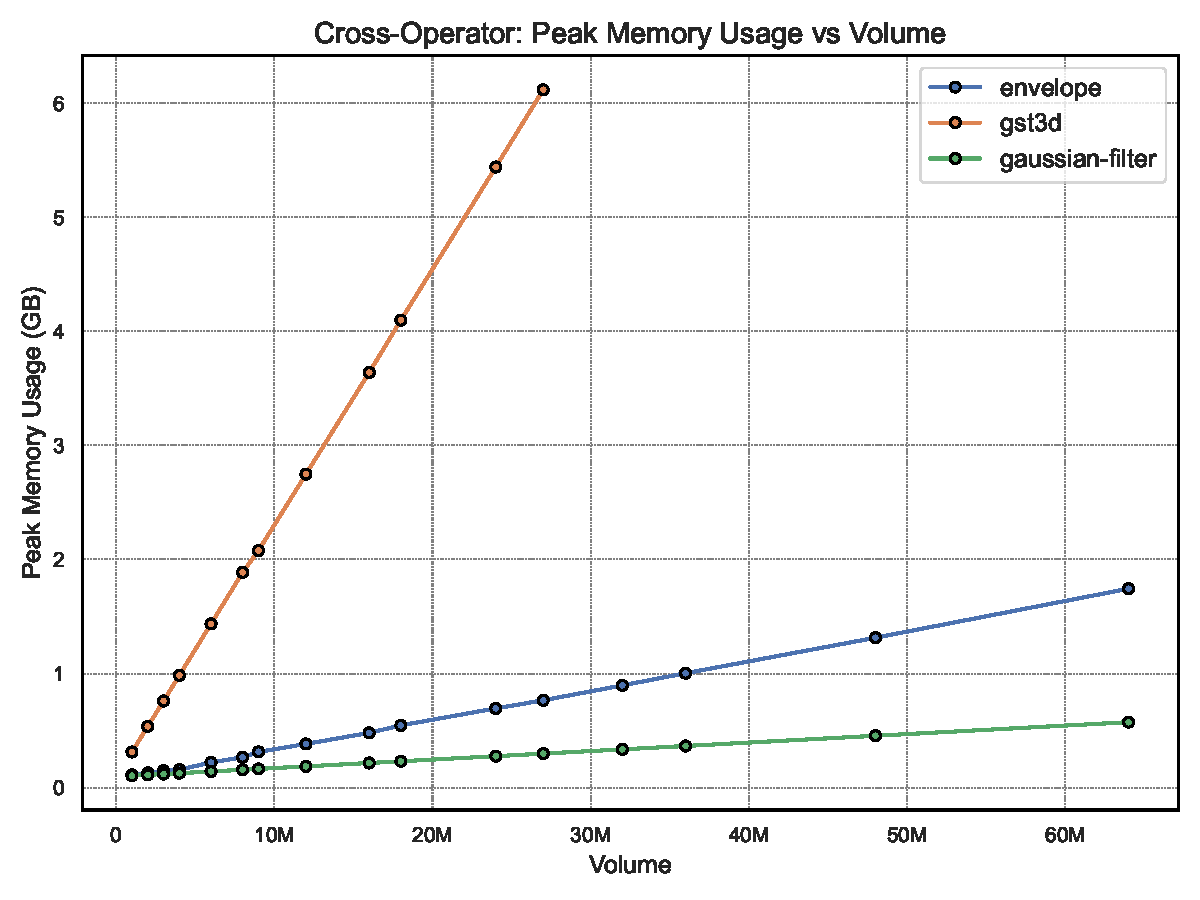
\includegraphics[width=\textwidth]{assets/images/05/cross_peak_memory_by_volume}
        \caption{Peak memory usage vs. volume for all three operators.}
    \end{subfigure}
    \hfill
    \begin{subfigure}[t]{0.49\textwidth}
        \centering
        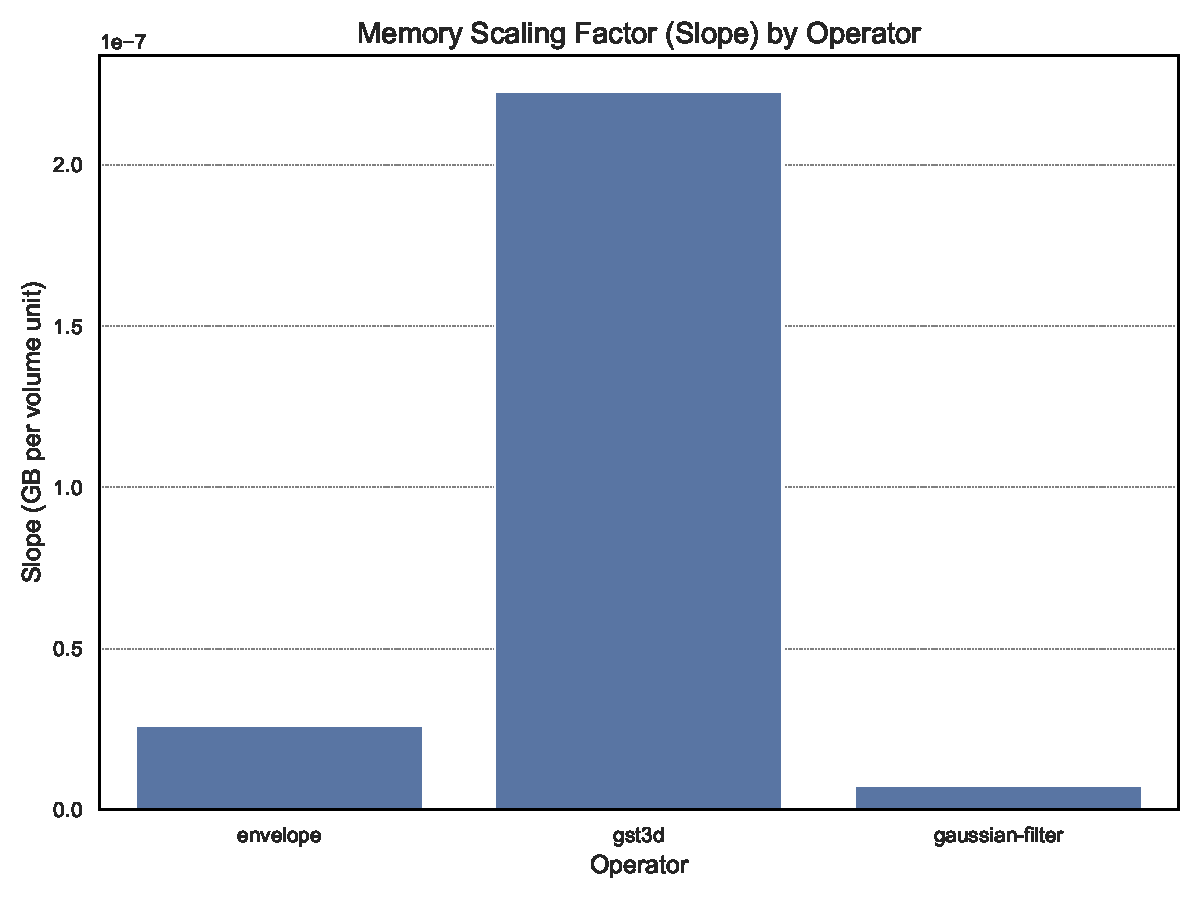
\includegraphics[width=\textwidth]{assets/images/05/cross_operator_memory_scaling_factor}
        \caption{
            Linear-fit slope values (GB/volume). Higher values indicate more pronounced memory growth.
            \EB{Como coloquei no texto, talvez fique melhor remover este gráfico daqui e colocar a informação em uma tabela.}
        }
    \end{subfigure}
    \caption{Combined view of execution time and peak memory usage by volume, and a bar chart revealing the linear-fit slopes for Envelope, \ac{GST3D}, and Gaussian Filter. \ac{GST3D} uses memory most aggressively, while Gaussian Filter is comparatively more memory efficient.}
    \label{fig:ex_peak_mu_facet}
\end{figure*}

In addition, the run durations exhibit right-skewed behavior (Figure~\ref{fig:execution_time_distribution_facet}), consistent with gamma- or lognormal-like distributions. \EB{Este gráfico mostra o histograma do tempo de execução de todos os experimentos? Variando o tamanho do dado? Se sim, a distribuição de tempo de execução tem uma relação mais forte com a seleção das amostras (tamanhos) do que com ruído no sistema, certo?}
While most executions concentrate in the lower range, occasional runs can be significantly longer.
Such tails are not unexpected in \ac{HPC} environments, where system-level noise or particular dataset structures can cause prolonged I/O or memory allocation overhead.
\EB{Não está claro pra mim como este gráfico e estes resultados de tempo contribuem para as principais conclusões derivadas neste capítulo. É interessante ter uma noção do tempo de execução, até mesmo para saber o custo de ser realizar estes experimentos e/ou coletar dados para treinar os modelos, mas além deste ponto, não sei se uma análise de correlação de features e/ou consumo de memória com o tempo de execução está dando suporte aos principais argumentos ou poluindo o capítulo.}

\begin{figure*}[htbp]
    \centering
    \begin{subfigure}[t]{0.49\textwidth}
        \centering
        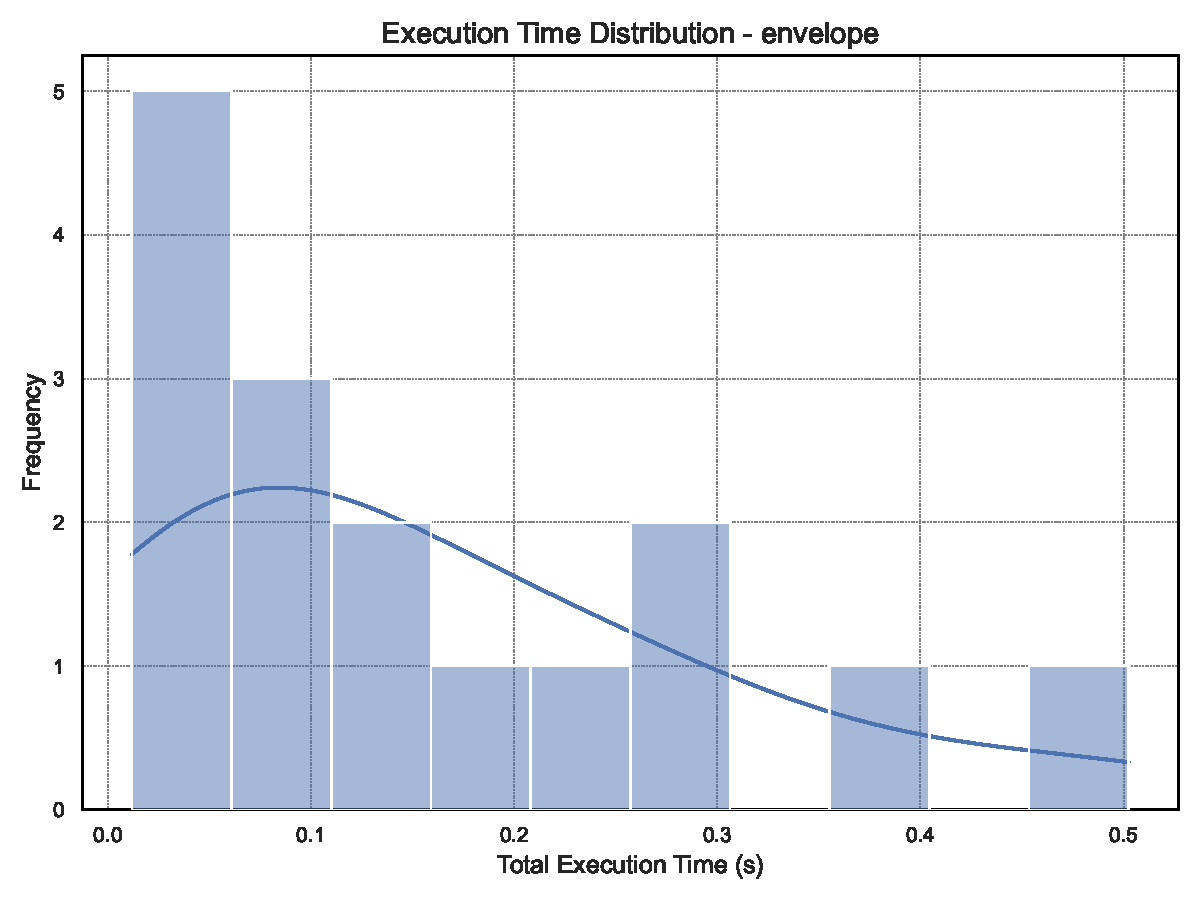
\includegraphics[width=\textwidth]{assets/images/05/execution_time_distribution_envelope}
    \end{subfigure}
    \hfill
    \begin{subfigure}[t]{0.49\textwidth}
        \centering
        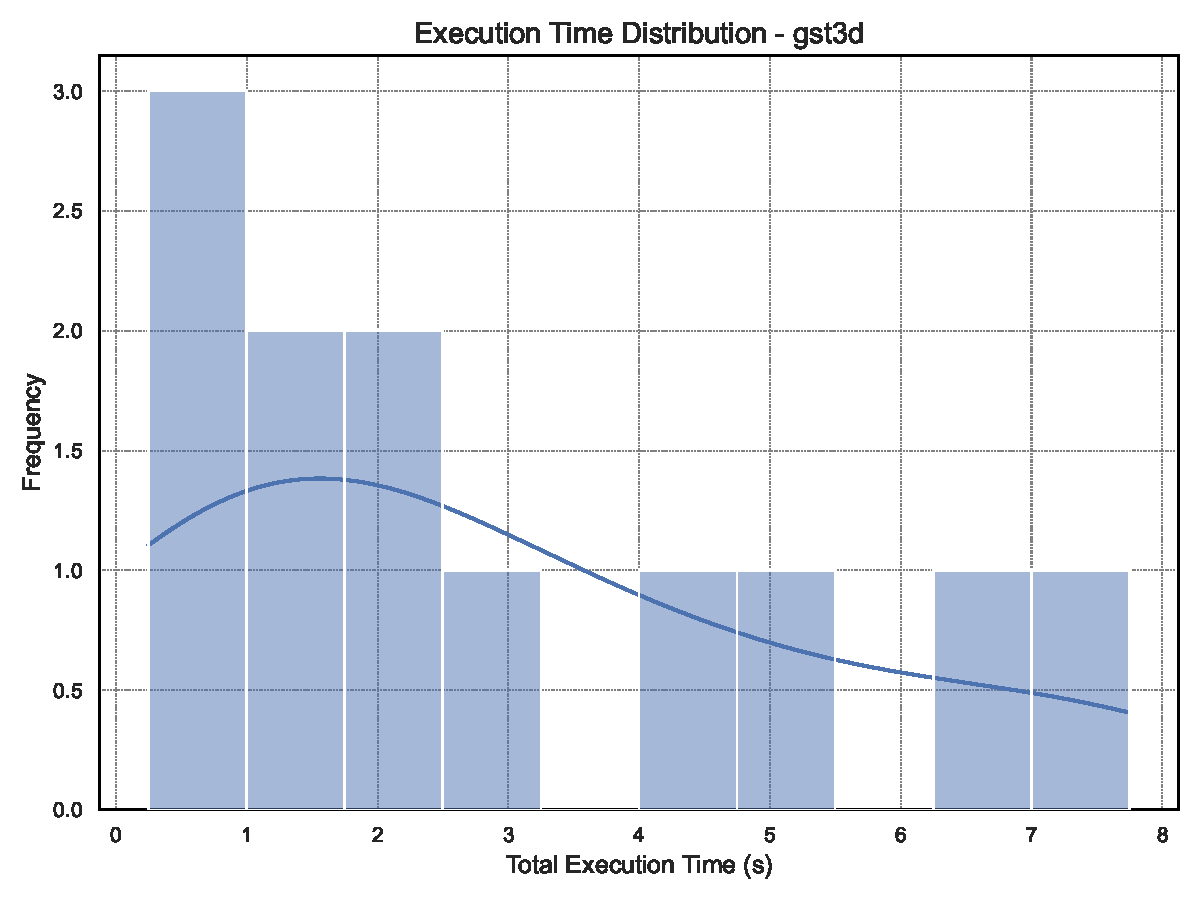
\includegraphics[width=\textwidth]{assets/images/05/execution_time_distribution_gst3d}
    \end{subfigure}
    \hfill
    \begin{subfigure}[t]{0.49\textwidth}
        \centering
        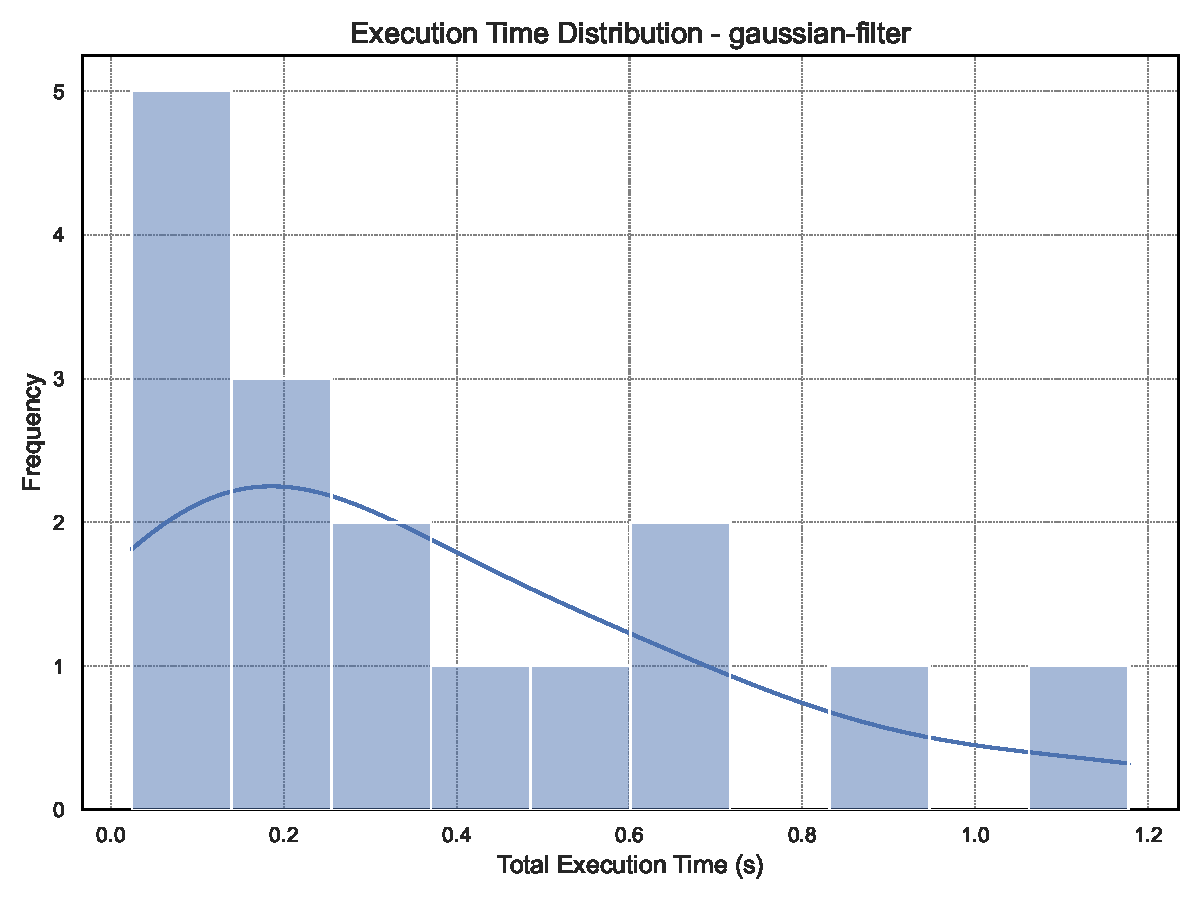
\includegraphics[width=\textwidth]{assets/images/05/execution_time_distribution_gaussian-filter}
    \end{subfigure}
    \caption{Execution time distributions for Envelope, \ac{GST3D}, and the Gaussian Filter. Each distribution displays a heavy right tail, indicating that while most runs finish quickly, certain configurations or system conditions can cause notable slowdowns.}
    \label{fig:execution_time_distribution_facet}
\end{figure*}

\subsection{Dimension-Specific and Time-Progression Analysis}
\label{subsec:dimension-specific-and-time-progression-analysis}

\EB{Como mencionei anteriormente, não está claro para mim se esta análise de tempo de execução é muito relevante.}

To better understand how different axes of the seismic volume factor into resource usage, we break down memory usage by \emph{inlines}, \emph{xlines}, and \emph{samples} for the Envelope operator~(Figure~\ref{fig:memory_usage_by_configuration_envelope}).
We observe that each dimension exerts a similar influence on memory consumption; no single dimension overwhelmingly dominates the Envelope’s consumption pattern.
This outcome aligns with the notion that Envelope is an element-wise amplitude calculation, depending uniformly on the size of the entire input array.

\begin{figure*}[htbp]
    \centering
    \begin{subfigure}[t]{0.49\textwidth}
        \centering
        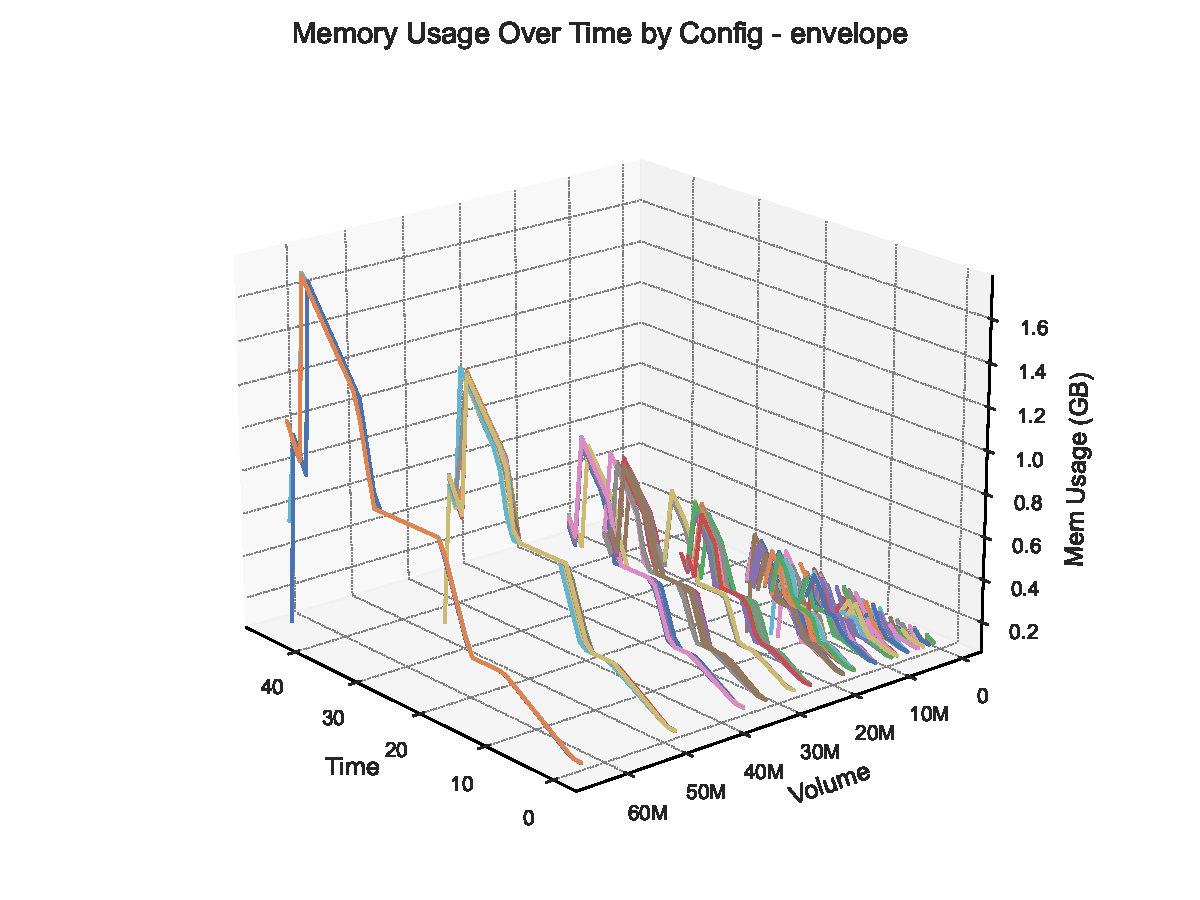
\includegraphics[width=\textwidth]{assets/images/05/memory_usage_by_configuration_envelope}
        \caption{Memory usage binned by individual shape parameters. Each axis increases overall memory similarly.}
    \end{subfigure}
    \hfill
    \begin{subfigure}[t]{0.49\textwidth}
        \centering
        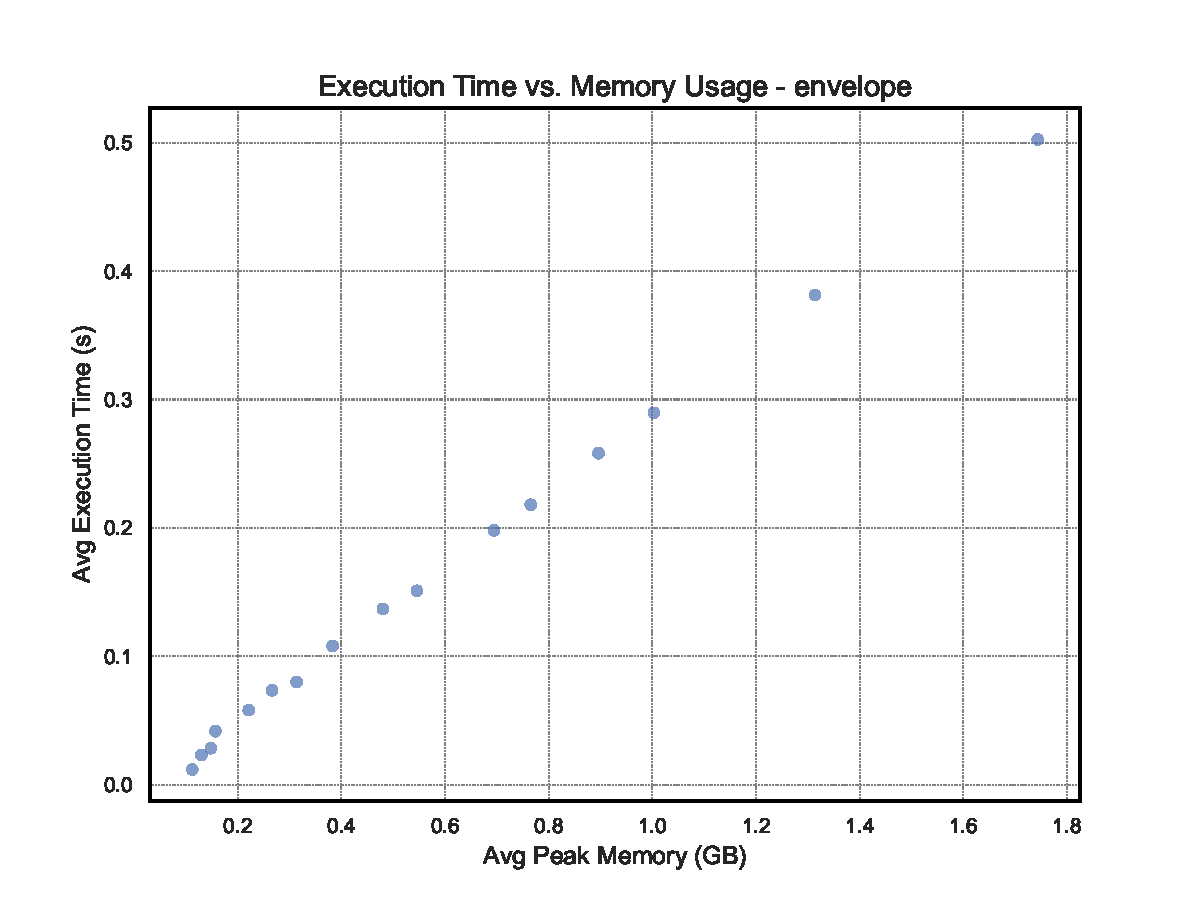
\includegraphics[width=\textwidth]{assets/images/05/execution_time_vs_memory_envelope}
        \caption{Execution time vs. memory usage for Envelope, indicating a mild correlation (longer runs often consume more \ac{RAM}).
            \EB{Não ficou claro para mim como este resultado dá suporte às principais conclusões do capítulo.}
        }
    \end{subfigure}
    \hfill
    \begin{subfigure}[t]{0.49\textwidth}
        \centering
        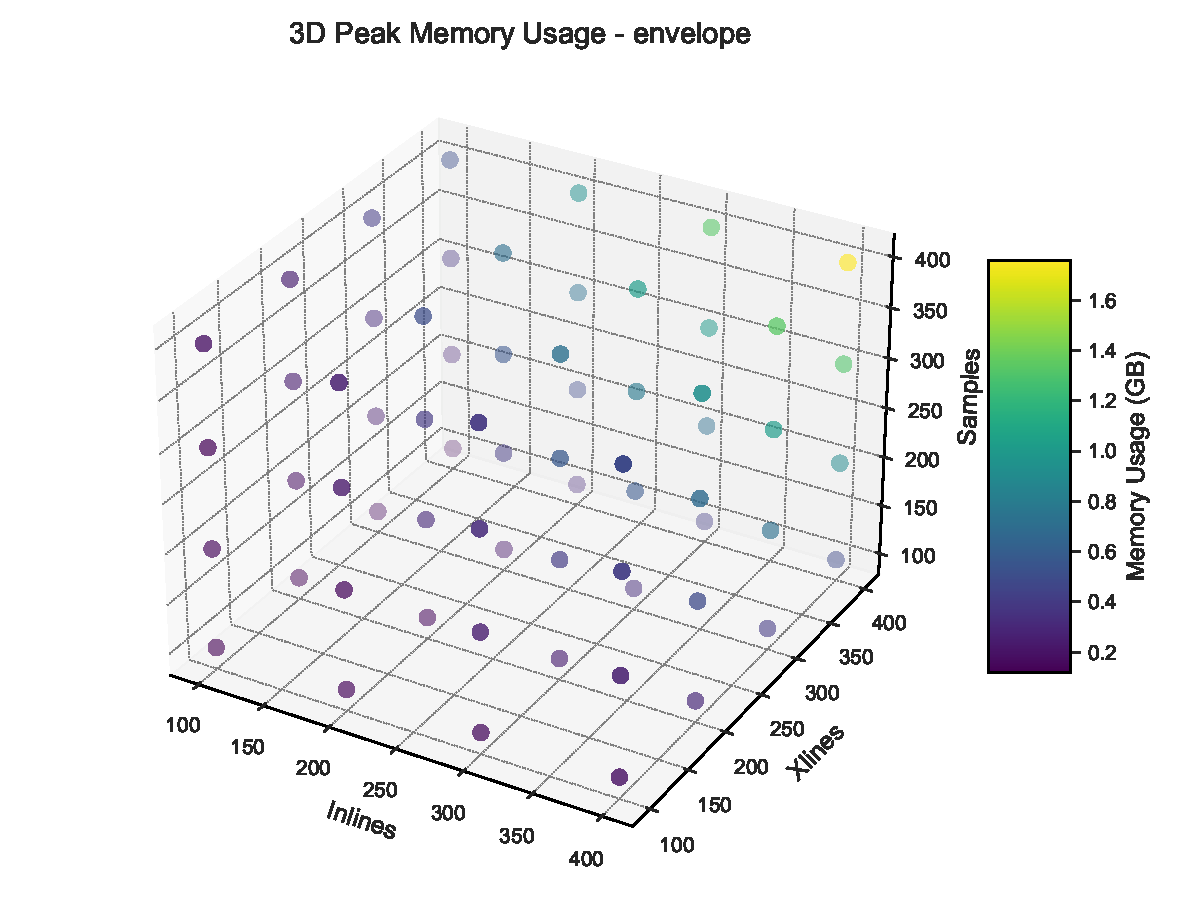
\includegraphics[width=\textwidth]{assets/images/05/memory_usage_inlines_xlines_samples_heatmap_envelope}
        \caption{Heatmap combining inlines, xlines, and samples into a 2D view; warmer colors indicate higher memory usage.
            \EB{Estou inferindo que o objetivo deste gráfico é mostrar que cada dimensão tem uma influência similar no consumo de memória. Se for o caso, acho que seria bom explicar o gráfico no texto e discutir quais características do gráfico levam a esta conclusão.}
        }
    \end{subfigure}
    \caption{Memory usage and runtime analysis for the Envelope operator. 
        All three dimensions appear to scale memory demand in a similar manner, and bigger shapes generally require longer processing times.
        \label{fig:memory_usage_by_configuration_envelope}
    }
\end{figure*}

Figure~\ref{fig:inline_xline_memory_usage_progression_envelope} further highlights how the Envelope operator’s memory usage accumulates over time.
The growth pattern is relatively uniform, aligning with the straightforward element-wise nature of the algorithm.
More complex operators like \ac{GST3D} may reveal steeper or stage-based ramps, particularly if certain algorithmic phases allocate additional buffers or caching mechanisms at specific intervals.
\EB{Qual a principal conclusão (\textit{insight}) que podemos derivar deste experimento?}

\begin{figure}[htbp]
    \centering
    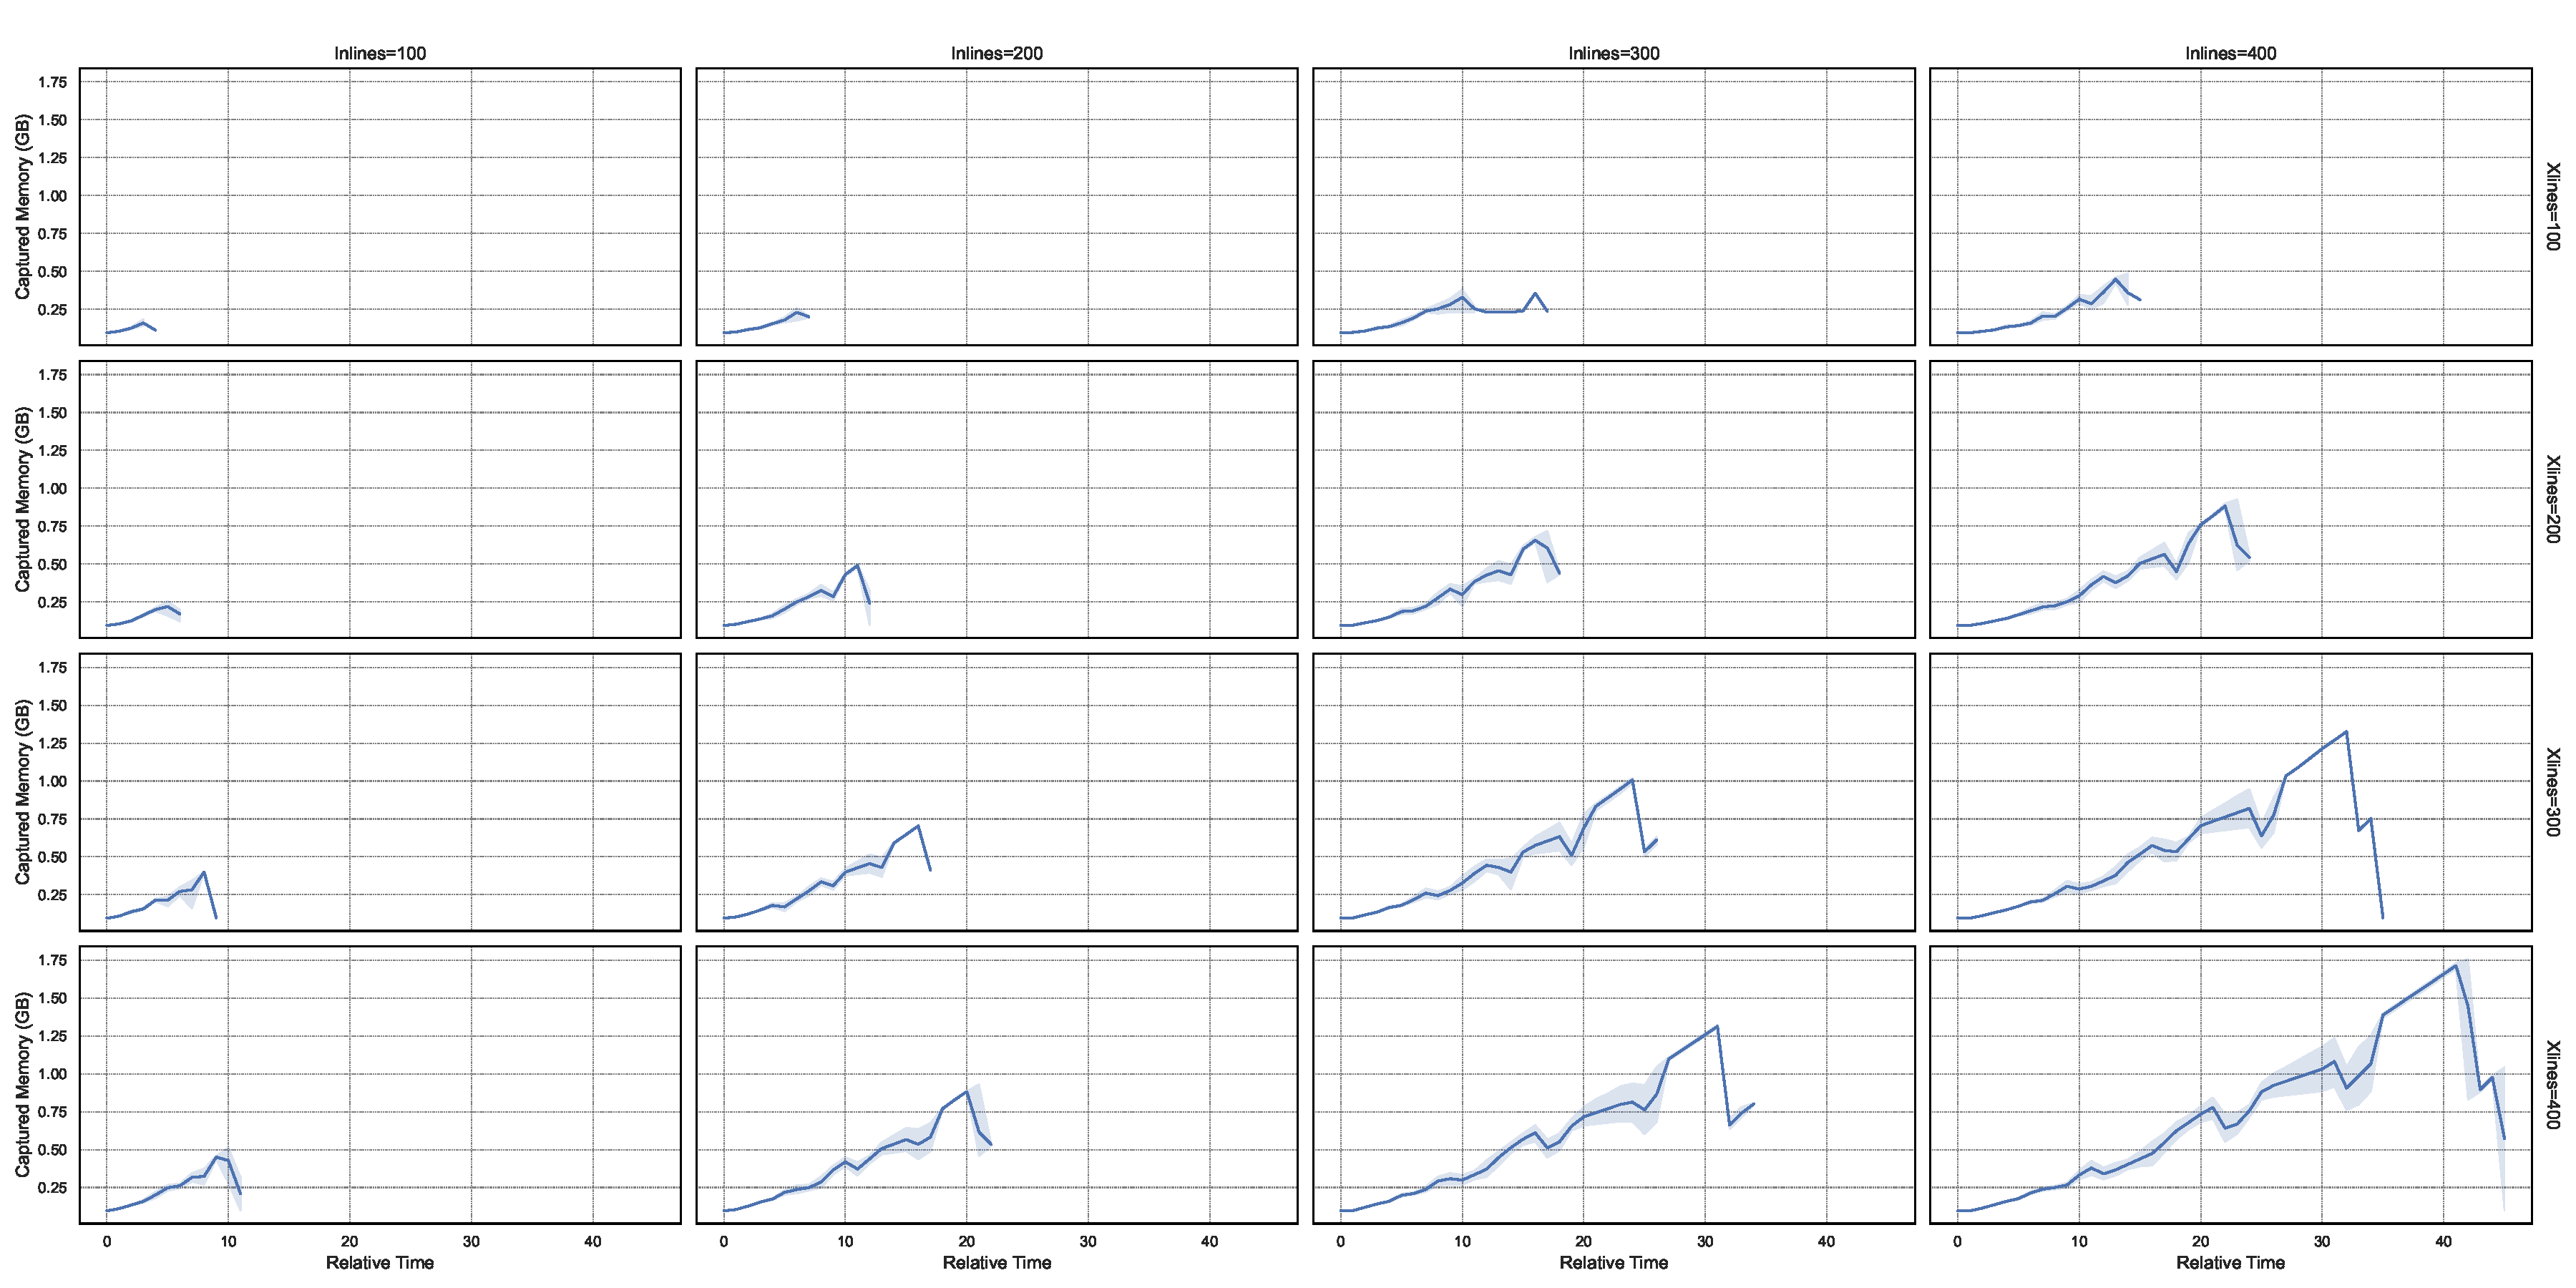
\includegraphics[width=\textwidth]{assets/images/05/inline_xline_memory_usage_progression_envelope}
    \caption{Memory usage progression over time (Envelope operator) for different inlines and xlines. 
        The consumption profile ramps up gradually rather than spiking in distinct phases.
        \label{fig:inline_xline_memory_usage_progression_envelope}
    }
\end{figure}

\subsection{Memory Safety Margins}
\label{subsec:memory-safety-margins}

In real-world \ac{HPC} contexts, underestimating memory can cause abrupt job failures, while overestimation wastes resources.
Figure~\ref{fig:memory_safety_margin} showcases how much peak usage can deviate from average usage by comparing mean and 95th-percentile values.
Envelope and \ac{GST3D} exhibit particularly large deviations for certain volume ranges, hinting that HPC practitioners may need to add a safety buffer beyond the mean consumption to accommodate transient memory spikes.
\EB{Este parágrafo me leva a crer que você está usando a \emph{feature} volume para fazer esta análise. Não seria mais adequado agrupar os dados de acordo com a tupla (inlines, xlines, samples) para evitar que variações de consumo de memória causadas por mudanças nestes valores nos levem a concluir que o motivo é o sistema? P.ex., a tupla (10, 10, 20) pode gerar resultados da tupla (20, 10, 10) que, apesar de terem o mesmo volume, são diferentes.}
\EB{Se tem tanta variação, como foi possível treinar os modelos somente com esta feature e chegar a valores de erro tão pequenos? Os erros não deveriam refletir as variações que observamos aqui?}


\begin{figure*}[htbp]
    \centering
    \begin{subfigure}[t]{0.49\textwidth}
        \centering
        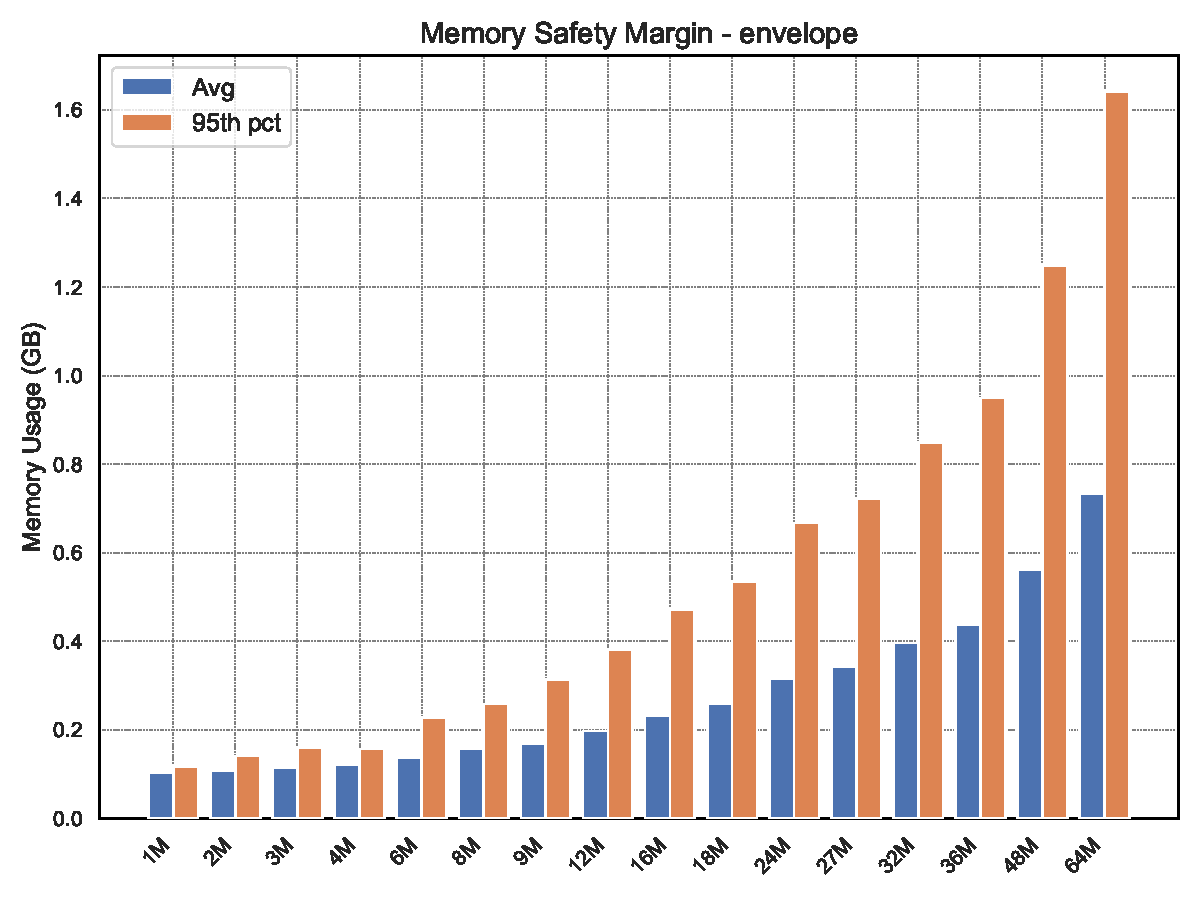
\includegraphics[width=\textwidth]{assets/images/05/memory_safety_margin_envelope}
    \end{subfigure}
    \hfill
    \begin{subfigure}[t]{0.49\textwidth}
        \centering
        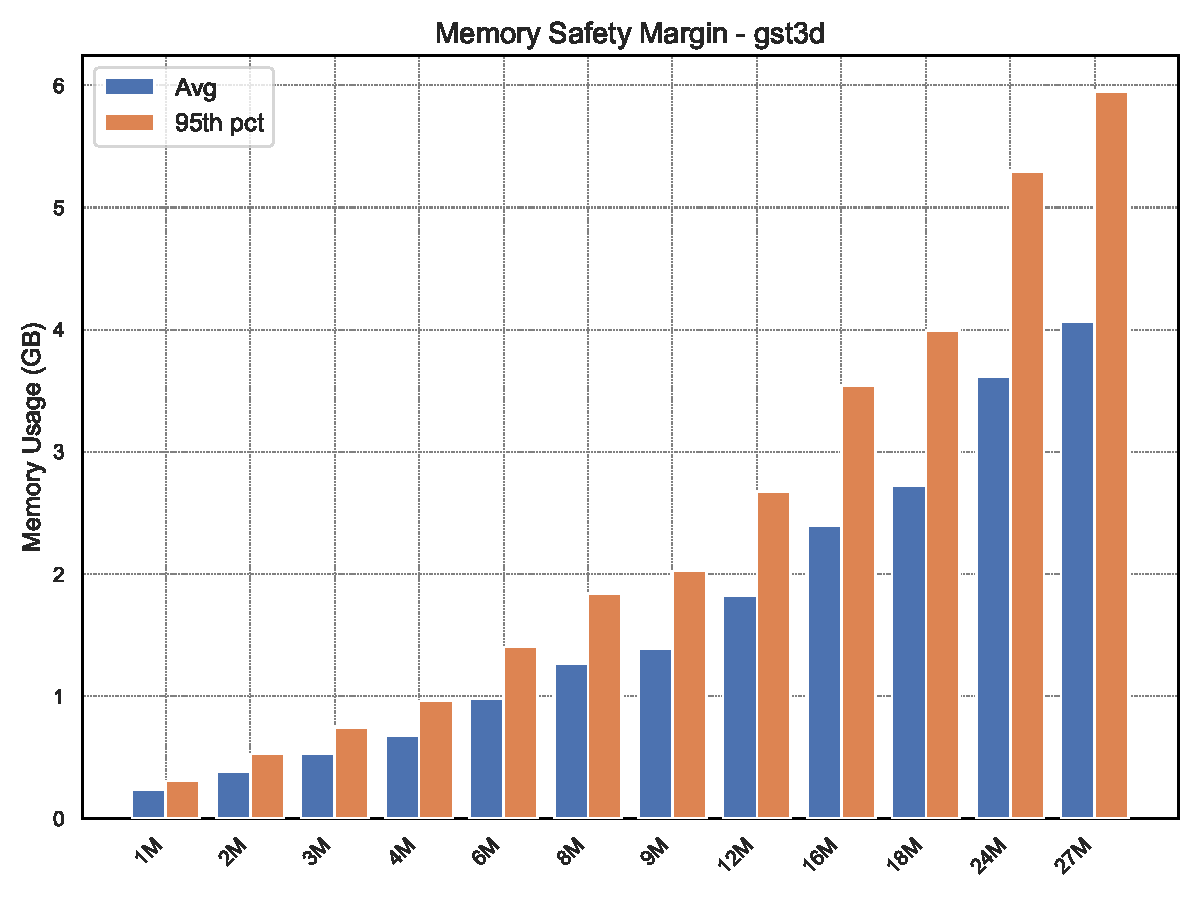
\includegraphics[width=\textwidth]{assets/images/05/memory_safety_margin_gst3d}
    \end{subfigure}
    \hfill
    \begin{subfigure}[t]{0.49\textwidth}
        \centering
        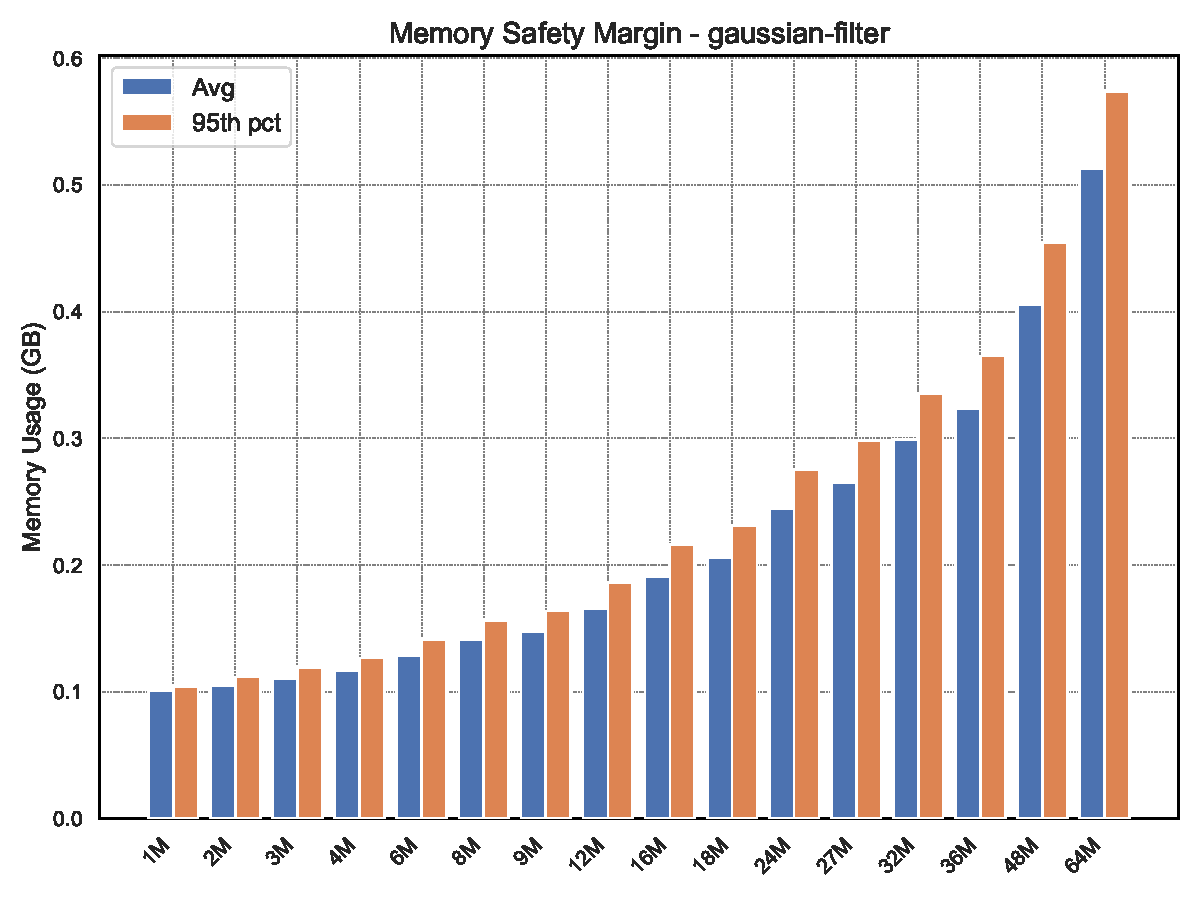
\includegraphics[width=\textwidth]{assets/images/05/memory_safety_margin_gaussian-filter}
    \end{subfigure}
    \caption{Memory safety margins for Envelope, \ac{GST3D}, and the Gaussian Filter. The 95th-percentile often surpasses mean usage by a noticeable margin, revealing the unpredictability of peak memory events.}
    \label{fig:memory_safety_margin}
\end{figure*}

These outliers can arise from transient allocation bursts, system-level scheduling, or overhead fluctuations.
Even with container-based isolation, kernel-level memory management can introduce sporadic spikes.
Recognizing these high-percentile events is critical for designing robust pre-runtime memory estimators.
If left unaccounted for, such transient peaks could lead to underestimation, especially for borderline volumes.

\EB{Este me parece ser uma seção bem importante, já que ela discute a questão da margem de erro que devemos levar em consideração na avaliação dos modelos. Quando trabalhamos com os modelos estamos utilizando dados baseados na média ou no 95\%?} 
\EB{Para refletir: Será que não deveríamos estar usando os dados crus, e monitorar estas variações nos errors?}

\EB{BTW, esta variabilidade é usada no cálculo do score que você menciona nas seções subsequentes?}

\subsection{Dimension Correlations}
\label{subsec:dimension-correlations}

We can further investigate how dimension-specific growth patterns contribute to overall memory usage by plotting pairwise relationships between memory usage and the three shape parameters.
Figure~\ref{fig:memory_vs_dimensions_pairplot_gst3d} shows that \ac{GST3D}, in particular, has strong positive correlations between each dimension and peak memory.
Meanwhile, dimension--dimension scatter plots sometimes show inverse correlations due to the systematic way shapes were varied (when one axis is large, another might be slightly smaller).
Nevertheless, once all three dimensions expand simultaneously, the net memory usage grows sharply.

\EB{Daniel, não entendi o gráfico. O que significam os pontos azuis e as linhas vermelhas?}

\begin{figure}[htbp]
    \centering
    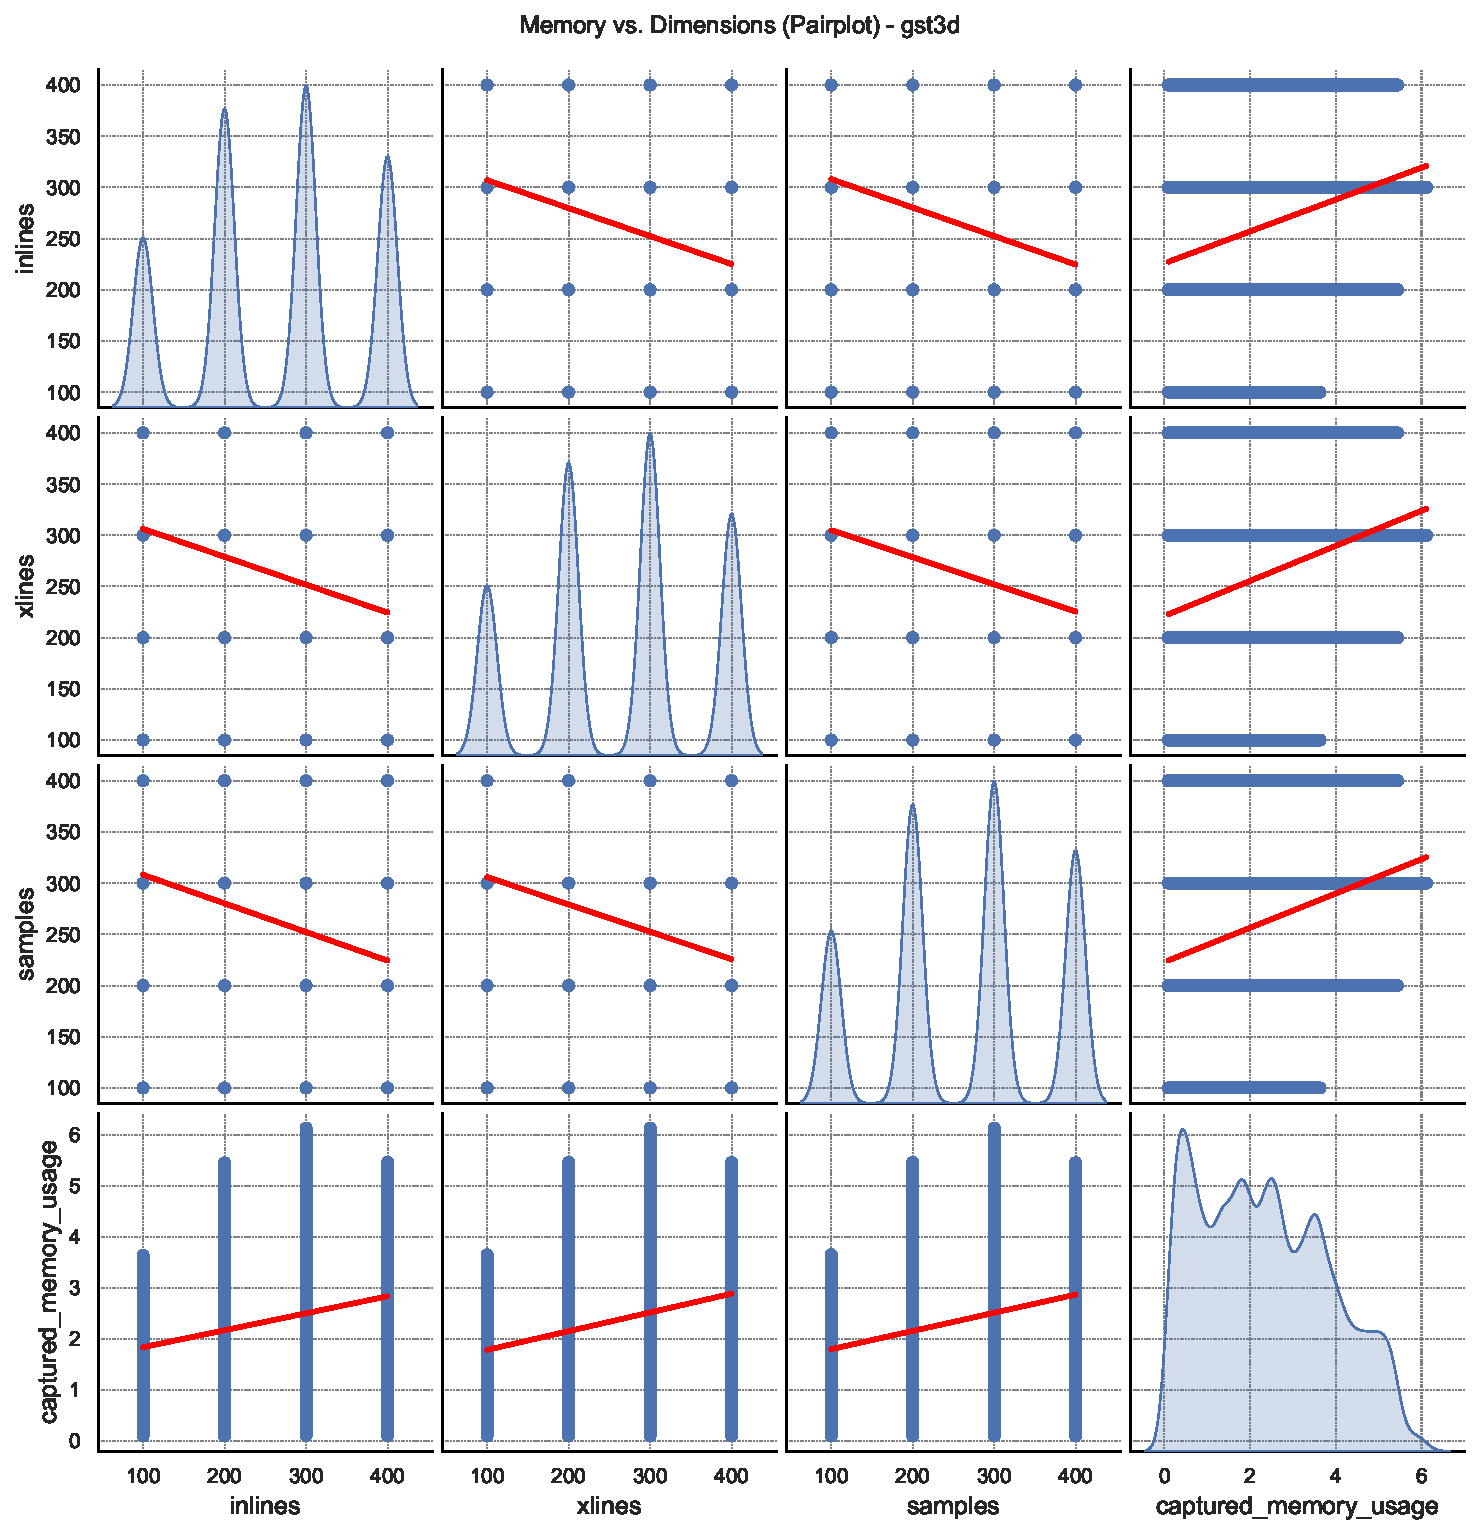
\includegraphics[width=0.9\textwidth]{assets/images/05/memory_vs_dimensions_pairplot_gst3d}
    \caption{Pairplot for \ac{GST3D} memory usage against inlines, xlines, and samples. Positive slopes in memory-related plots confirm that larger shape parameters escalate the overall memory footprint.}
    \label{fig:memory_vs_dimensions_pairplot_gst3d}
\end{figure}

These pairwise correlations, combined with the linear volume trend, underscore that each dimension matters and that polynomial or interaction-based features can help capture how memory usage evolves in less trivial cases (e.g., operators whose complexity grows nonlinearly along certain axes).
\EB{Não ficou claro para mim como você chegou nesta conclusão.}

\subsection{Summary of Observed Resource Usage}
\label{subsec:resource-usage-summary}

Table~\ref{tab:operator_summary_aggregates} provides a high-level summary of all tested volume ranges, memory usage spans, and measured execution times for each operator.
It highlights how, for similarly sized volumes, \ac{GST3D} consistently demands the greatest \EBADD{amount of} \ac{RAM}, with Envelope requiring intermediate amounts, and Gaussian Filter at the lower end (though still significant).
Processing times echo these patterns, with more complex or data-hungry operations tending to take longer.

\begin{table}[htbp]
    \centering
    \begin{tabular}{lcccc}
        \hline
        \textbf{Operator} & \textbf{Volume Range} & \textbf{Peak Mem. Usage (GB)} & \textbf{Exec. Time (s)} \\ \hline
        Envelope &
        $10^6 \!\to\! 6.4\times10^7$ &
        0.10 -- 1.76 &
        0.0106 -- 0.5025 \\
        \ac{GST3D} &
        $10^6 \!\to\! 2.7\times10^7$ &
        0.31 -- 6.12 &
        0.2475 -- 7.75 \\
        Gaussian Filter &
        $10^6 \!\to\! 6.4\times10^7$ &
        0.10 -- 0.57 &
        0.0232 -- 1.22 \\
        \hline
    \end{tabular}
    \caption{Resource usage summary for Envelope, \ac{GST3D}, and Gaussian Filter.
    Volumes are specified in number of elements (e.g., $100 \times 100 \times 100 = 10^6$).
    Memory usage is in GB and time is in seconds.
    Each range denotes the min and max observed across tested volumes.}
    \label{tab:operator_summary_aggregates}
\end{table}

In general, both memory and runtime grow at a near-linear rate, reinforcing the fundamental role of volume in resource demands.
These findings suggest that shape-driven models are likely to be quite effective, especially if they incorporate slight nonlinearities or additional features to handle outliers.
The next sections \EBRPD{delve into}{discuss} how these raw measurements translate into model predictions, discussing which methods and features best capture the trends and variability described above.

\section{Model Performance Overview}
\label{sec:pmc-results-model-performance-overview}

This section analyzes the predictive performance of nine regression models (Linear Regression, Polynomial Regression, Decision Tree, Random Forest, Gradient Boosting, Neural Network, XGBoost, Support Vector Regression, and Elastic Net) when estimating peak memory usage.
Experiments covered Envelope, \ac{GST3D}, and Gaussian Filter operators, each trained and evaluated on the datasets introduced in Section~\ref{subsec:pmc-results-experiment-outputs-overview}.
Multiple performance metrics were computed to offer a comprehensive perspective, including \ac{RMSE}, \ac{MAE}, $R^2$, accuracy (threshold-based), and a \EBC{custom “score” designed to rank models more holistically}{Faltou descrever como este score é calculado e porque ele é importante.}.

\subsection{Cross-Model Comparisons and Key Metrics}
\label{subsec:cross-model-comparisons-and-key-metrics}

Figure~\ref{fig:residual_vs_predicted_and_r2_bar} shows two high-level comparisons across all models and operators.
Part~(a) plots residuals versus predicted values, illustrating that most residuals cluster tightly around zero.
This result signals that many models capture the near-linear trend between \EBC{volume size}{Seria bom deixar claro que neste capítulo você concentra sua análise nesta feature} and memory consumption.
Exceptions arise in \ac{GST3D} runs with the Neural Network model, where residual variance is notably larger.
Part~(b) charts the $R^2$ for each model--operator pair, revealing that Linear Regression, XGBoost, and Elastic Net often top the list.
These results corroborate the idea that relatively simple (or linear-in-spirit) methods work well, given the strong \EBRPD{shape--memory}{data shape--memory consumption} linearity.

\begin{figure*}[htbp]
    \centering
    \begin{subfigure}[t]{0.49\textwidth}
        \centering
        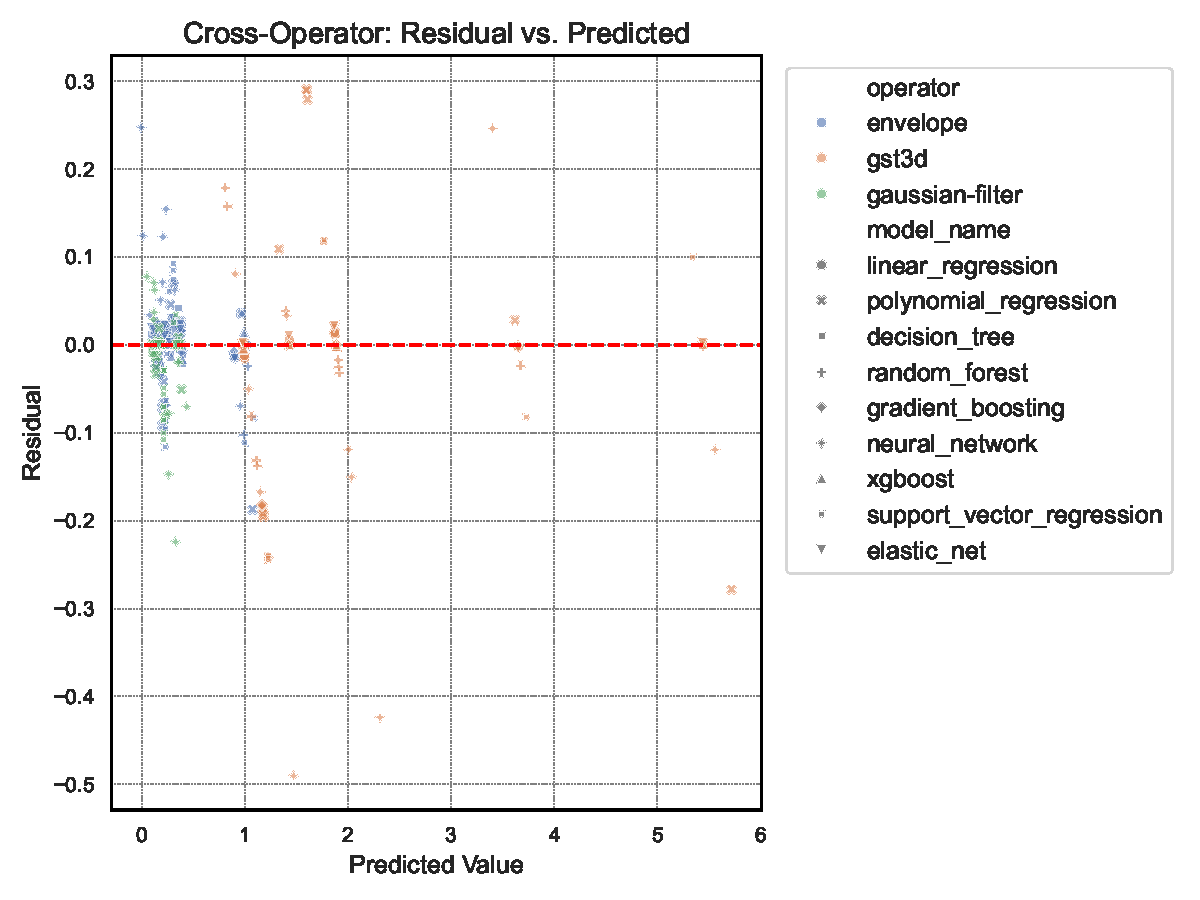
\includegraphics[width=\textwidth]{assets/images/05/residual_vs_predicted}
        \caption{Residual vs.\ predicted values for all operators and models.
            Most models yield low residuals across a wide range of predicted values.
            The \ac{GST3D}–Neural Network pairing stands out for higher errors.
            \EB{Adicione a unidade de medida nos rótulos dos eixos: p.ex.: Residual (GB?) e Predicted Value (GB?)}
        }
    \end{subfigure}
    \hfill
    \begin{subfigure}[t]{0.49\textwidth}
        \centering
        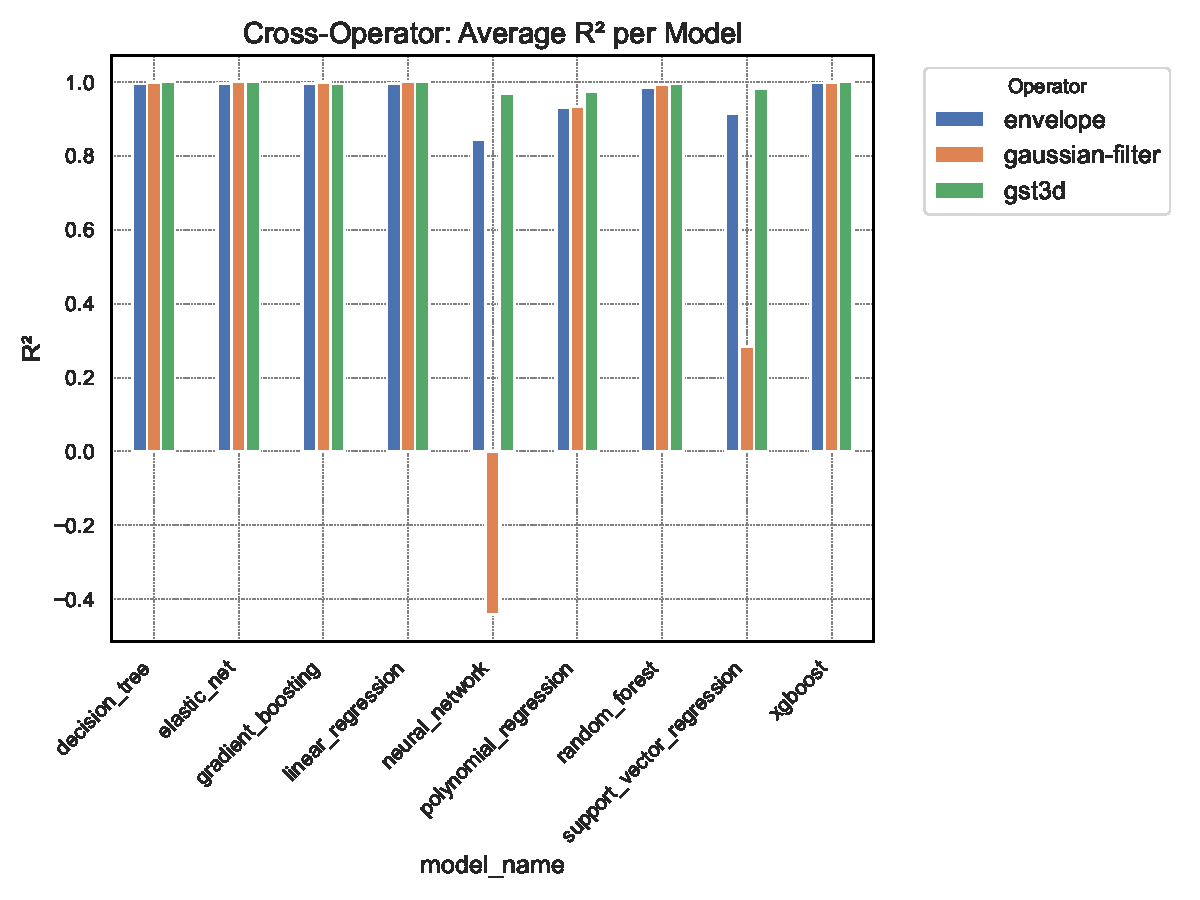
\includegraphics[width=\textwidth]{assets/images/05/cross_model_r2_bar}
        \caption{$R^2$ scores for each model and operator.
        Linear Regression, XGBoost, and Elastic Net perform consistently well.
        The Neural Network underperforms for \ac{GST3D}.}
    \end{subfigure}
    \caption{Overview of cross-model results: (a) residual-versus-predicted scatter plots and (b) $R^2$ bar chart.
        Simpler or regularized linear methods often yield the most stable fits.
        \EB{As fontes destes gráficos estão muito pequenas. Acho que ficaria melhor separar em dois gráficos. Não tenho certeza, mas talvez os dados do gráfico (b) fiquem melhor em uma tabela.}
        \label{fig:residual_vs_predicted_and_r2_bar}
    }
\end{figure*}

Table~\ref{tab:performance_summary} summarizes the main metrics for each operator, aggregated over the nine models.
These data are distilled from the experiment’s \texttt{model\_metrics.csv} files (Envelope, \ac{GST3D}, Gaussian Filter).
The best \EBC{“score”}{definir esta métrica} values for Envelope, \ac{GST3D}, and Gaussian Filter are $2.579$, $2.970$, and $2.904$, respectively.
Gradient Boosting tops Envelope, Decision Tree leads \ac{GST3D}, and Linear Regression narrowly surpasses Elastic Net for the Gaussian Filter.

\begin{table}[htbp]
    \centering
    \begin{tabular}{lccc}
        \hline
        \textbf{Operator} & \textbf{Best Model} & \textbf{Best Score} & \textbf{Note}                    \\
        \hline
        Envelope          & Gradient Boosting   & 2.579               & Consistently low RMSE            \\
        \ac{GST3D}        & Decision Tree       & 2.970               & Highest $R^2$, minimal residuals \\
        Gaussian Filter   & Linear Regression   & 2.904               & Ties closely with Elastic Net    \\
        \hline
    \end{tabular}
    \caption{Summary of top-performing models and their best “score” metric across operators.}
    \label{tab:performance_summary}
\end{table}

\subsection{Operator-Specific Model Scores}
\label{subsec:operator-specific-model-scores}

Figures~\ref{fig:score_by_model_operators} and~\ref{fig:best_model_per_operator} break down model \EBC{scores}{definir esta métrica} per operator and highlight the winning algorithm in each category.
The minor differences among the leading models (Gradient Boosting, XGBoost, Decision Tree, and Linear/Elastic Net) suggest that seismic memory usage is comparatively straightforward to learn, likely due to the near-linear volume relationship observed in Section~\ref{sec:pmc-results-memory-and-execution-time-profiling}.

\begin{figure*}[htbp]
    \centering
    \begin{subfigure}[t]{0.32\textwidth}
        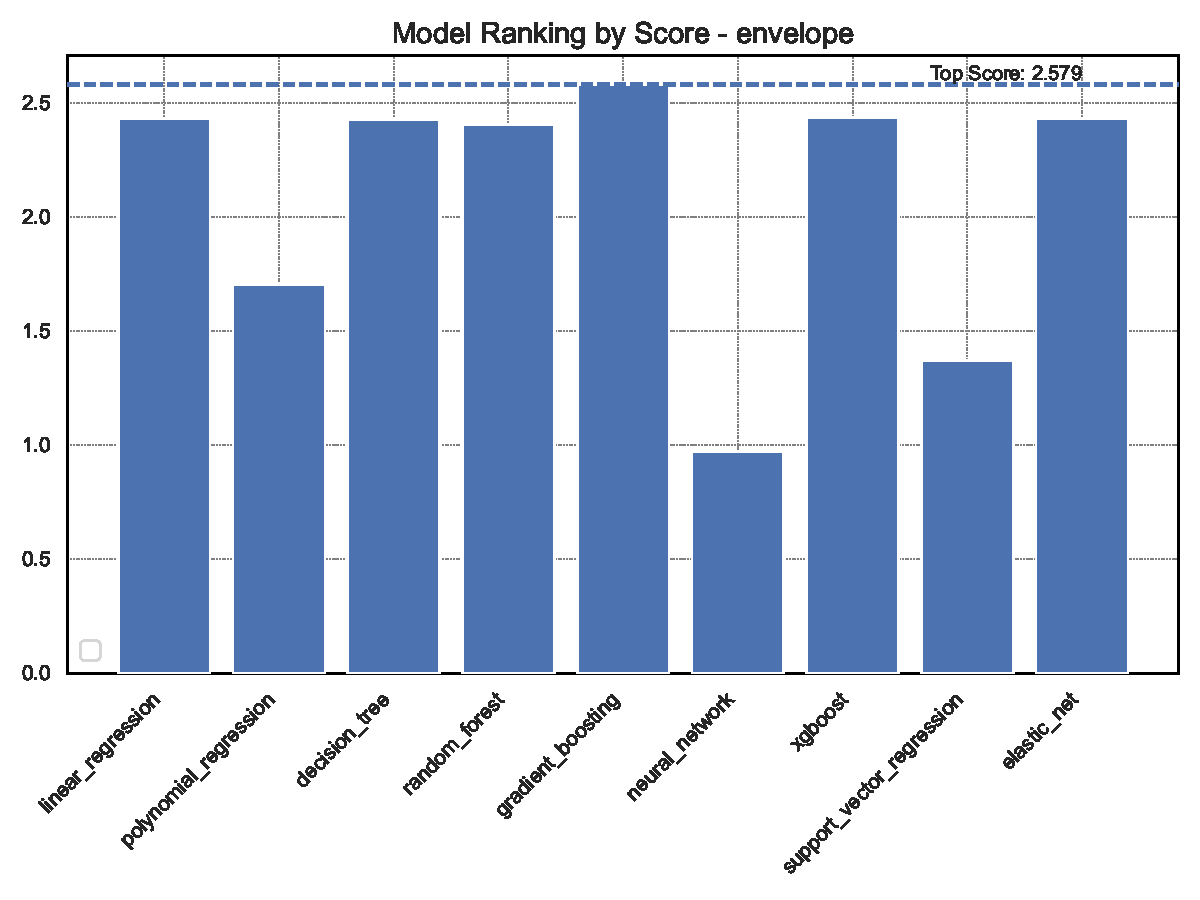
\includegraphics[width=\textwidth]{assets/images/05/score_by_model_envelope}
        \caption{Envelope}
    \end{subfigure}
    \hfill
    \begin{subfigure}[t]{0.32\textwidth}
        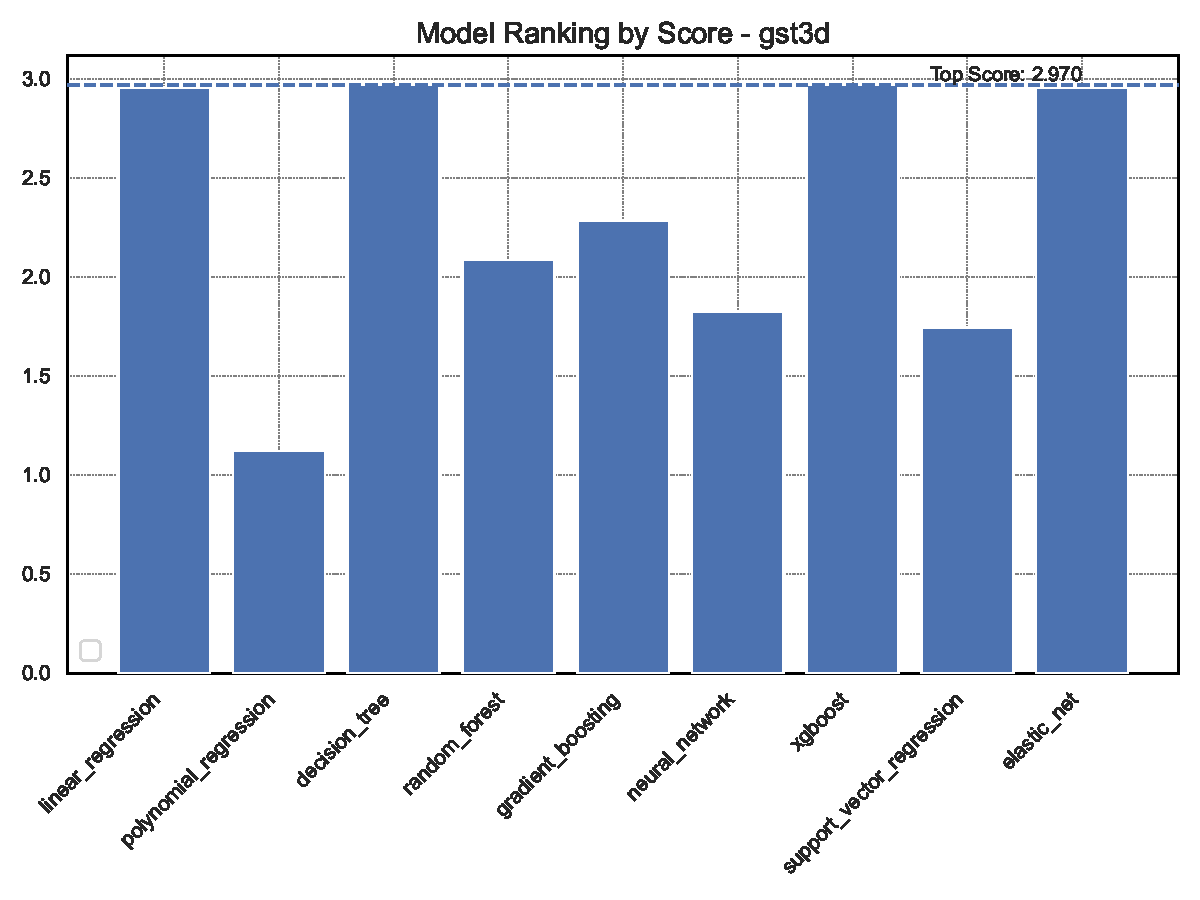
\includegraphics[width=\textwidth]{assets/images/05/score_by_model_gst3d}
        \caption{\ac{GST3D}}
    \end{subfigure}
    \hfill
    \begin{subfigure}[t]{0.32\textwidth}
        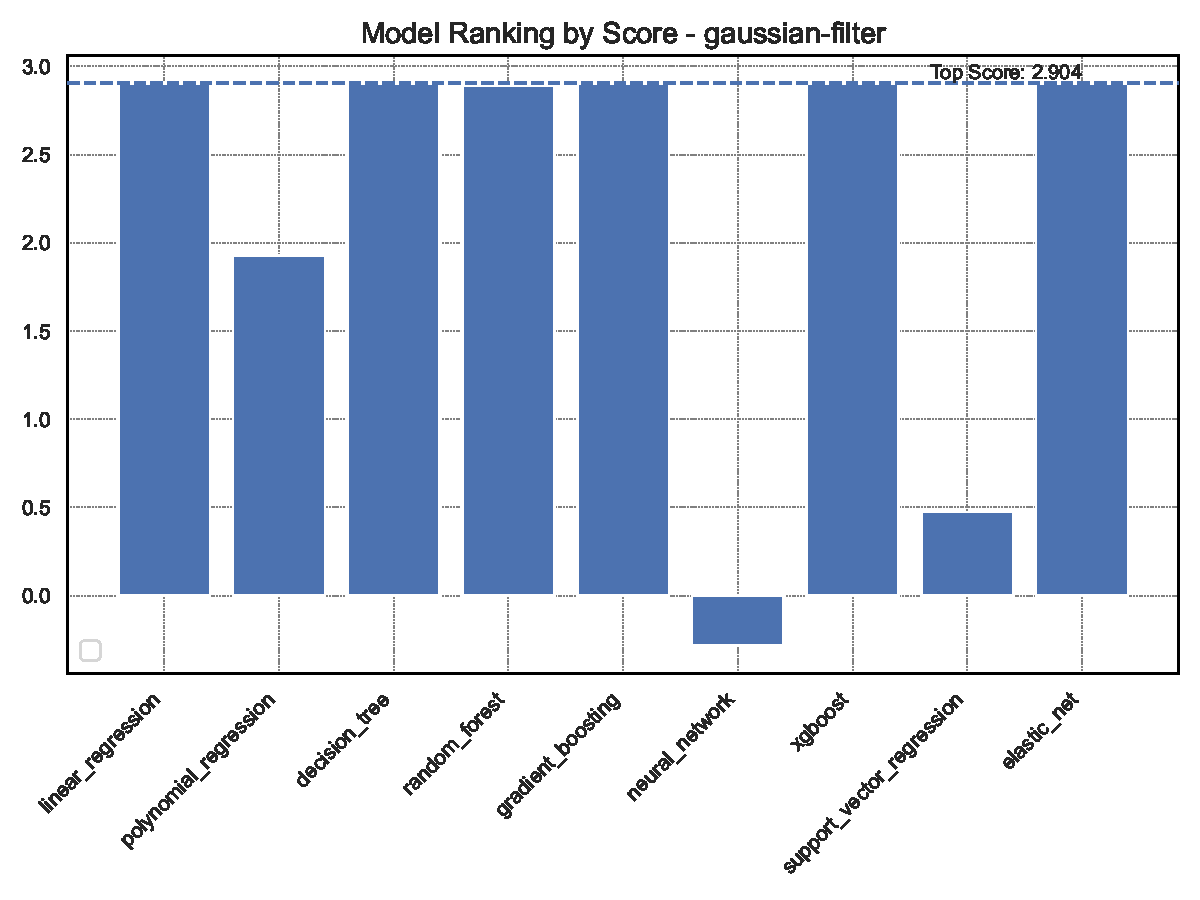
\includegraphics[width=\textwidth]{assets/images/05/score_by_model_gaussian-filter}
        \caption{Gaussian Filter}
    \end{subfigure}
    \caption{\EBC{Scores by model for each operator}{definir a métrica score}.
        A higher score indicates stronger overall performance.
        Multiple models cluster near the top for all three operators, highlighting the relative ease of predicting memory usage from linear shape parameters.
        \label{fig:score_by_model_operators}
    }
\end{figure*}

\begin{figure}[htbp]
    \centering
    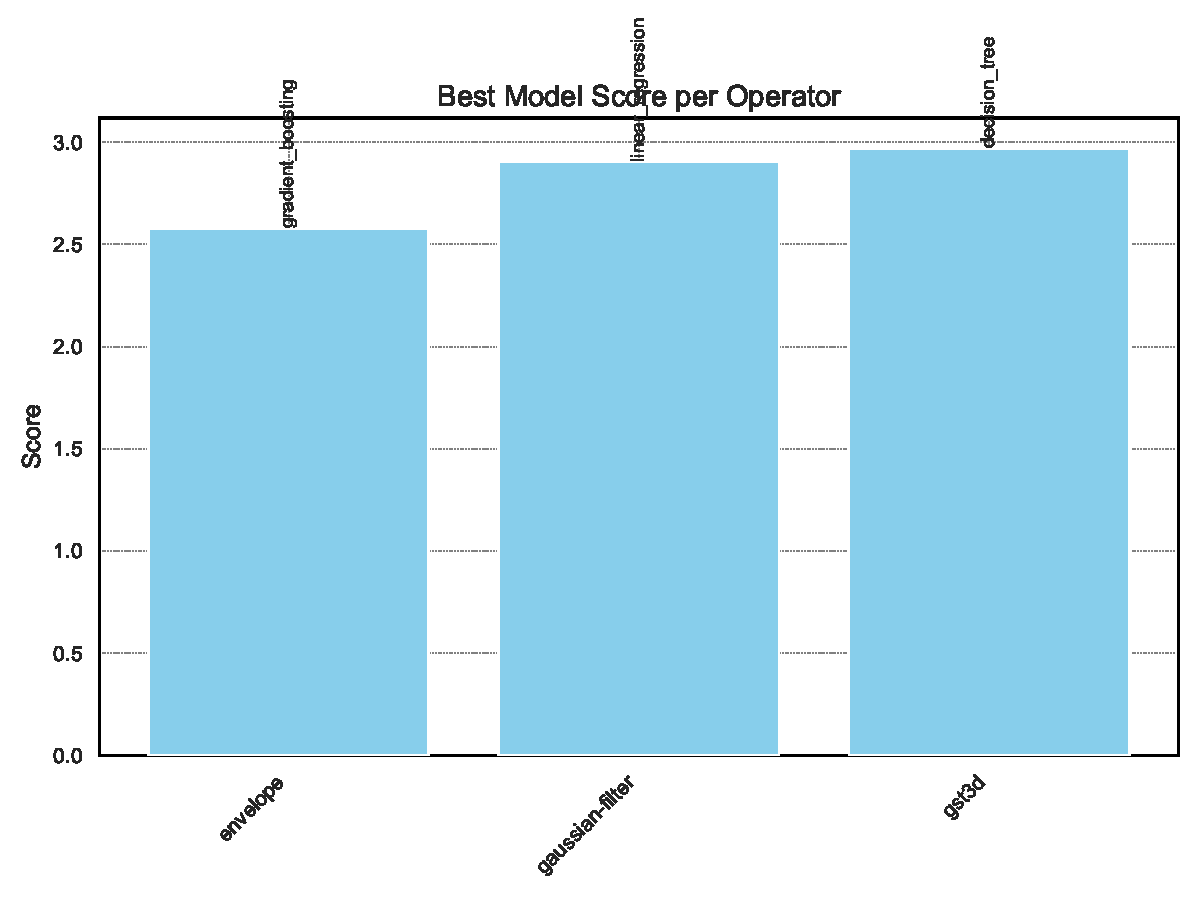
\includegraphics[width=0.6\textwidth]{assets/images/05/best_model_per_operator}
    \caption{Best model per operator by score: Gradient Boosting (Envelope), Decision Tree (\ac{GST3D}), and Linear Regression (Gaussian Filter).
        \EB{Senti falta da definição da métrica "Score"}
        \label{fig:best_model_per_operator}
    }
\end{figure}

\subsection{Accuracy and RMSE Analysis}
\label{subsec:accuracy-and-rmse-analysis}

\EBC{Como você definiu/calculou acurácia?}

Figure~\ref{fig:accuracy_rmse_envelope} illustrates accuracy versus \ac{RMSE} for each model under Envelope, \ac{GST3D}, and Gaussian Filter.
An ideal model would appear near the top-left corner (high accuracy, low \ac{RMSE}).
Polynomial Regression and the Neural Network exhibit relatively higher \ac{RMSE} in \ac{GST3D}, reinforcing the patterns already noted in the residual plots and $R^2$ bars.

\begin{figure*}[htbp]
    \centering
    \begin{subfigure}[t]{0.32\textwidth}
        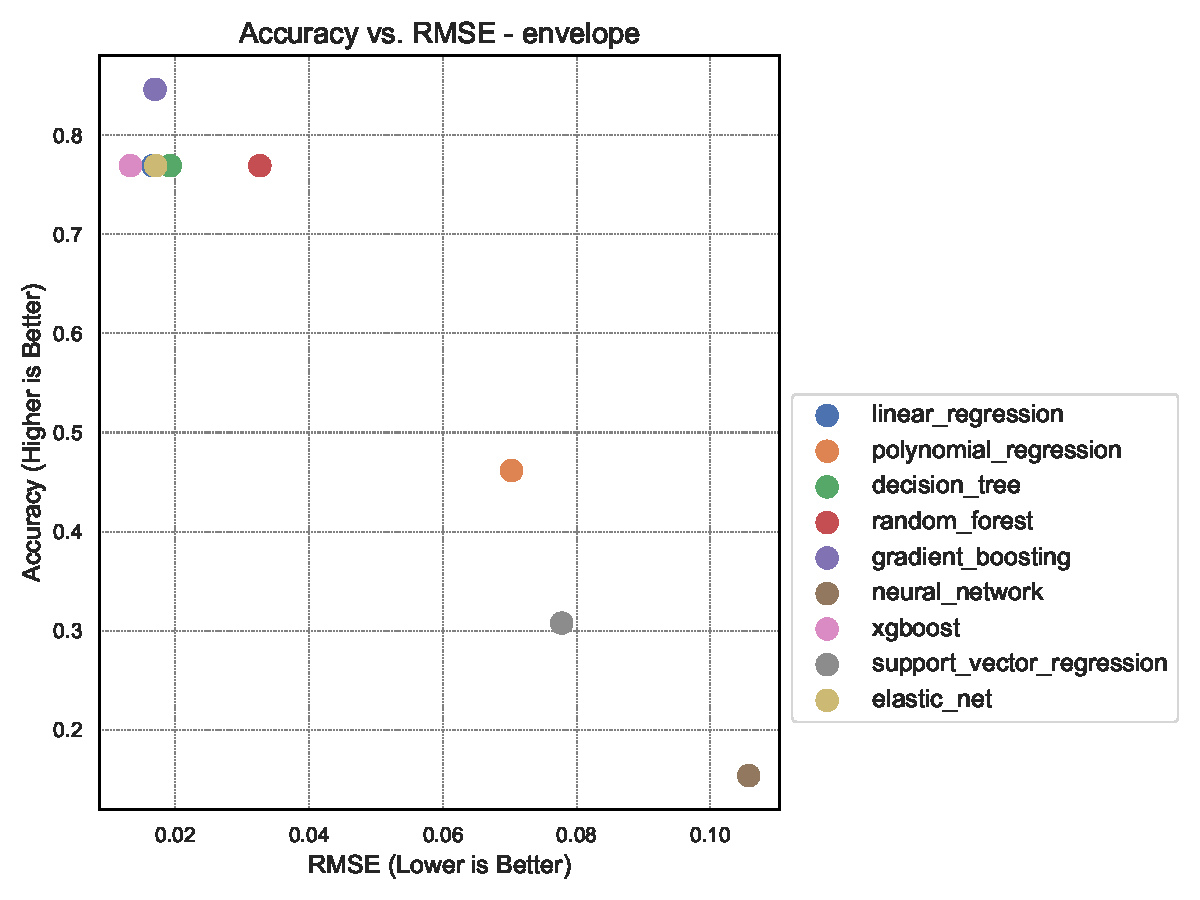
\includegraphics[width=\textwidth]{assets/images/05/accuracy_by_rmse_per_model_envelope}
        \caption{Envelope}
    \end{subfigure}
    \hfill
    \begin{subfigure}[t]{0.32\textwidth}
        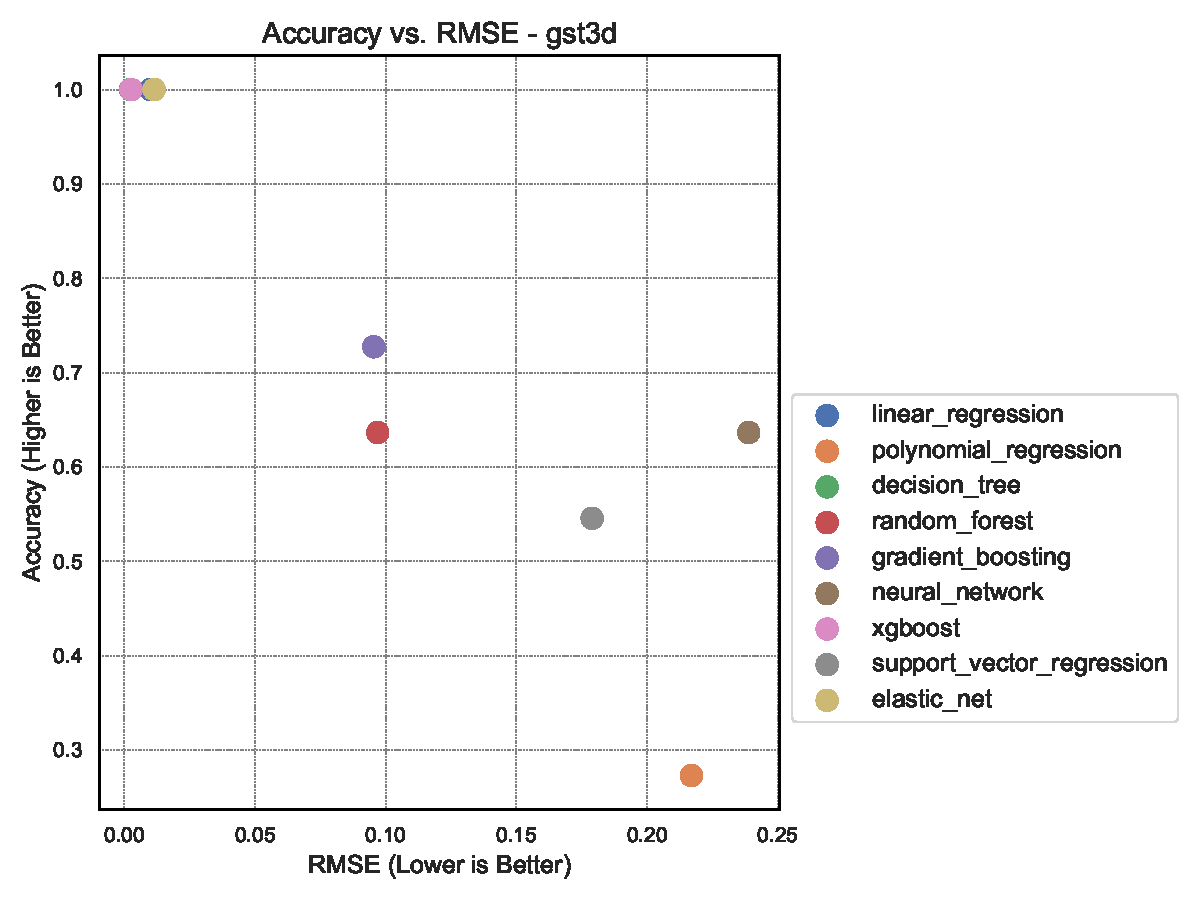
\includegraphics[width=\textwidth]{assets/images/05/accuracy_by_rmse_per_model_gst3d}
        \caption{\ac{GST3D}}
    \end{subfigure}
    \hfill
    \begin{subfigure}[t]{0.32\textwidth}
        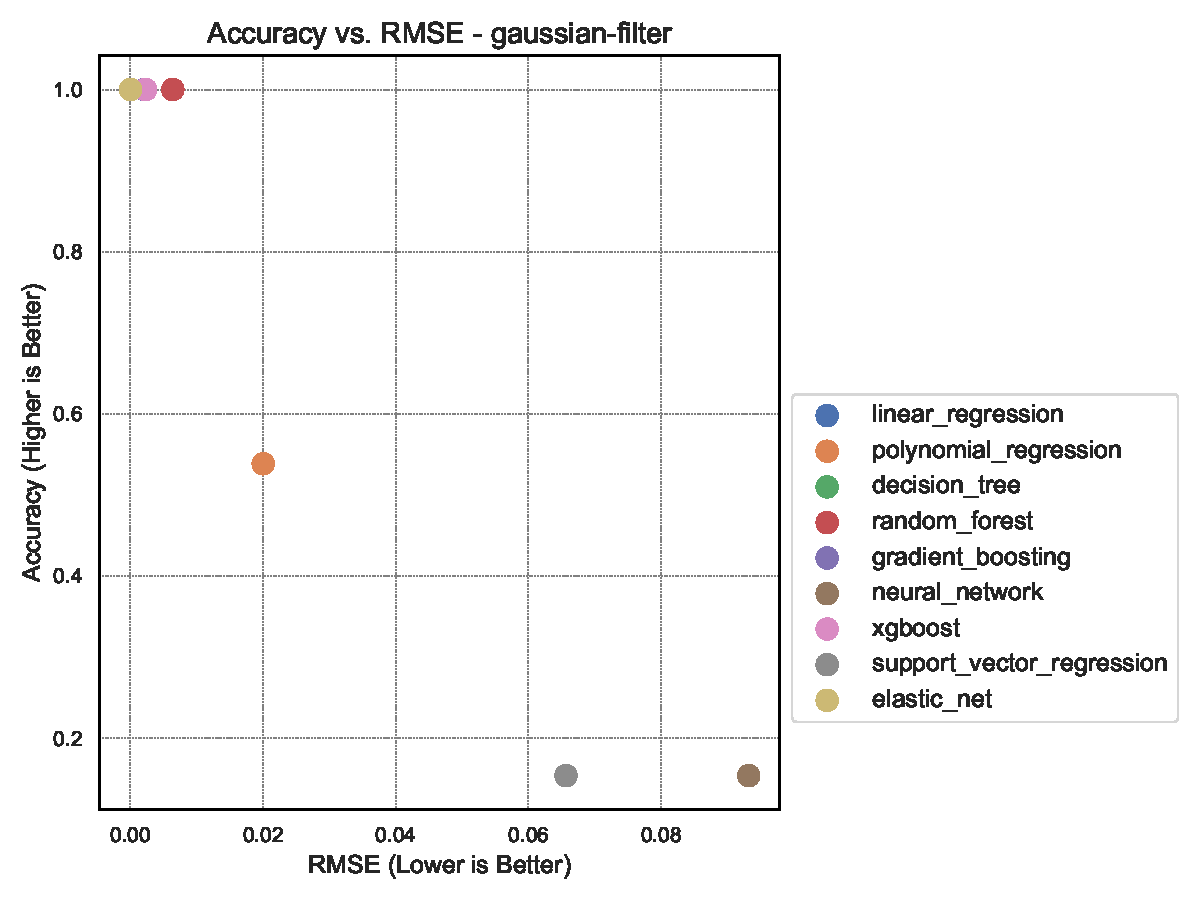
\includegraphics[width=\textwidth]{assets/images/05/accuracy_by_rmse_per_model_gaussian-filter}
        \caption{Gaussian Filter}
    \end{subfigure}
    \caption{Accuracy vs.\ \ac{RMSE} per model and operator.
        Most methods attain near-perfect metrics for Envelope and Gaussian Filter.
        \ac{GST3D} displays higher \ac{RMSE} for polynomial and Neural Network approaches.
        \EB{Acho que ficaria melhor compartilhando a legenda - com apenas uma legenda.}
    }
    \label{fig:accuracy_rmse_envelope}
\end{figure*}

\subsection{Actual vs.\ Predicted Plots and Residual Distributions}
\label{subsec:actual-vs-predicted-and-residual-distributions}

Figure~\ref{fig:actual_vs_predicted} compare actual and predicted memory usage for each operator and model.
The best fits produce data points that lie close to the diagonal line, implying minimal error.
Linear Regression, XGBoost, and Elastic Net nearly overlap with the diagonal for Envelope and Gaussian Filter.
Decision Tree does likewise for \ac{GST3D}.

\begin{figure*}[htbp]
    \centering
    \begin{subfigure}[t]{0.32\textwidth}
        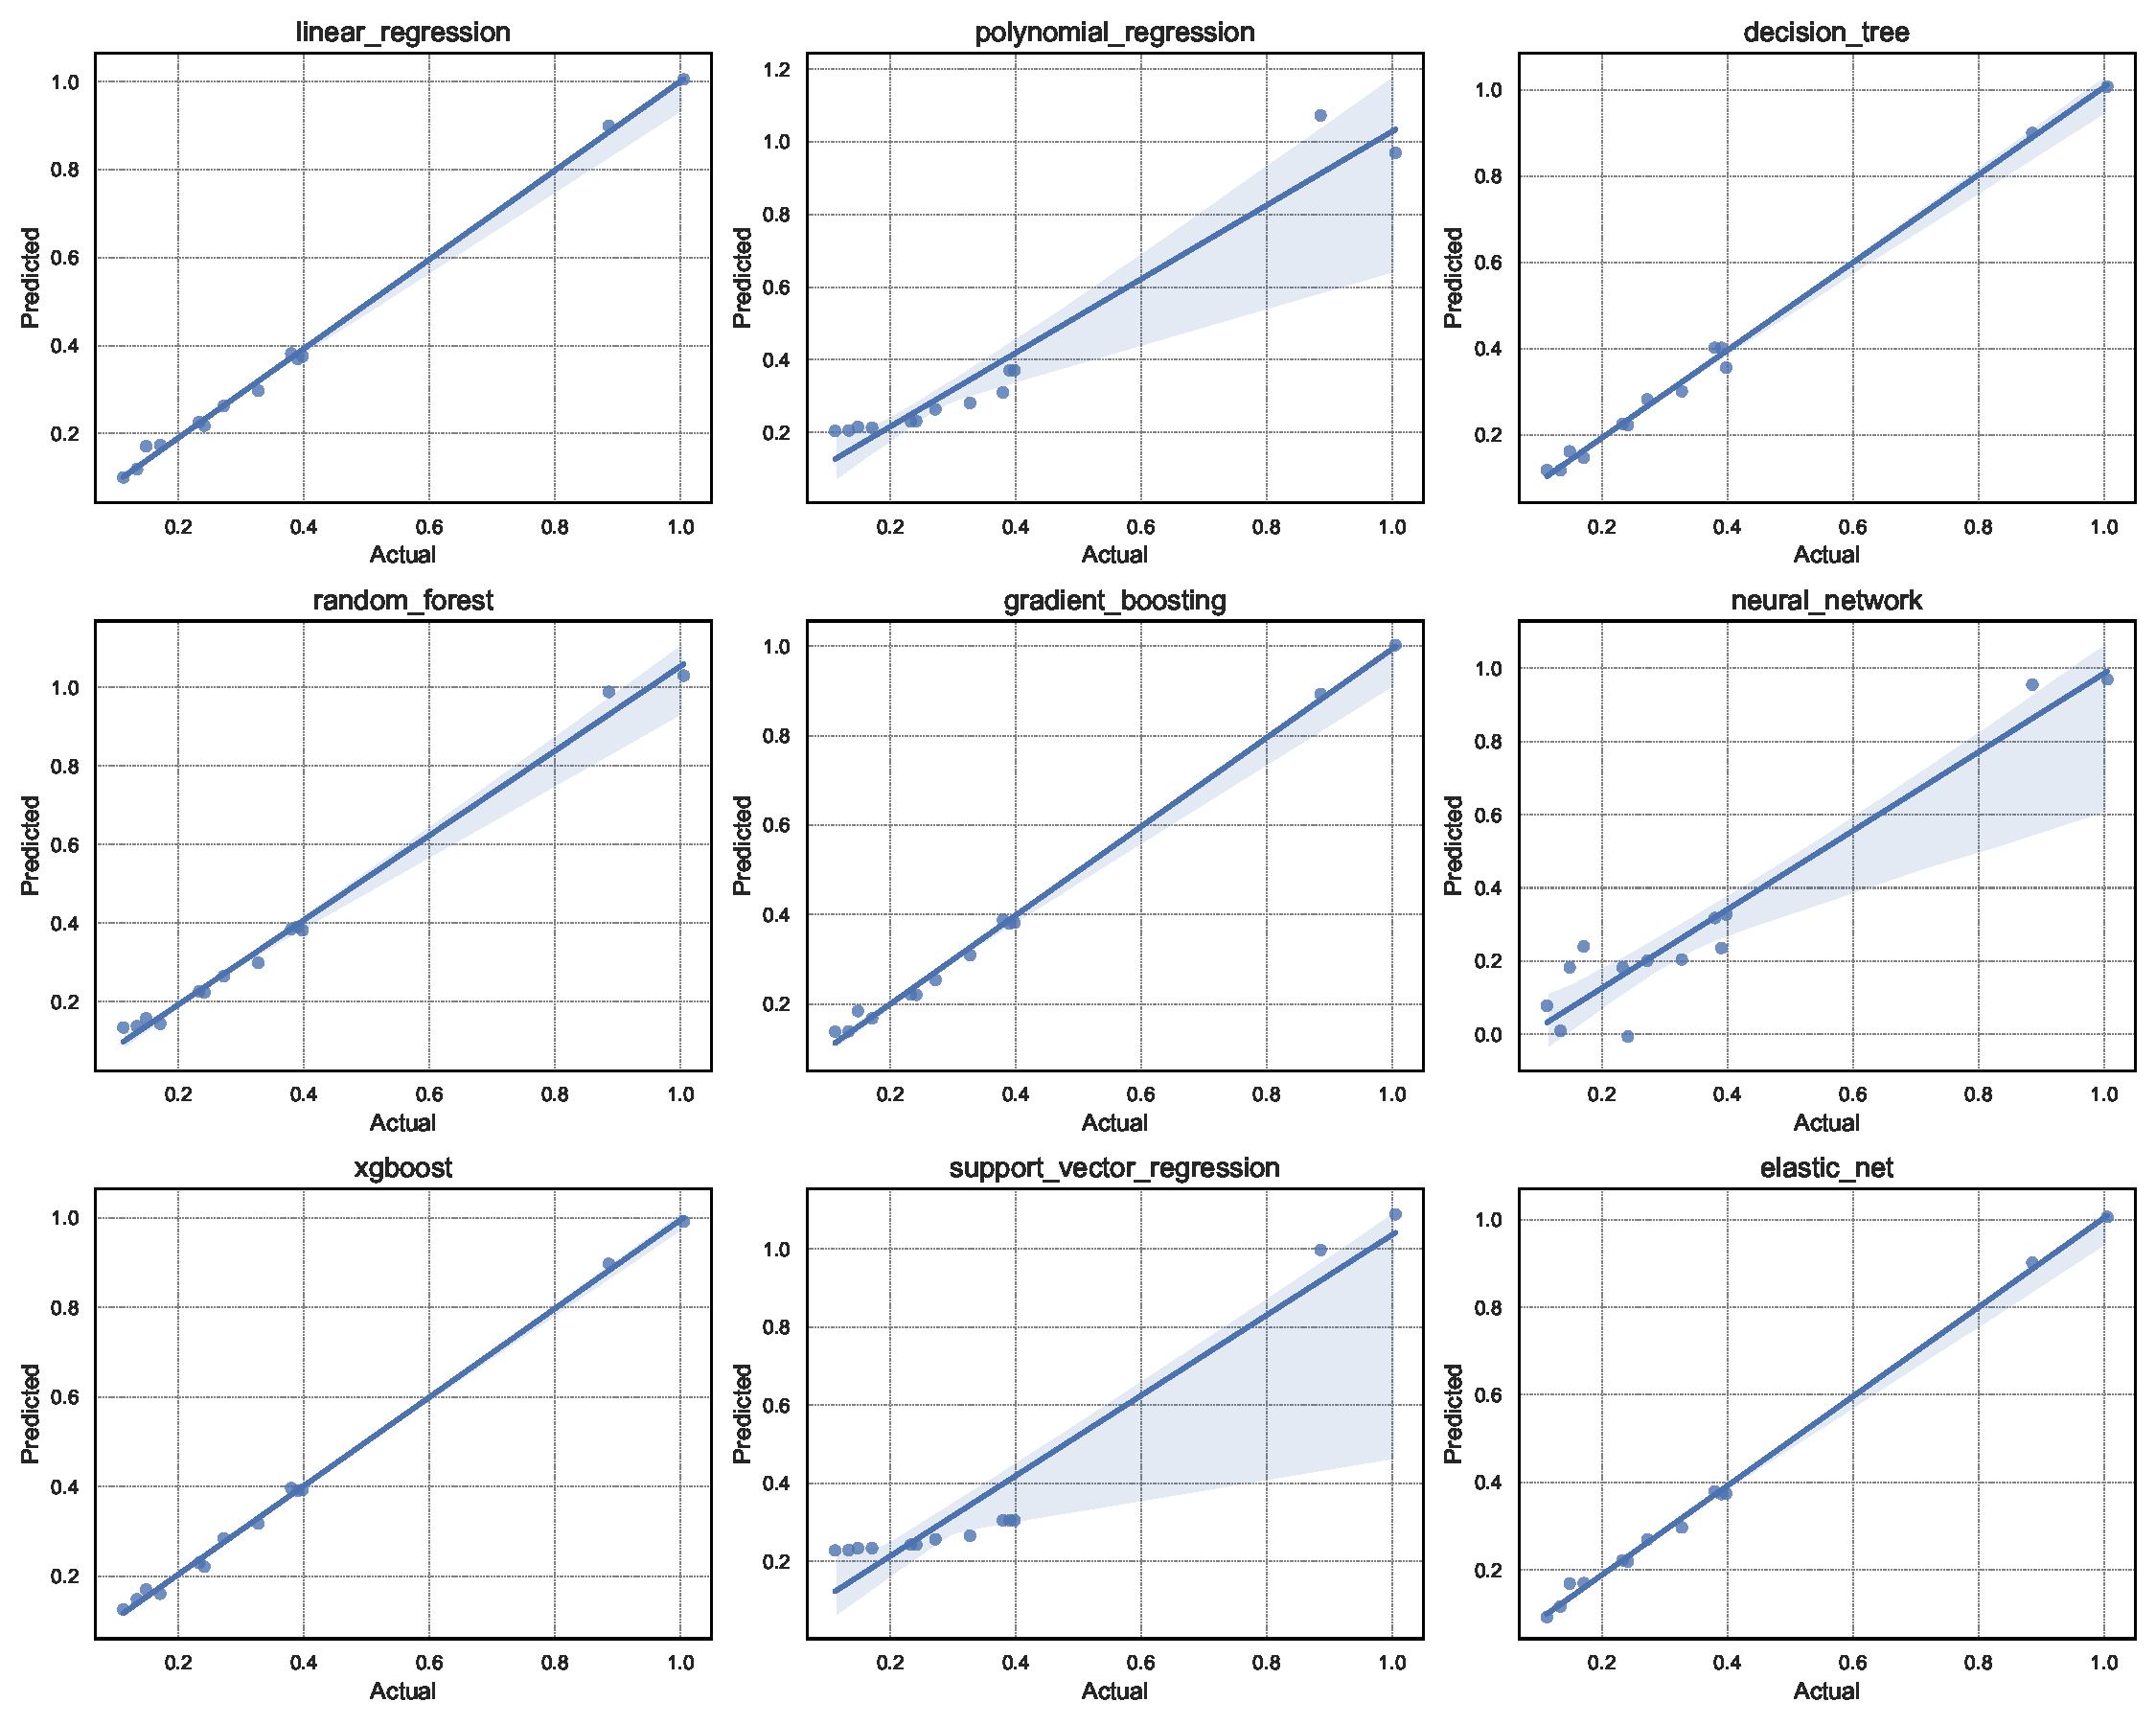
\includegraphics[width=\textwidth]{assets/images/05/actual_vs_predicted_by_model_envelope}
        \caption{Envelope}
    \end{subfigure}
    \hfill
    \begin{subfigure}[t]{0.32\textwidth}
        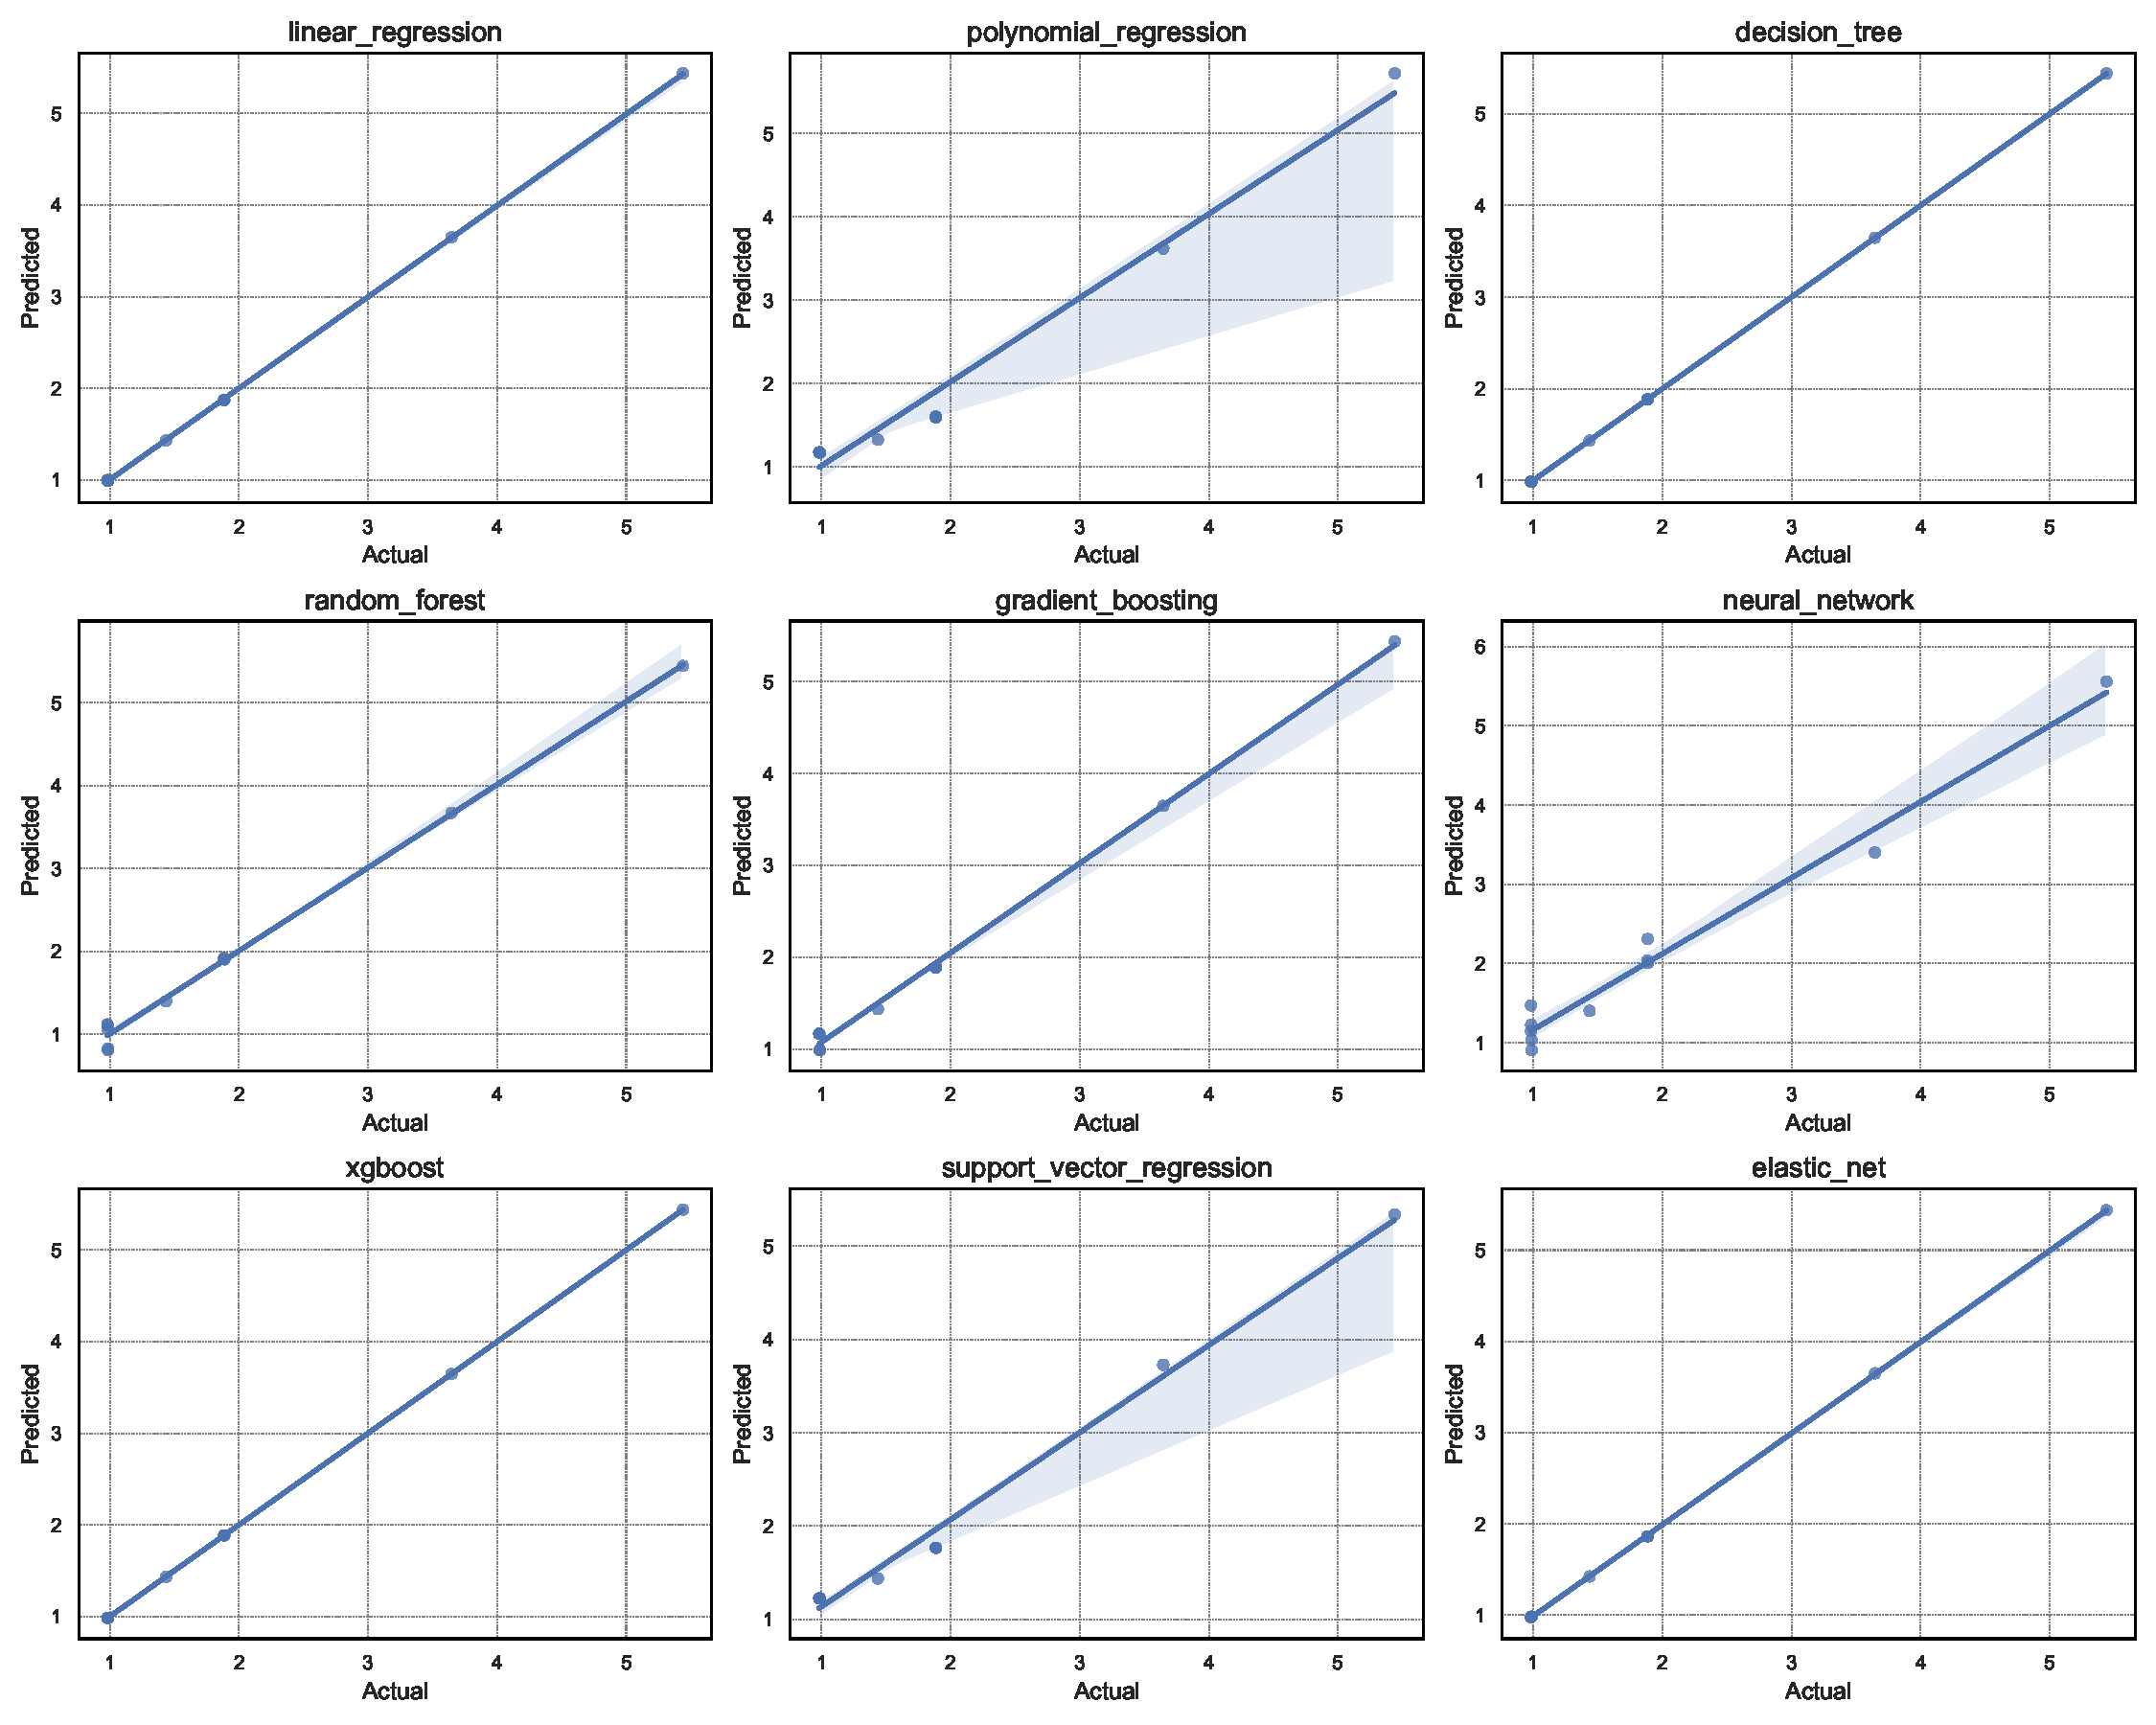
\includegraphics[width=\textwidth]{assets/images/05/actual_vs_predicted_by_model_gst3d}
        \caption{\ac{GST3D}}
    \end{subfigure}
    \hfill
    \begin{subfigure}[t]{0.32\textwidth}
        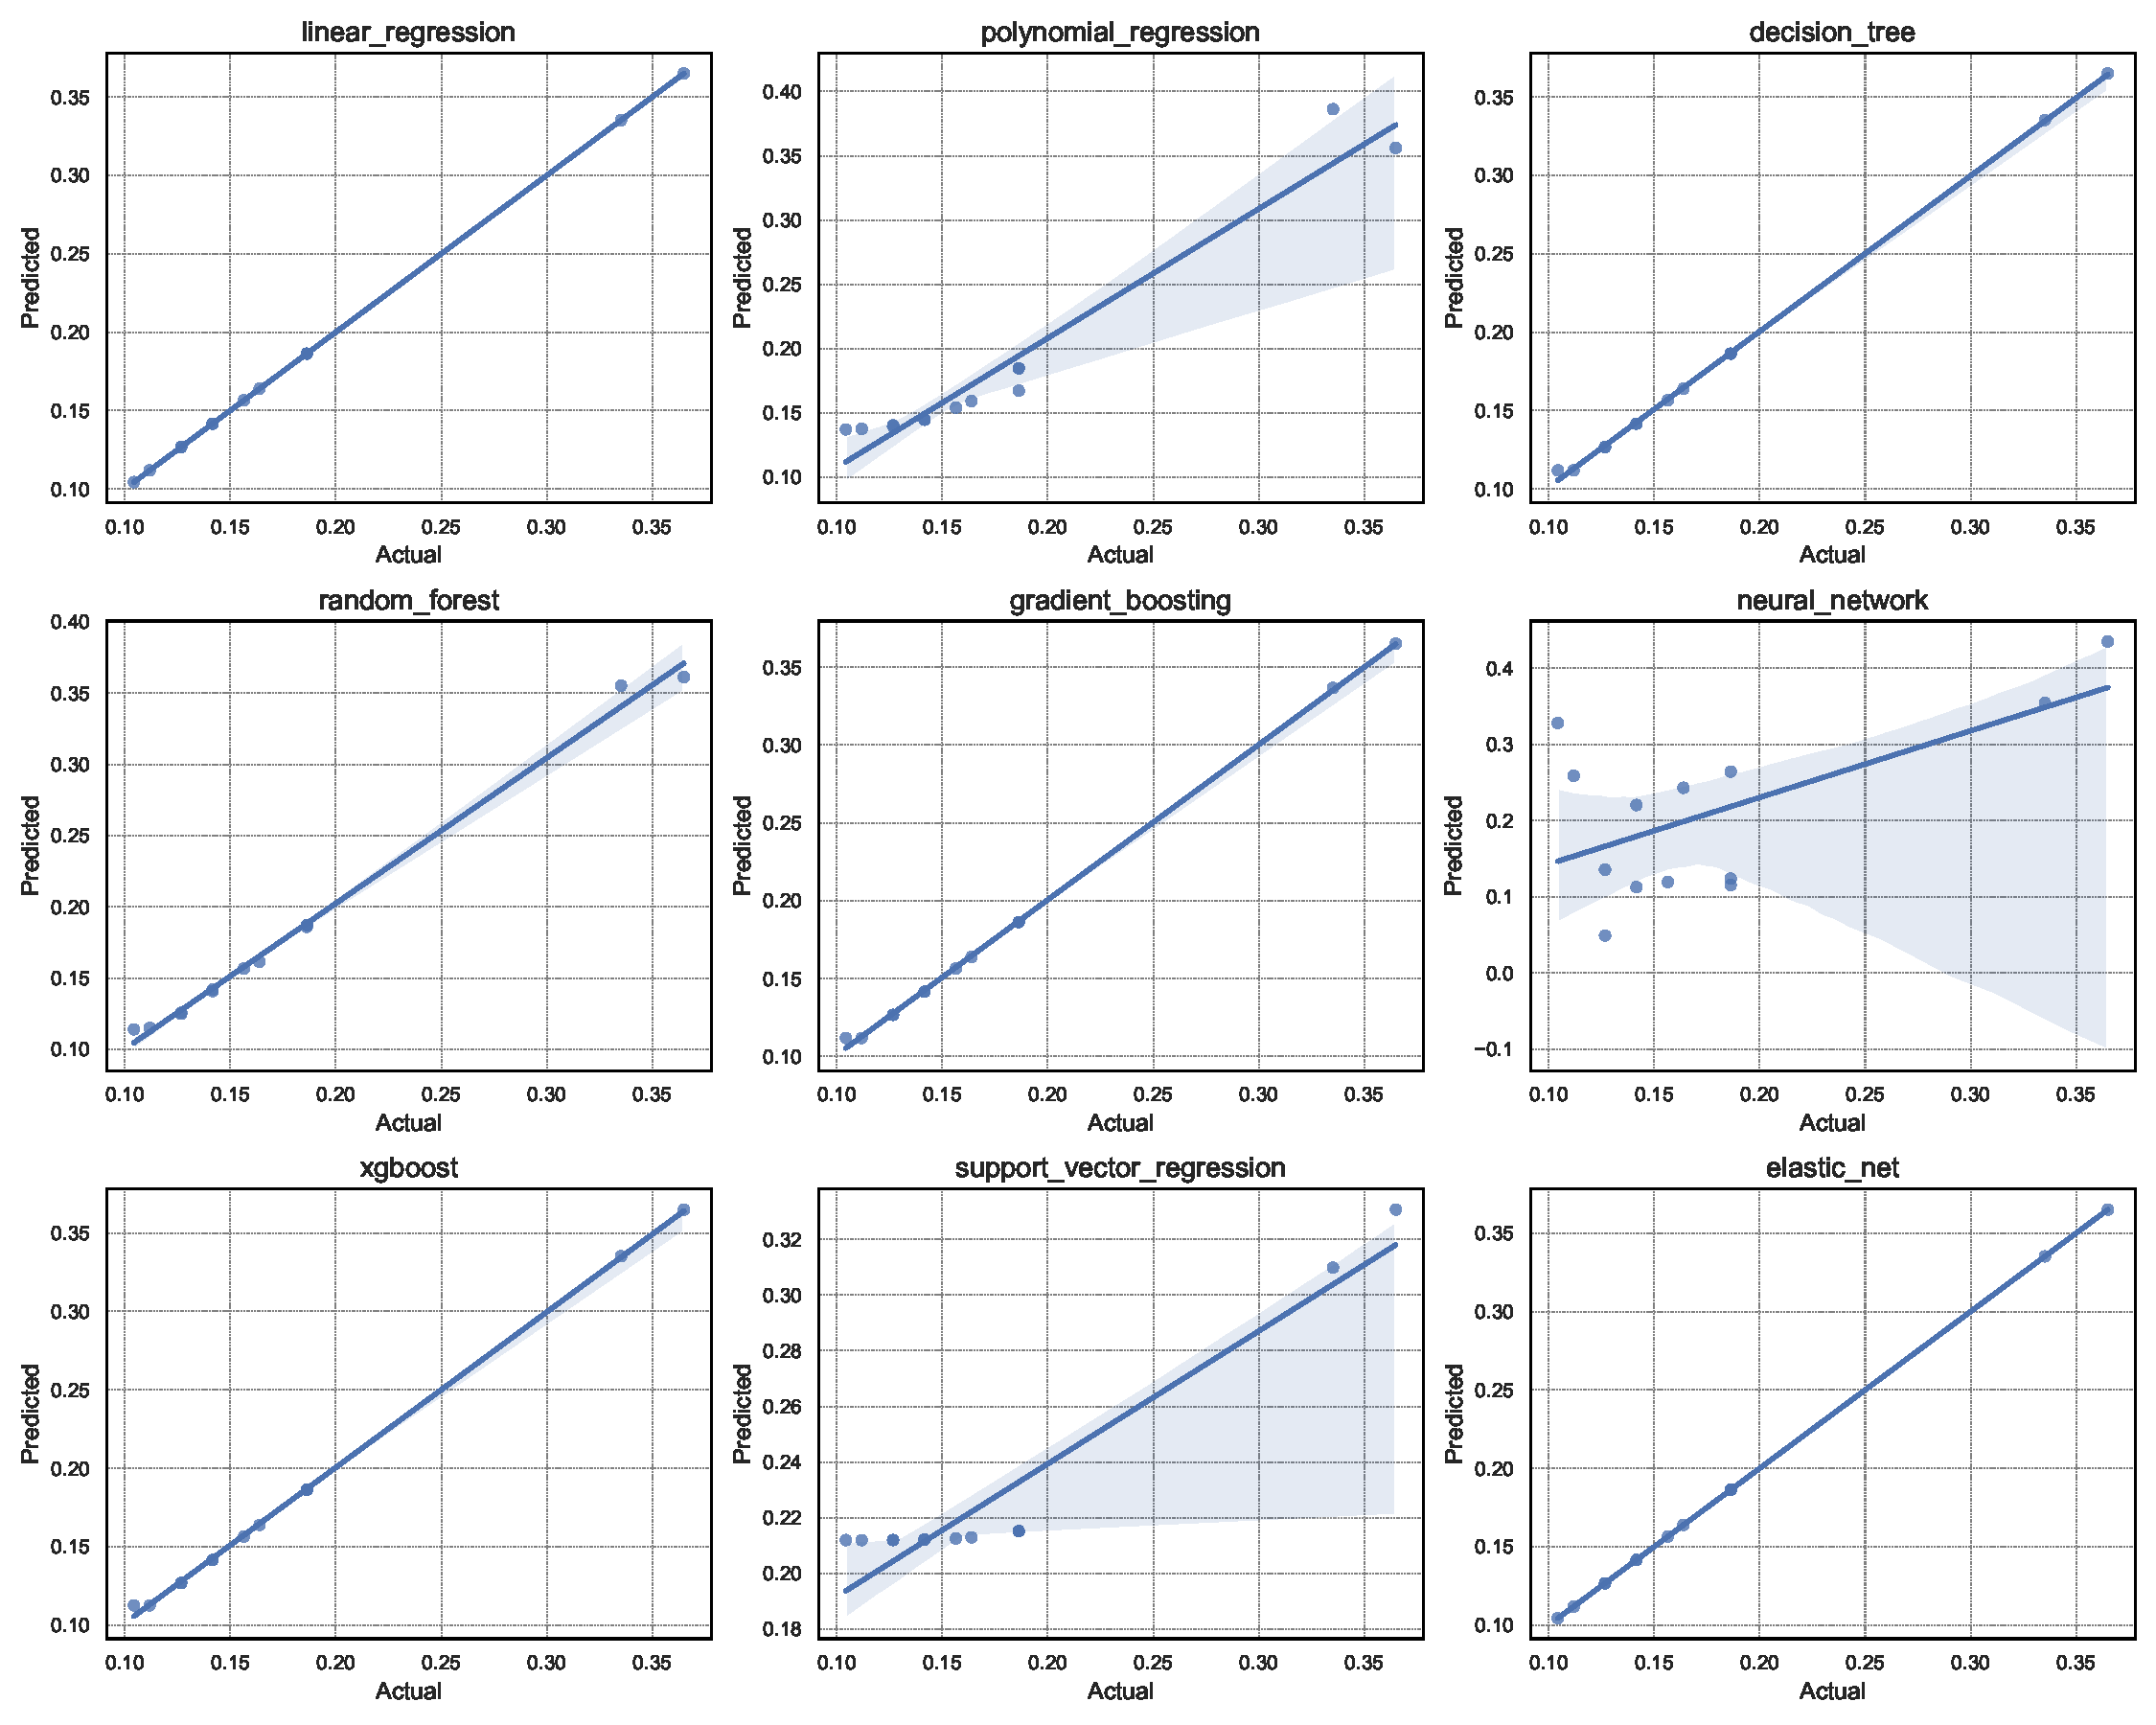
\includegraphics[width=\textwidth]{assets/images/05/actual_vs_predicted_by_model_gaussian-filter}
        \caption{Gaussian Filter}
    \end{subfigure}
    \caption{Actual vs.\ predicted memory usage for each operator.
    A nearly diagonal trend indicates that the model approximates the real consumption.
    The Neural Network struggles slightly more for \ac{GST3D}, but most others fit well.}
    \label{fig:actual_vs_predicted}
\end{figure*}

Figures~\ref{fig:residual_qq_plots} show residual \ac{QQ} plots.
Points that track the diagonal suggest normally distributed residuals, indicating no major systematic bias.
Gradient Boosting, Random Forest, and XGBoost residuals remain closer to this line than Neural Network or Polynomial Regression, which exhibit heavier tails or skew.
However, none of the models produce perfectly normal residuals, which is common in real-world \ac{HPC} \EBC{data.}{Adicionar uma referência para dar suporte a esta afirmação}

\begin{figure*}[htbp]
    \centering
    \begin{subfigure}[t]{0.32\textwidth}
        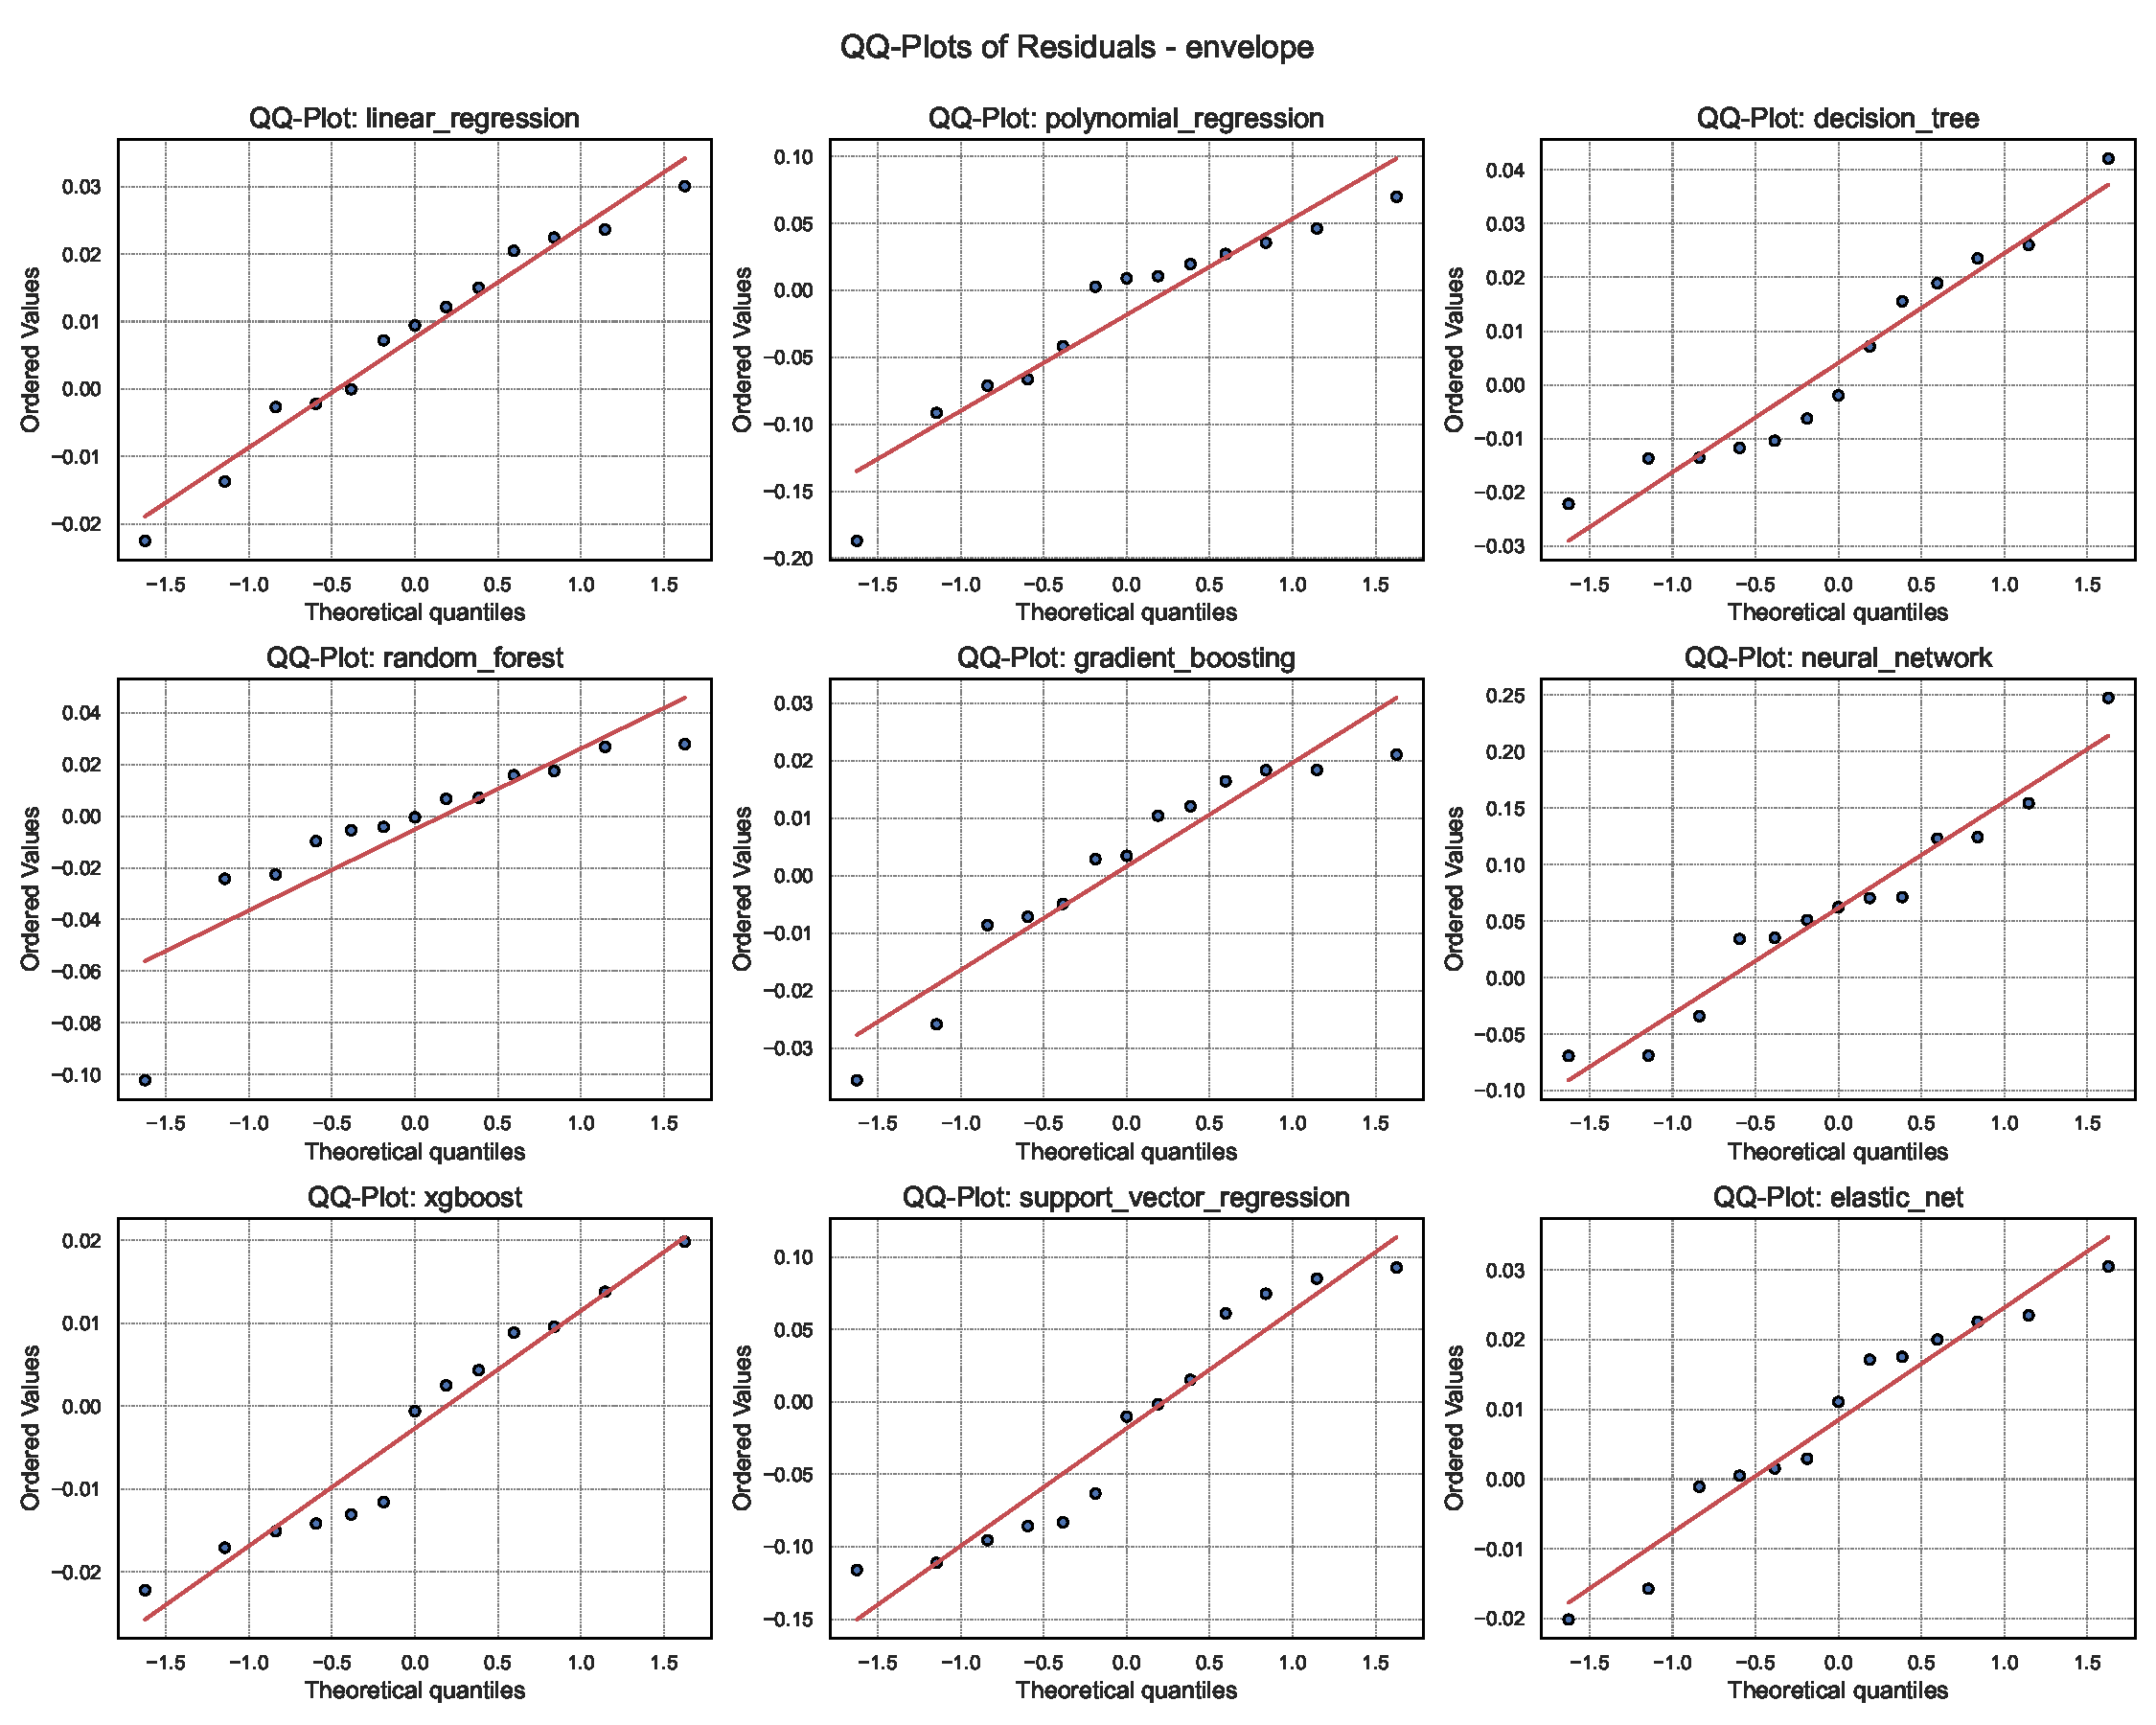
\includegraphics[width=\textwidth]{assets/images/05/residual_qq_plots_envelope}
        \caption{Envelope}
    \end{subfigure}
    \hfill
    \begin{subfigure}[t]{0.32\textwidth}
        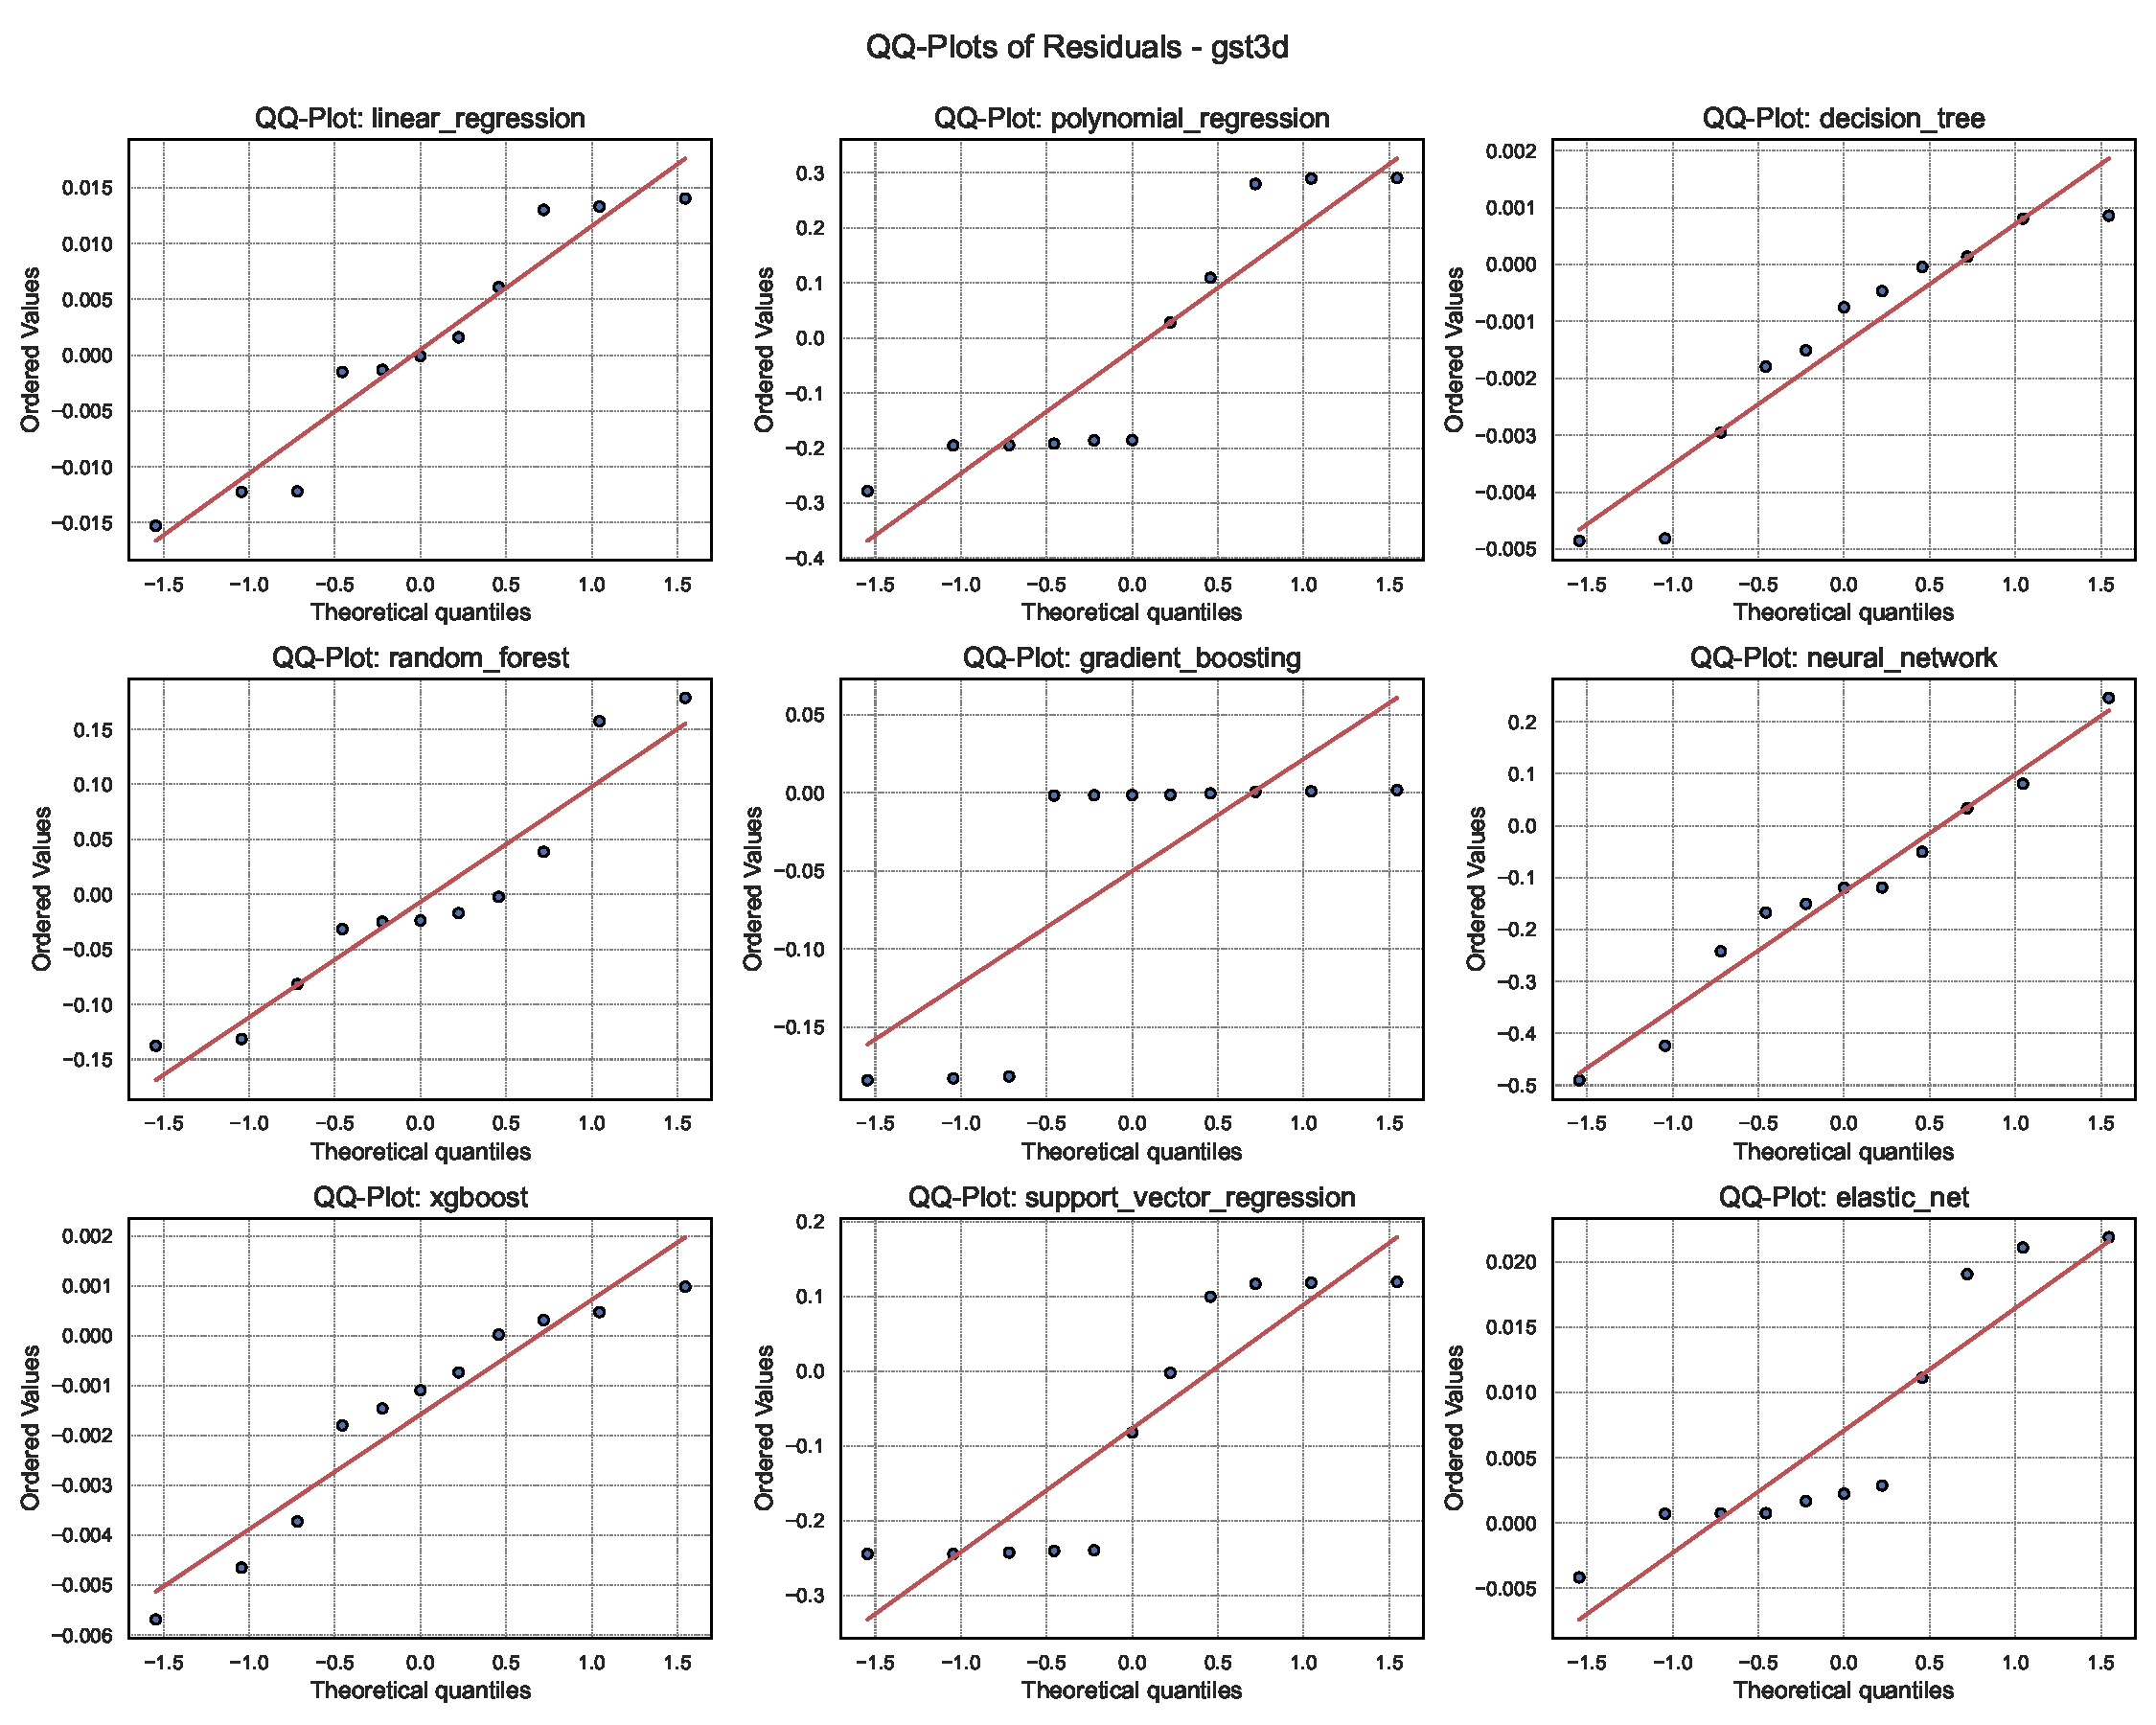
\includegraphics[width=\textwidth]{assets/images/05/residual_qq_plots_gst3d}
        \caption{\ac{GST3D}}
    \end{subfigure}
    \hfill
    \begin{subfigure}[t]{0.32\textwidth}
        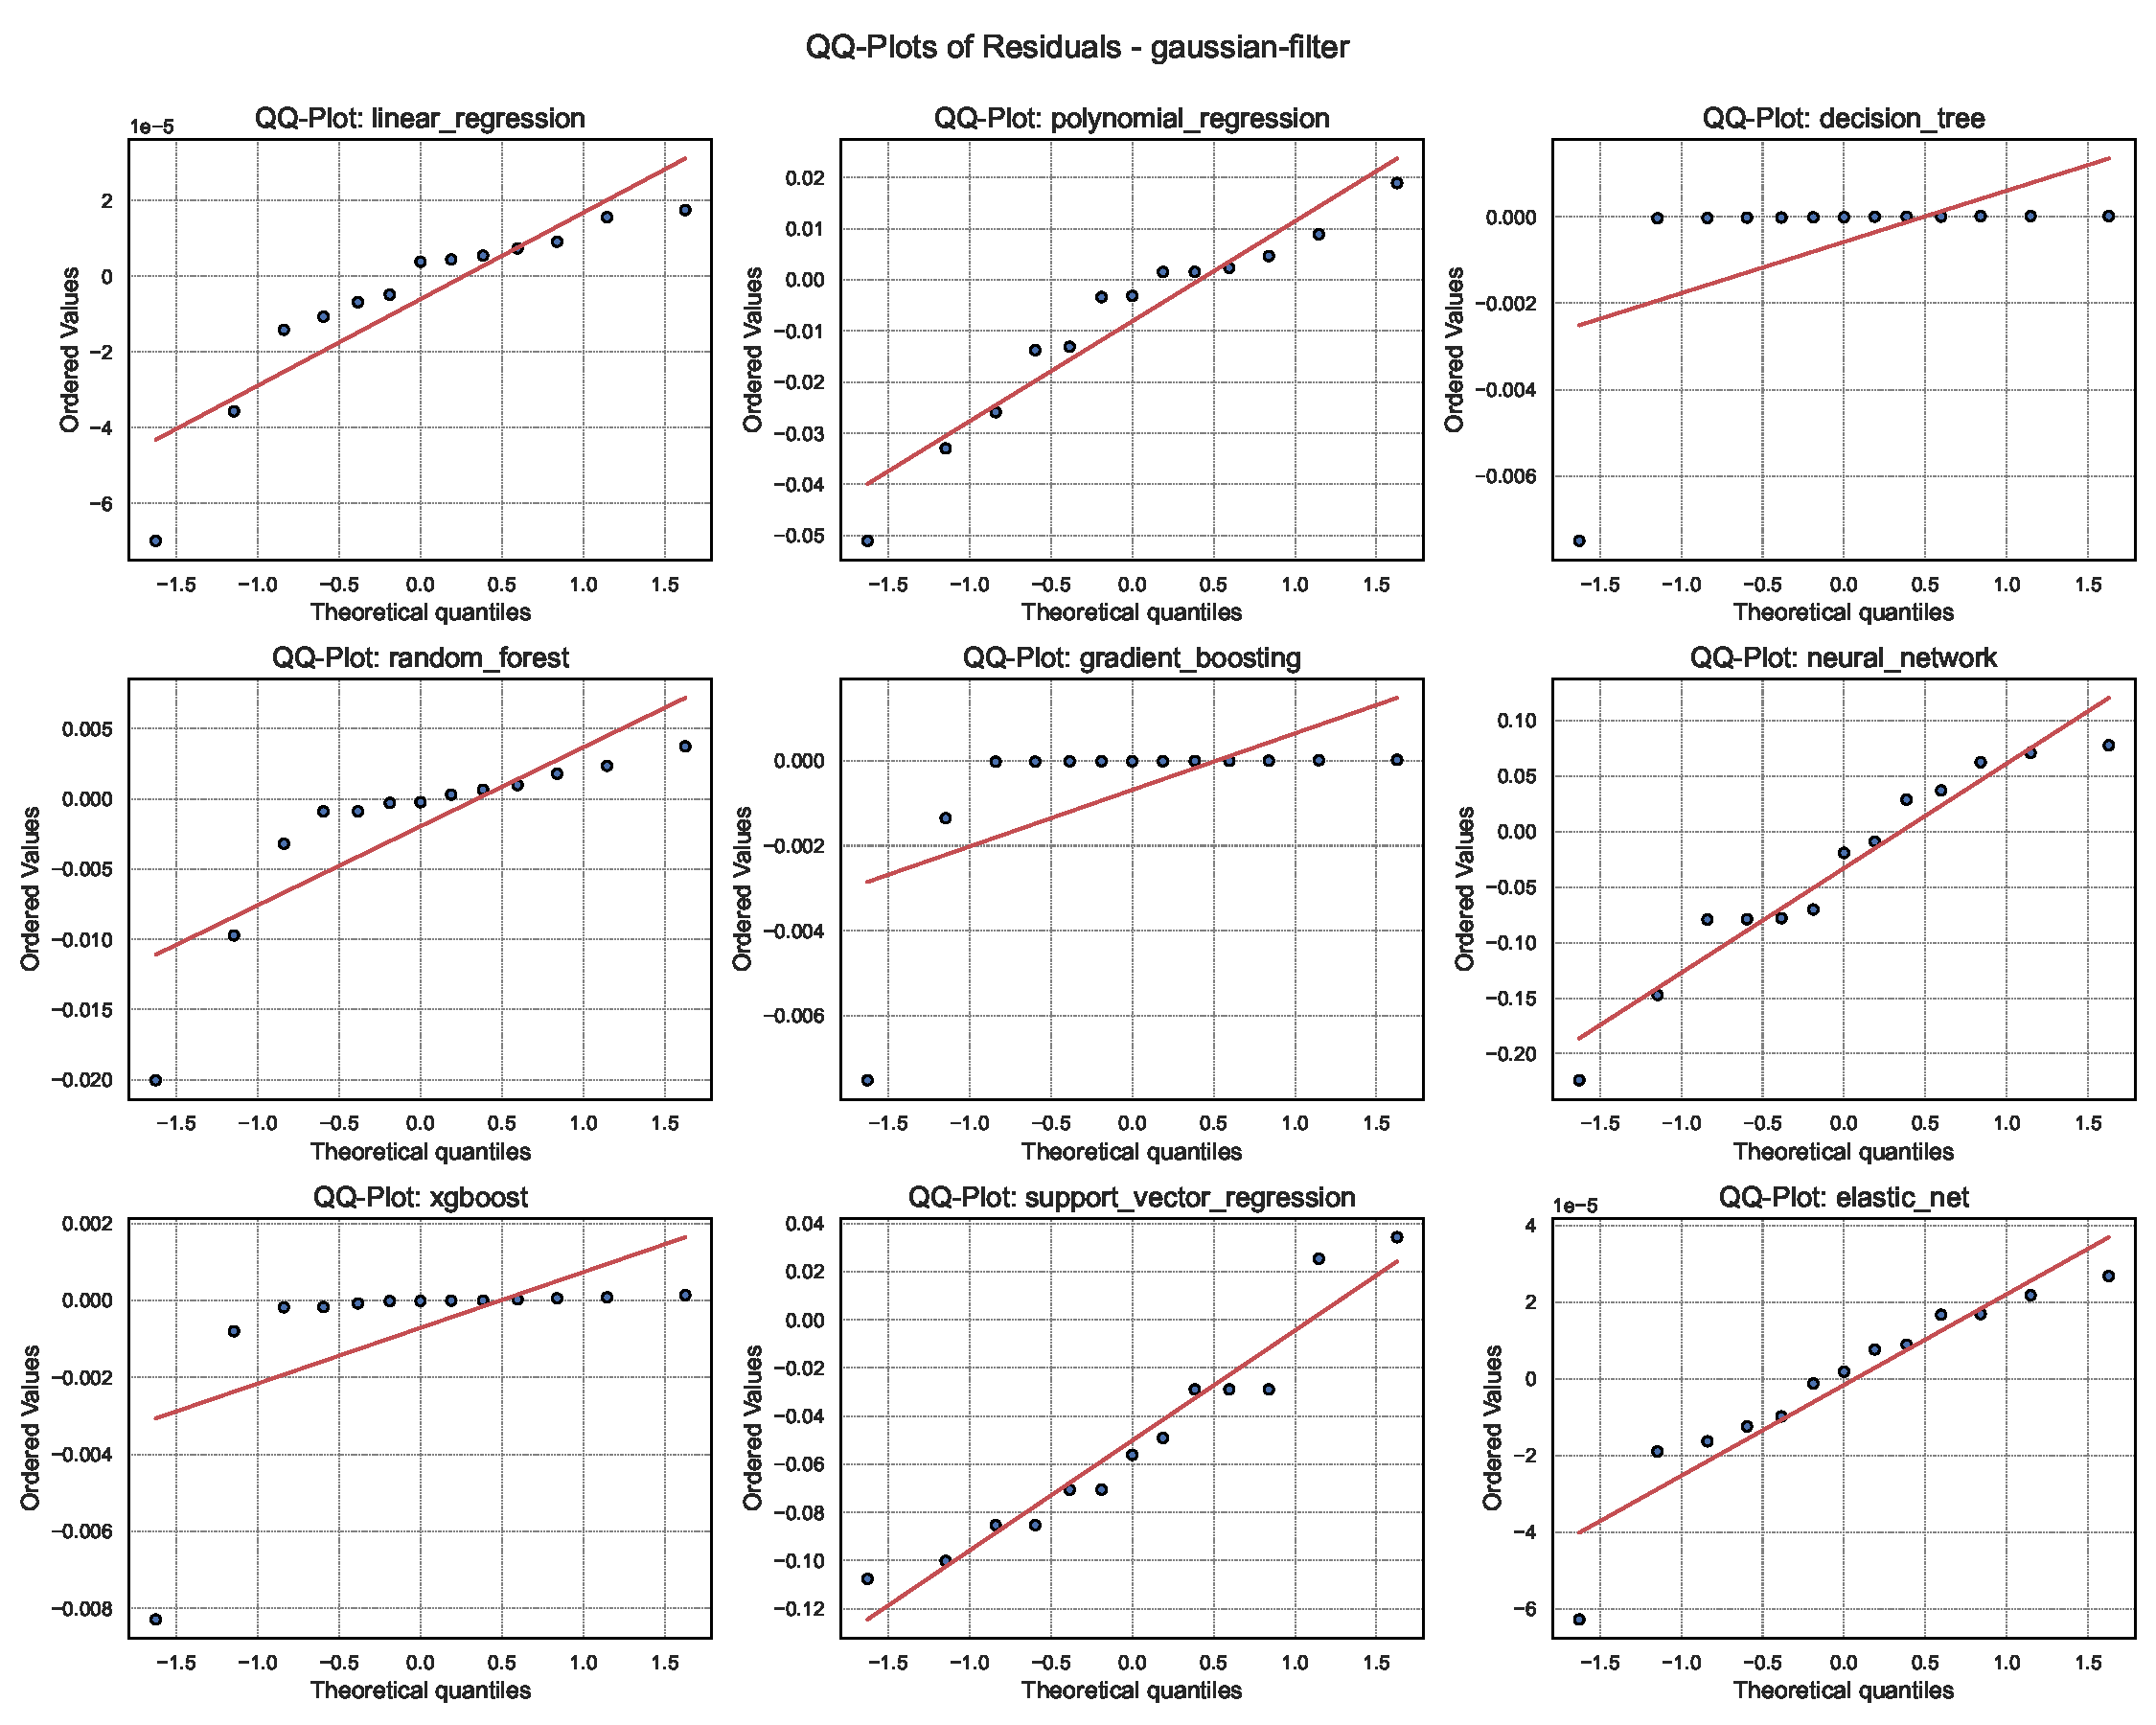
\includegraphics[width=\textwidth]{assets/images/05/residual_qq_plots_gaussian-filter}
        \caption{Gaussian Filter}
    \end{subfigure}
    \caption{\ac{QQ} plots of model residuals by operator.
        Most methods exhibit mild deviations from normality in the tails.
        Neural Network displays noticeably heavier upper-tail errors for \ac{GST3D}.
        \EB{Os rótulos ficaram muito pequenos. Será que este gráfico é necessário?}
        \label{fig:residual_qq_plots}
    }
\end{figure*}

\subsection{Performance Summary}
\label{subsec:performance-summary}

Figures~\ref{fig:performance_by_model_operators} compile \ac{RMSE}, \ac{MAE}, $R^2$, and accuracy into a single bar chart for each operator, offering a side-by-side visualization of model performance.
All charts reinforce the earlier observation that memory usage for Envelope and Gaussian Filter proves easier to capture accurately than \ac{GST3D}.
Decision Tree, Gradient Boosting, and XGBoost often yield high precision for \ac{GST3D}, whereas Neural Network and Polynomial Regression struggle with larger errors.

\begin{figure*}[htbp]
    \centering
    \begin{subfigure}[t]{0.32\textwidth}
        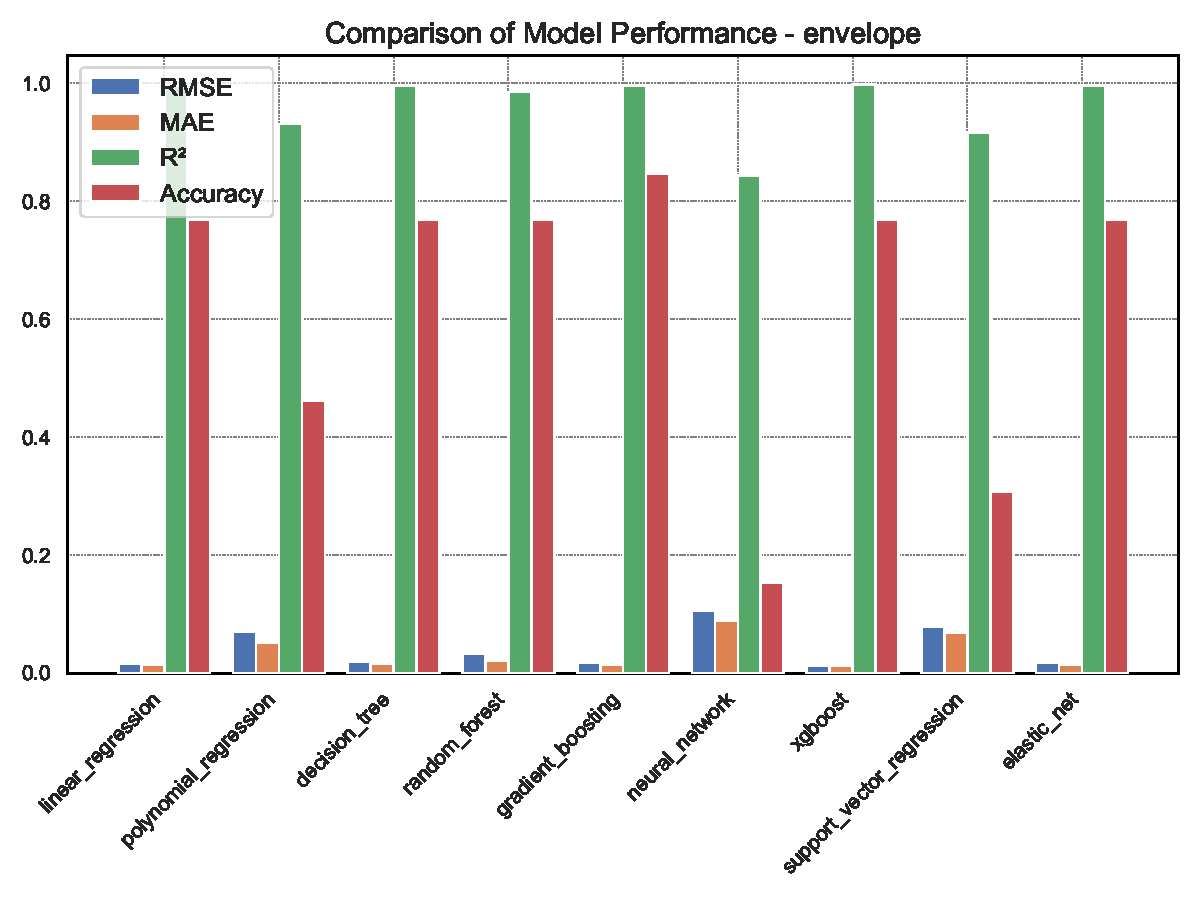
\includegraphics[width=\textwidth]{assets/images/05/performance_by_model_envelope}
        \caption{Envelope}
    \end{subfigure}
    \hfill
    \begin{subfigure}[t]{0.32\textwidth}
        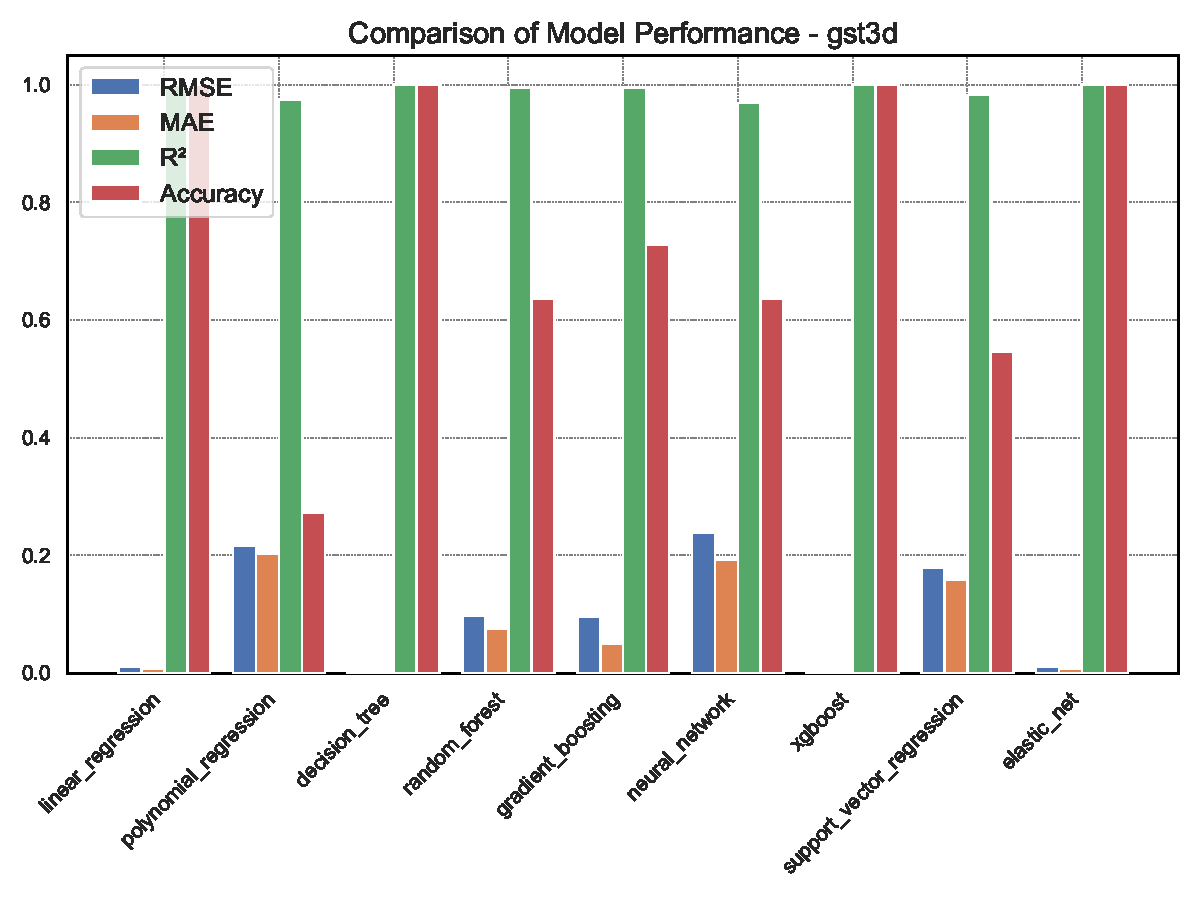
\includegraphics[width=\textwidth]{assets/images/05/performance_by_model_gst3d}
        \caption{\ac{GST3D}}
    \end{subfigure}
    \hfill
    \begin{subfigure}[t]{0.32\textwidth}
        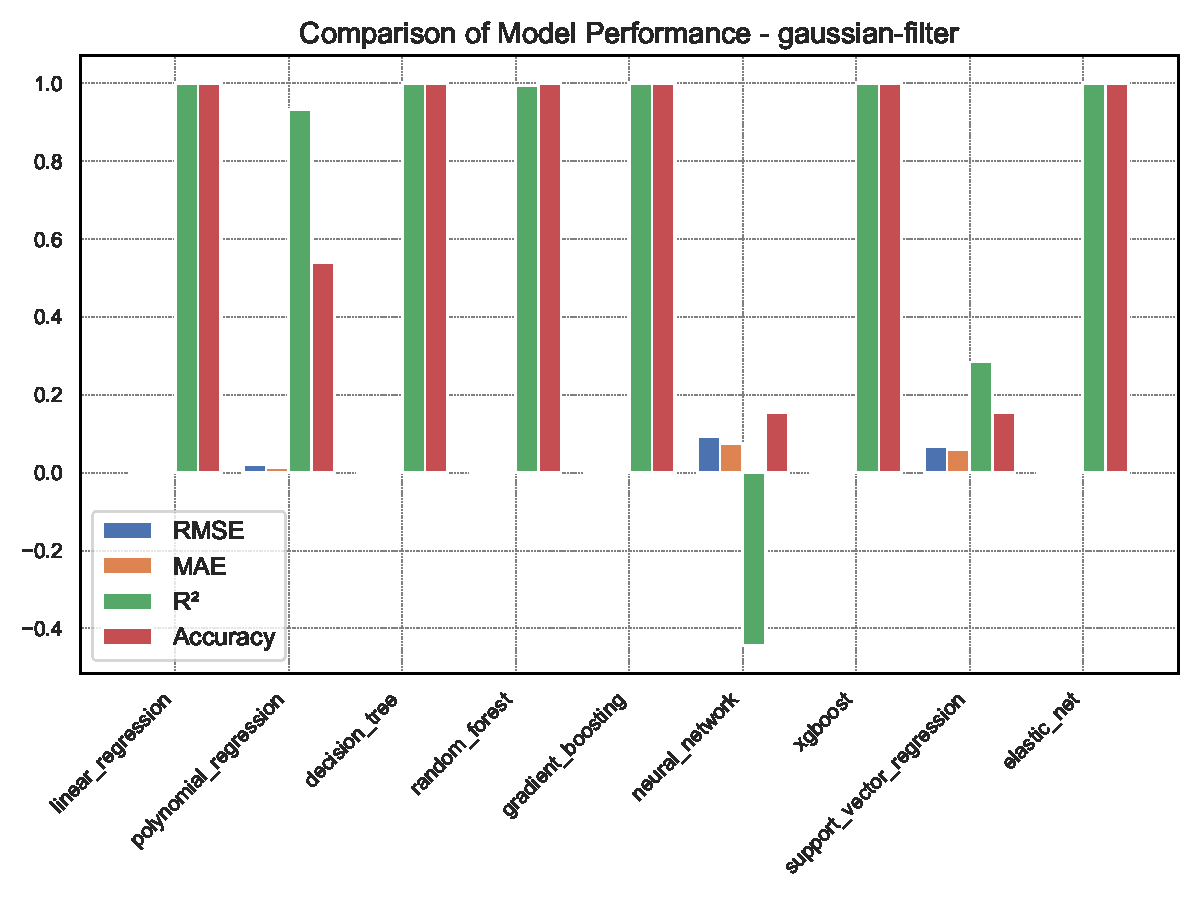
\includegraphics[width=\textwidth]{assets/images/05/performance_by_model_gaussian-filter}
        \caption{Gaussian Filter}
    \end{subfigure}
    \caption{Model metrics (\ac{RMSE}, \ac{MAE}, $R^2$, and accuracy) by operator.
        Best-in-class methods include Gradient Boosting (Envelope), Decision Tree (\ac{GST3D}), and Linear Regression (Gaussian Filter).
        \EB{Daniel, uma avaliação com valores RMSE e MAE deve levar em consideração o valor da predição - p.ex., um erro (RMSE ou MAE) de 0.1GB é pequeno em uma situação onde o valor real/predito é da ordem de dezenas ou centenas de GBs, no entanto, se o valor real/predito é da ordem de 0.1GB, o erro é bem grande.}
        \label{fig:performance_by_model_operators}
    }
\end{figure*}

In summary, the near-linear dependence of peak memory on shape parameters enables multiple models to achieve excellent accuracy and reliability.
Envelope and Gaussian Filter place fewer demands on model complexity.
\ac{GST3D} remains more challenging, though tree-based models and linear approaches still achieve high $R^2$ and low error metrics.
Neural Network stands out for relatively weaker performance in \ac{GST3D}, suggesting that the chosen architecture or hyperparameters might require further tuning for more complex operators.

All subsequent sections build on these findings to evaluate feature selection (Section~\ref{sec:pmc-results-feature-selection-experiments}) and data size reductions (Section~\ref{sec:pmc-results-data-reduction-studies}), aiming to determine whether simpler input representations or smaller datasets can maintain the strong predictive performance observed in these experiments.
\section{Feature Selection Experiments}
\label{sec:pmc-results-feature-selection-experiments}

\EB{Daniel, me parece que seria mais natural apresentar o processo de seleção de features antes das seções que realizam a análise dos dados já pressupondo o uso da feature volume.}

This section investigates the impact of eliminating various shape-derived features on model accuracy, with a particular focus on verifying whether \emph{volume} alone is \EBC{sufficient to predict peak memory usage}{Você já mostrou que a feature volume tem uma relação bem simples (linear) com o pico de consumo de memória.}.
Section~\ref{sec:pmc-results-model-performance-overview} identified Gradient Boosting, Linear Regression, and Decision Tree as the best performers for Envelope, Gaussian Filter, and \ac{GST3D}, respectively.
Consequently, the experiments below use these three models when removing features.

\subsection{Volume-Centric Hypothesis}
\label{subsec:feature-selection-volume-centric-hypothesis}

Figure~\ref{fig:memory_vs_volume_regression_subplots} shows how tightly memory usage correlates with volume for Envelope, Gaussian Filter, and \ac{GST3D}.
Each subplot includes a regression fit, highlighting that volume on its own explains most of the variance.
This observation motivates a systematic “feature pruning” study to confirm whether additional descriptors (e.g., diagonal length, surface area, ratio features) offer meaningful improvements.

\begin{figure*}[htbp]
    \centering
    \begin{subfigure}[t]{0.32\textwidth}
        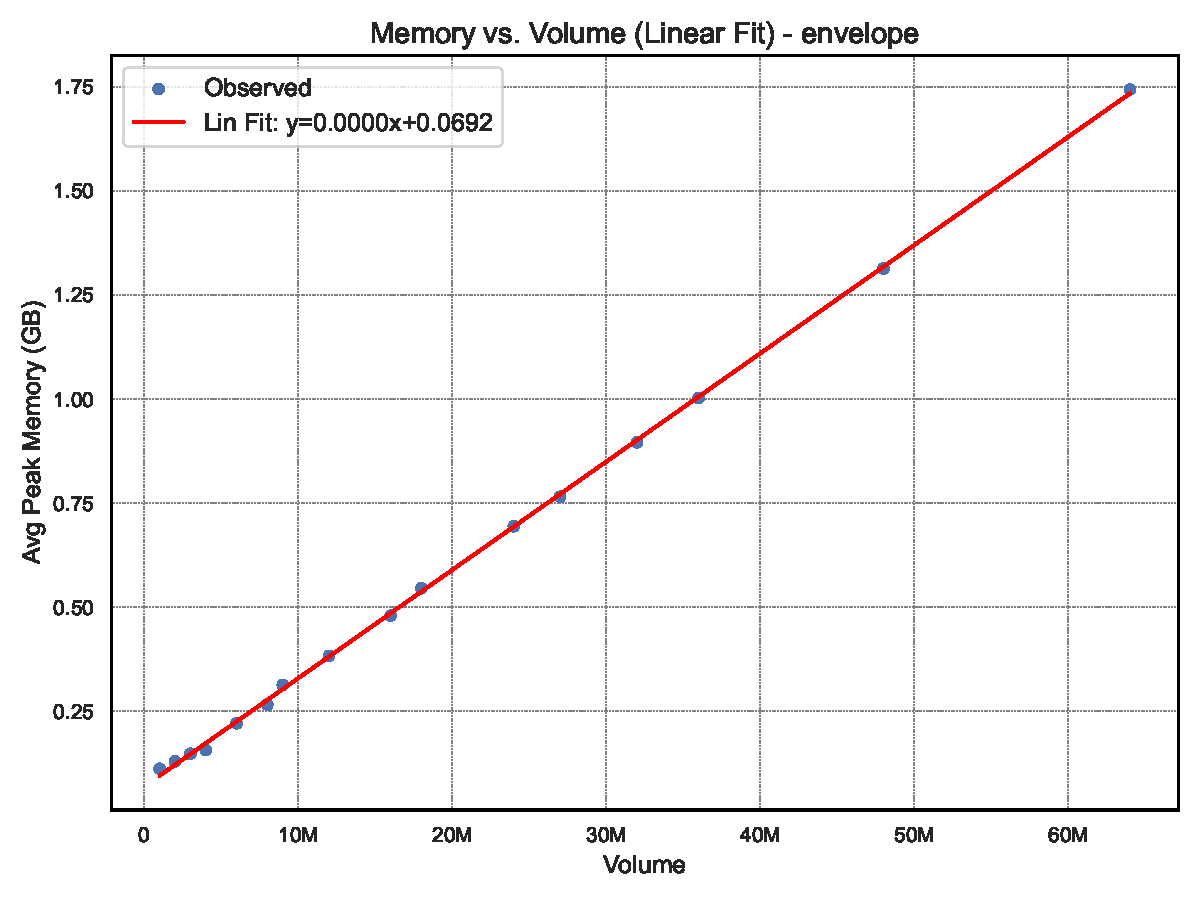
\includegraphics[width=\textwidth]{assets/images/05/memory_vs_volume_regression_envelope}
        \caption{Envelope}
    \end{subfigure}
    \hfill
    \begin{subfigure}[t]{0.32\textwidth}
        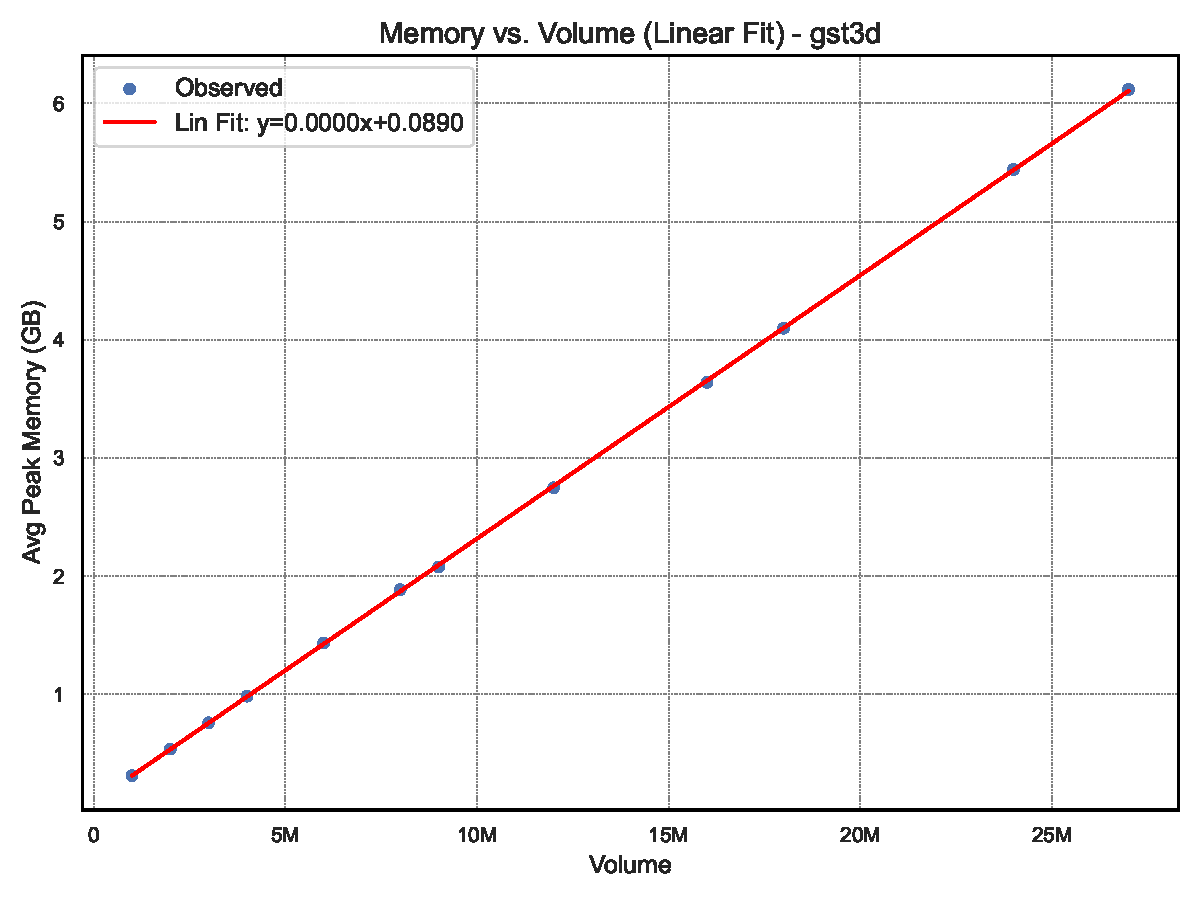
\includegraphics[width=\textwidth]{assets/images/05/memory_vs_volume_regression_gst3d}
        \caption{\ac{GST3D}}
    \end{subfigure}
    \hfill
    \begin{subfigure}[t]{0.32\textwidth}
        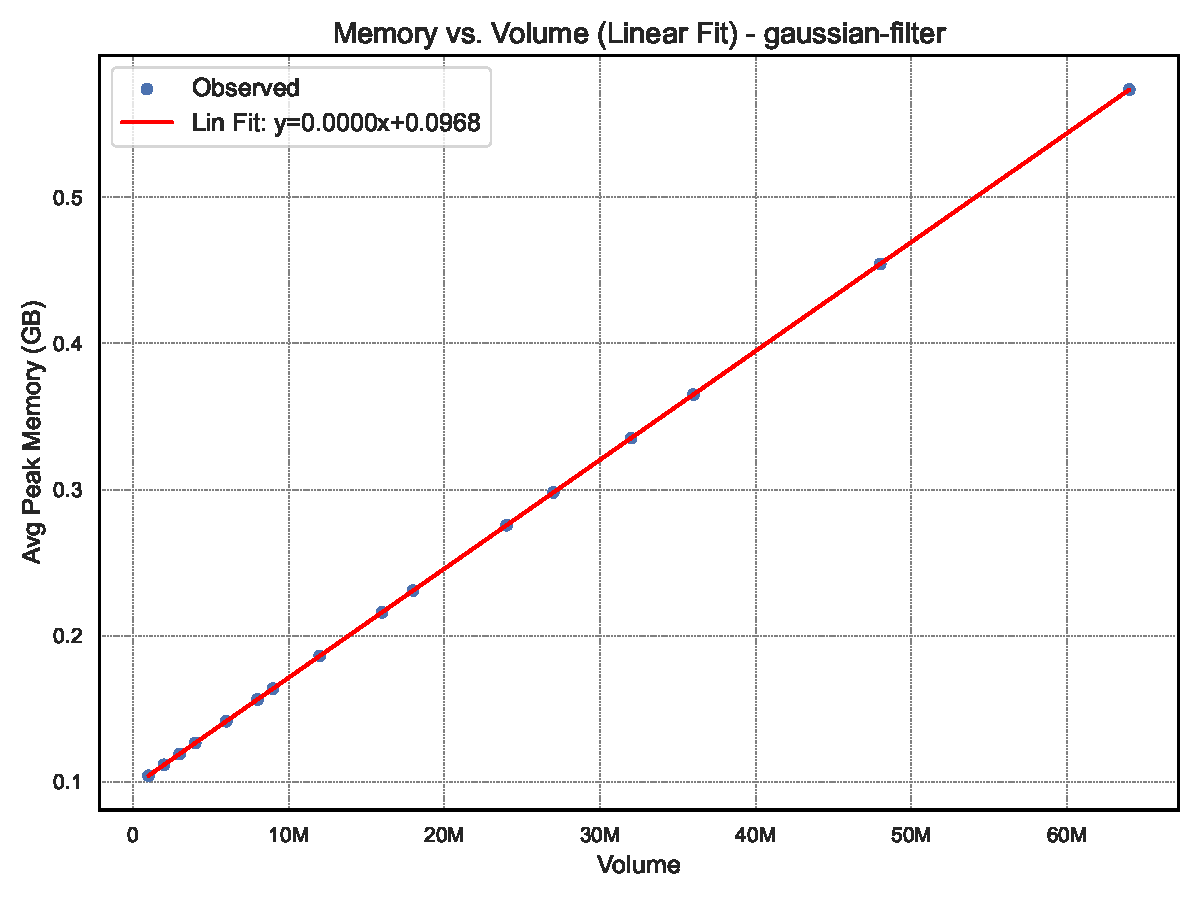
\includegraphics[width=\textwidth]{assets/images/05/memory_vs_volume_regression_gaussian-filter}
        \caption{Gaussian Filter}
    \end{subfigure}
    \caption{Memory usage vs.\ volume with regression lines for Envelope, \ac{GST3D}, and Gaussian Filter.
    All three curves reinforce that volume alone has substantial explanatory power.}
    \label{fig:memory_vs_volume_regression_subplots}
\end{figure*}

\subsection{Feature Removal Process and Metrics}
\label{subsec:feature-removal-methods-and-metrics}

The experiments adopted a stepwise strategy:
\begin{enumerate}
    \item Collect a ranked list of features using a relevance metric (e.g., \emph{SelectKBest}). \EB{Senti falta de uma explicação e/ou referências para o método SelectKBest e uma breve discussão sobre como você aplicou ele - aplicou múltiplas vezes, uma para cada modelo? Uma para cada operador? uma única vez e gerou um único ranking? Esta parte dos resultados está bem obscura.}
    \item Remove the least-relevant feature and retrain the model.
    \item Document changes in \ac{RMSE}, \ac{MAE}, $R^2$, accuracy, and a combined “score.”
    \item Repeat until only \emph{volume} remains.
\end{enumerate}
Table~\ref{tab:feature_selection_minimal_impact} highlights selected examples of Envelope and Gaussian Filter runs, showing how the \ac{RMSE} and $R^2$ shift little upon discarding most auxiliary features.
In nearly all cases, \emph{volume} was never dropped, confirming its primacy in determining memory usage.
\EB{O que acontece se você remover apenas a feature volume?}

\begin{table}[htbp]
    \centering
    \begin{tabular}{lcccccc}
        \hline
        \textbf{Operator} & \textbf{Num.\ Features} & \textbf{Model}    & \textbf{\ac{RMSE}}       & \textbf{$R^2$} & \textbf{Score} & \textbf{Comment} \\
        \hline
        Envelope          & 25                      & Gradient Boosting & 0.0167                   & 0.9961         & 2.5794         & Full set          \\
        Envelope          & 3                       & Gradient Boosting & 0.0150                   & 0.9969         & 2.5823         & Volume + 2 others \\
        \hline
        \ac{GST3D}        & 25                      & Decision Tree     & 0.0023363                & 0.9999970      & 2.9697         & Full set          \\
        \ac{GST3D}        & 3                       & Decision Tree     & 0.0038614                & 0.9999918      & 2.9673         & Volume + 2 others \\
        \hline
        Gaussian Filter   & 25                      & Linear Regression & \(\,2.4 \times 10^{-5}\) & 0.9999999      & 2.9045         & Full set          \\
        Gaussian Filter   & 3                       & Linear Regression & \(\,2.2 \times 10^{-5}\) & 0.9999999      & 2.9045         & Volume + 2 others \\
        \hline
    \end{tabular}
    \caption{Subset of feature-removal results for Envelope, \ac{GST3D}, and Gaussian Filter.
        \ac{RMSE} and $R^2$ remain largely stable as the number of predictors decreases, implying that volume has the dominant role.
        \EB{Corrigir invasão de margem.}
        \label{tab:feature_selection_minimal_impact}
    }
\end{table}

\subsection{Impact on RMSE, R\texorpdfstring{$^2$}{2}, and Residuals}
\label{subsec:impact-on-rmse-r2-and-residuals}

Figures~\ref{fig:feature_selection_overview_part1}--\ref{fig:feature_selection_overview_part2} illustrate the marginal effect of dropping features across operators.
Panel~(a) in Figure~\ref{fig:feature_selection_overview_part1} shows how the \ac{RMSE} changes slightly or not at all when each feature is removed, averaged over multiple runs.
Panel~(b) displays the same logic for $R^2$ scores.
Both metrics exhibit negligible variations except when volume is excluded, which severely degrades performance.

\begin{figure*}[htbp]
    \centering
    \begin{subfigure}[t]{0.49\textwidth}
        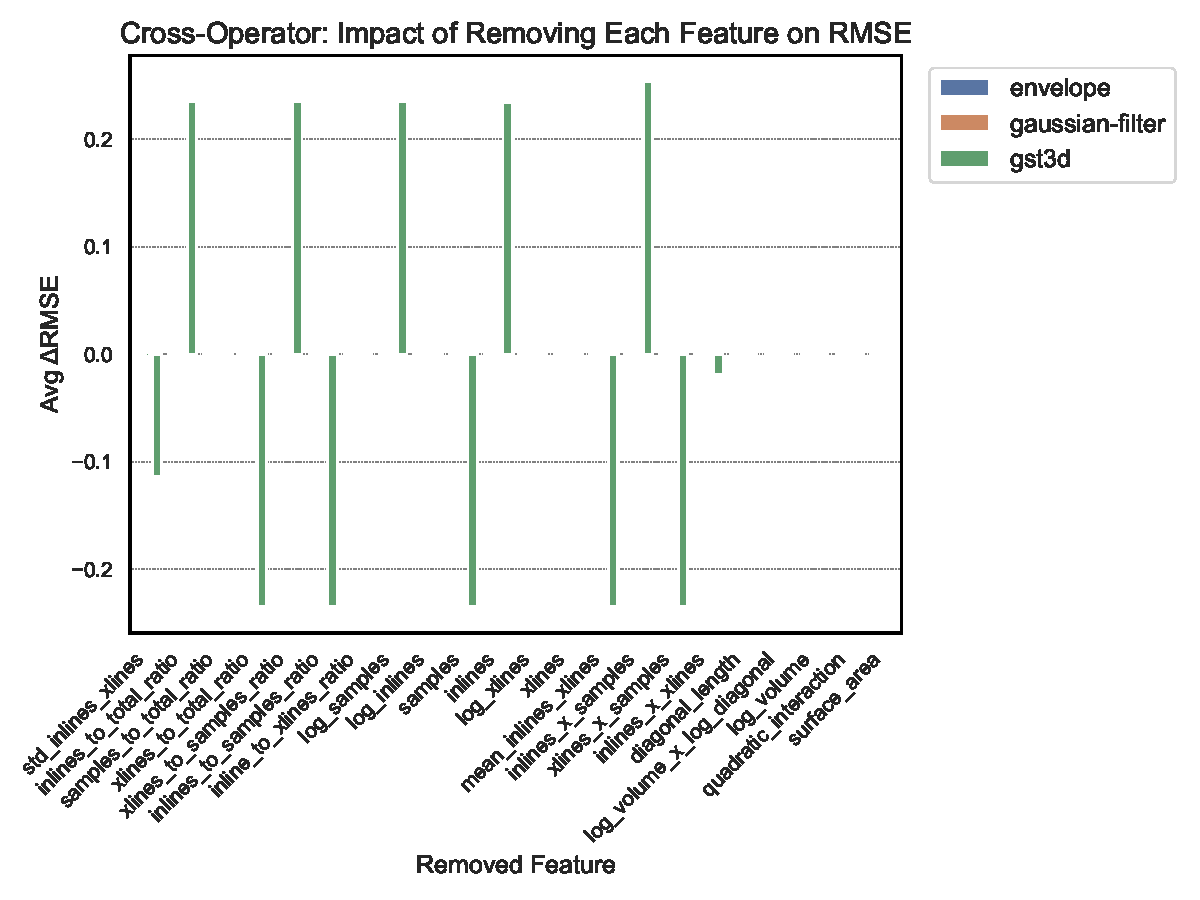
\includegraphics[width=\textwidth]{assets/images/05/feature_impact}
        \caption{Average \ac{RMSE} change per feature removal.
        Smaller bars indicate minimal impact.}
    \end{subfigure}
    \hfill
    \begin{subfigure}[t]{0.49\textwidth}
        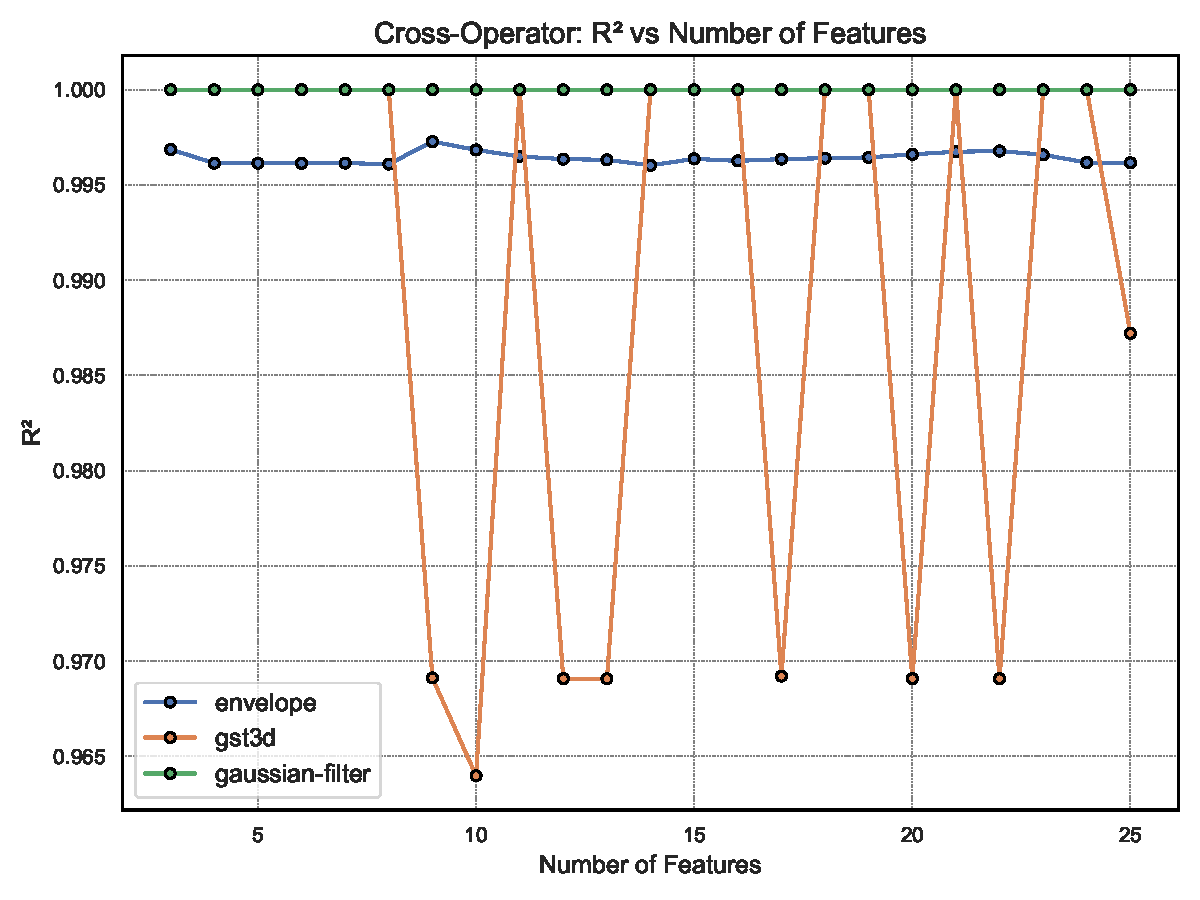
\includegraphics[width=\textwidth]{assets/images/05/cross_feature_selection_r2}
        \caption{$R^2$ changes during progressive feature removal across all operators.
        Volume stands out as indispensable.}
    \end{subfigure}
    \caption{Feature-removal impacts.
        Volume consistently emerges as the most critical input, whereas removing others typically yields negligible performance changes.
        \EB{Para argumentar que o volume é feature mais importante, não seria necessário mostrar que a remoção dela reduz o desempenho dos modelos?}
        \label{fig:feature_selection_overview_part1}
    }
\end{figure*}

Figure~\ref{fig:feature_selection_overview_part2} extends the analysis to residual-distribution metrics.
In particular, part~(b) shows that any small spikes in the residual curves do not substantially alter the final predictive reliability.
Hence, even simplified models (volume plus one or two shape parameters) are nearly as accurate as the full 25-feature configurations.

\begin{figure*}[htbp]
    \centering
    \begin{subfigure}[t]{0.49\textwidth}
        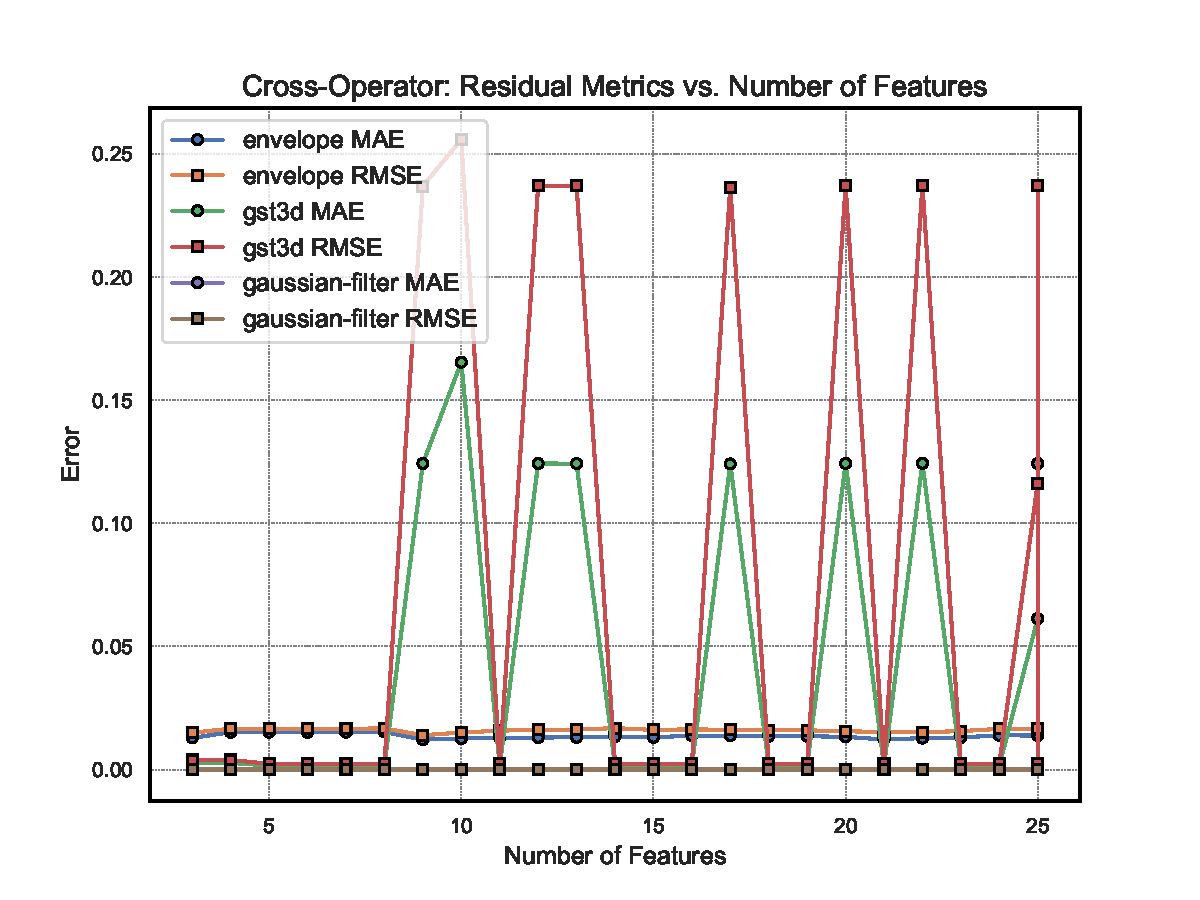
\includegraphics[width=\textwidth]{assets/images/05/residual_metrics_by_number_of_features}
        \caption{Residual-based metrics vs.\ number of features.
        Most fluctuations are minor.}
    \end{subfigure}
    \hfill
    \begin{subfigure}[t]{0.49\textwidth}
        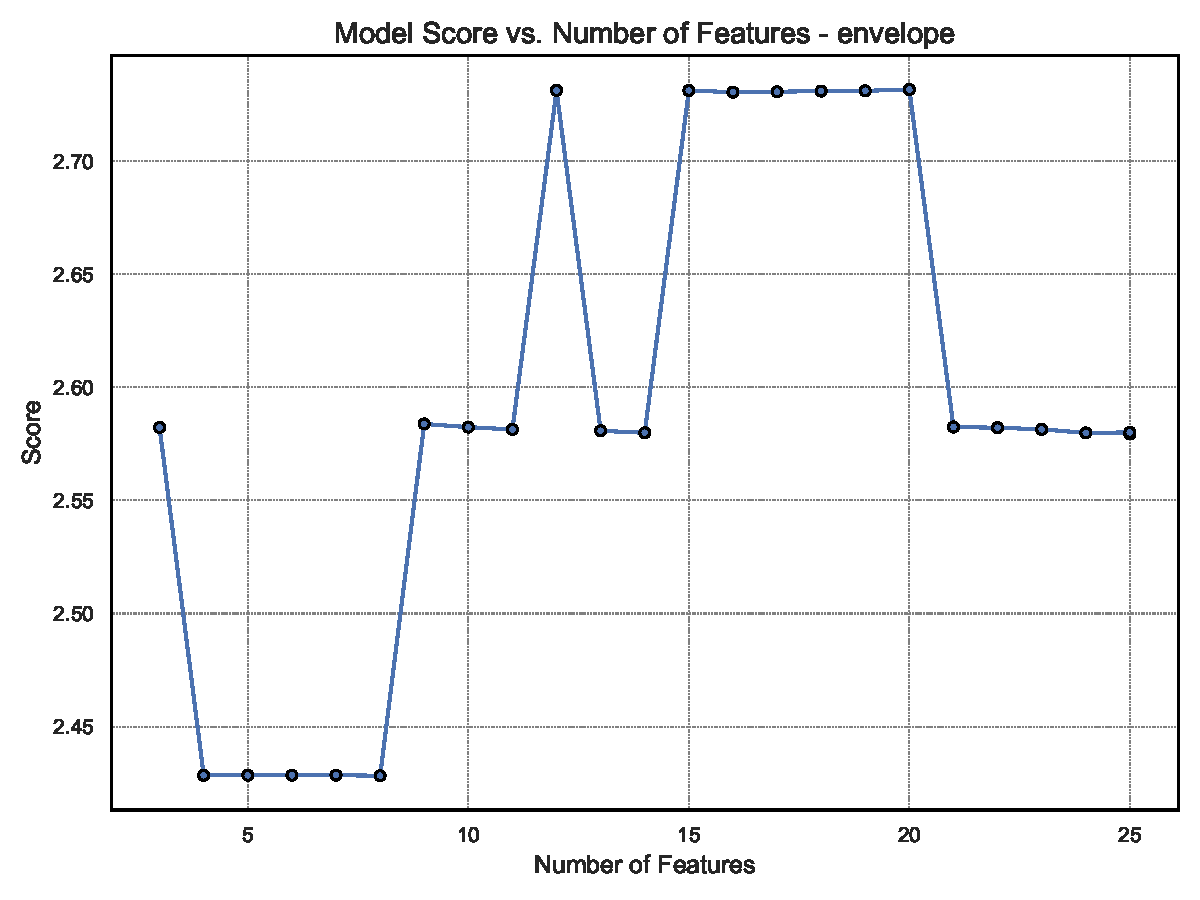
\includegraphics[width=\textwidth]{assets/images/05/score_by_number_of_features_envelope}
        \caption{Envelope example: overall “score” across successive feature removals.
        Scores remain stable or slightly improve.}
    \end{subfigure}
    \caption{Residual and score patterns under feature removal.
    Even with fewer predictors, model performance remains robust.}
    \label{fig:feature_selection_overview_part2}
\end{figure*}

\subsection{Operator-Specific Breakdown}
\label{subsec:operator-specific-breakdown}

Figures~\ref{fig:feature_impact_operator_subplots} and~\ref{fig:residual_metrics_by_number_of_features_operator_subplots} provide per-operator plots of the incremental feature-importance measurements.
The Envelope plots confirm that volume alone can achieve a \ac{RMSE} as low as 0.015.
Gaussian Filter achieves a \ac{RMSE} near \(2\times10^{-5}\) with only volume.
\ac{GST3D} benefits marginally from including another parameter (e.g., diagonal length), but dropping everything except \EBADD{the} volume \EBADD{efature} still yields strong $R^2 \approx 0.9999$ in many runs.

\begin{figure*}[htbp]
    \centering
    \begin{subfigure}[t]{0.32\textwidth}
        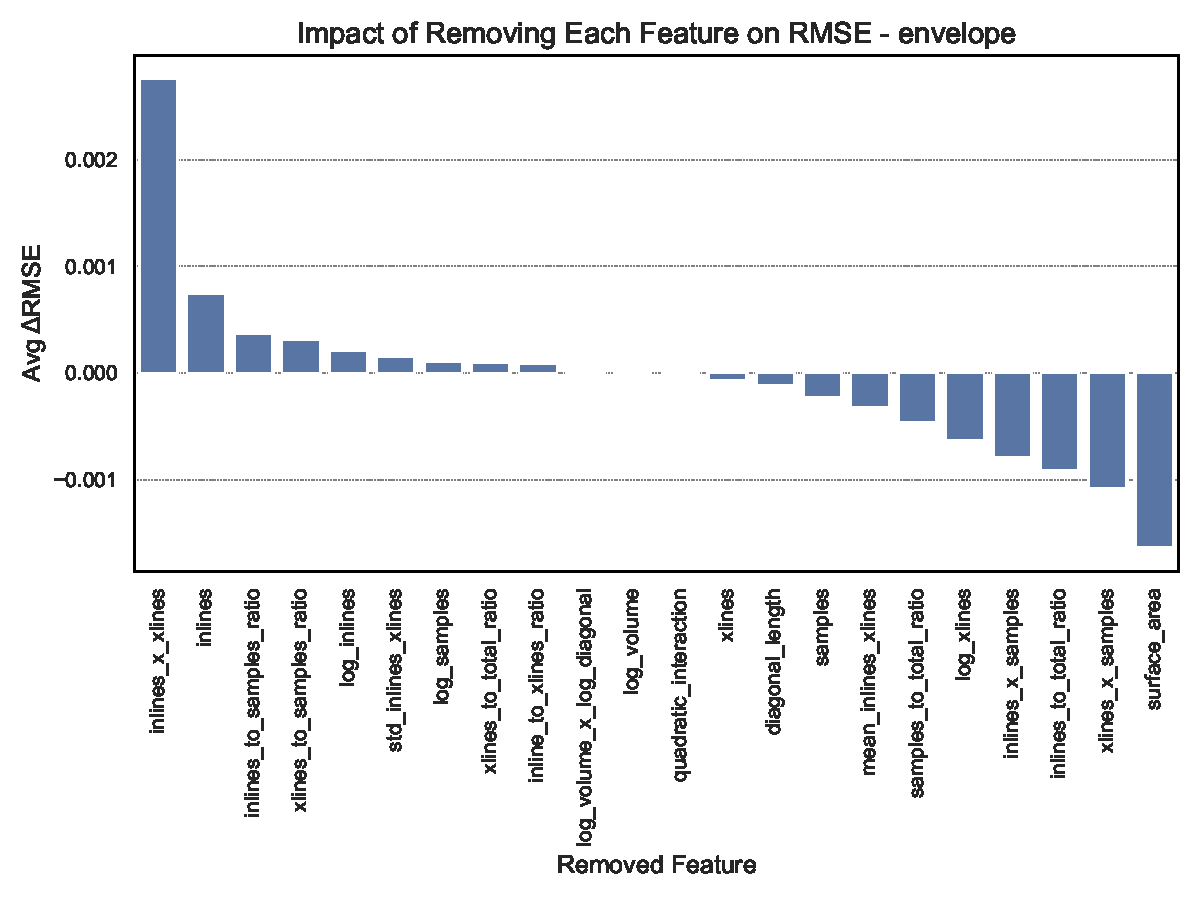
\includegraphics[width=\textwidth]{assets/images/05/feature_impact_envelope}
        \caption{Envelope}
    \end{subfigure}
    \hfill
    \begin{subfigure}[t]{0.32\textwidth}
        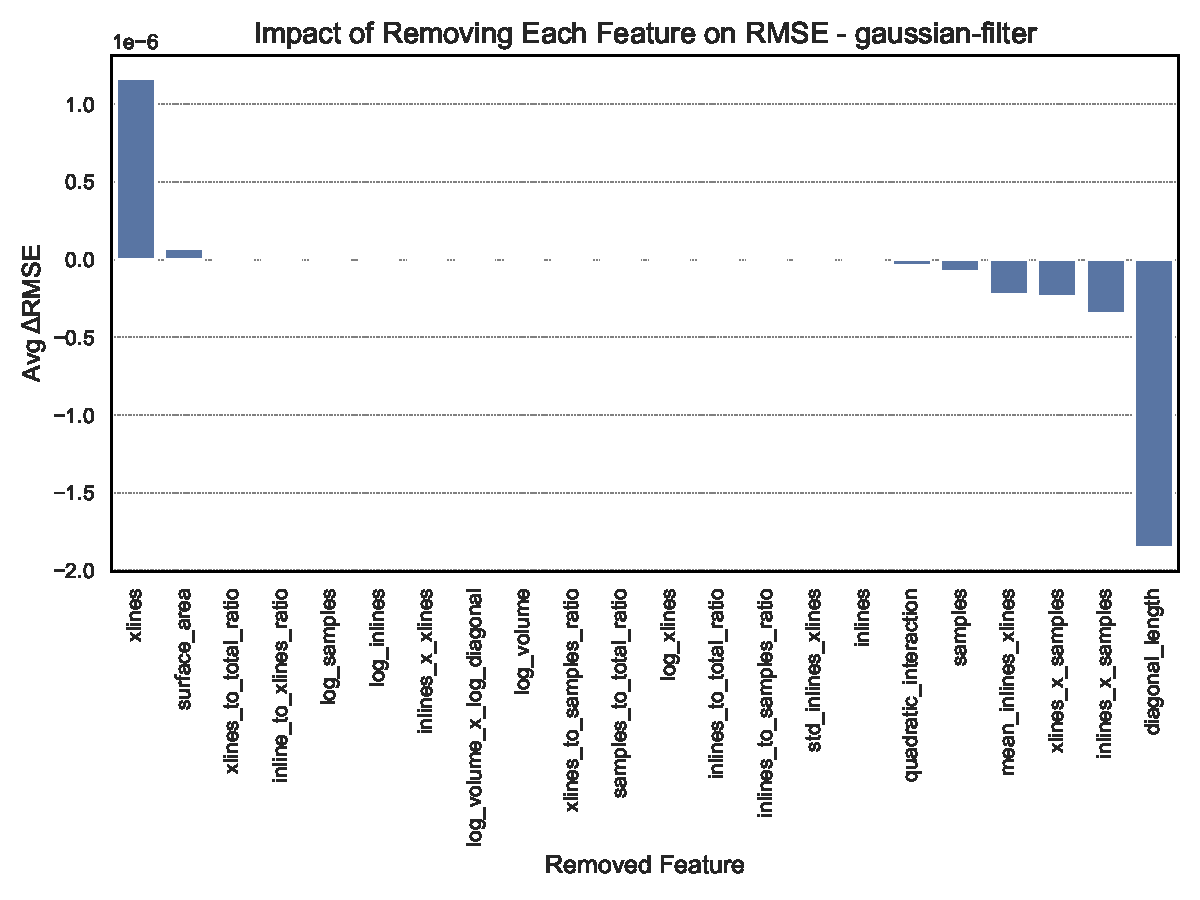
\includegraphics[width=\textwidth]{assets/images/05/feature_impact_gaussian-filter}
        \caption{Gaussian Filter}
    \end{subfigure}
    \hfill
    \begin{subfigure}[t]{0.32\textwidth}
        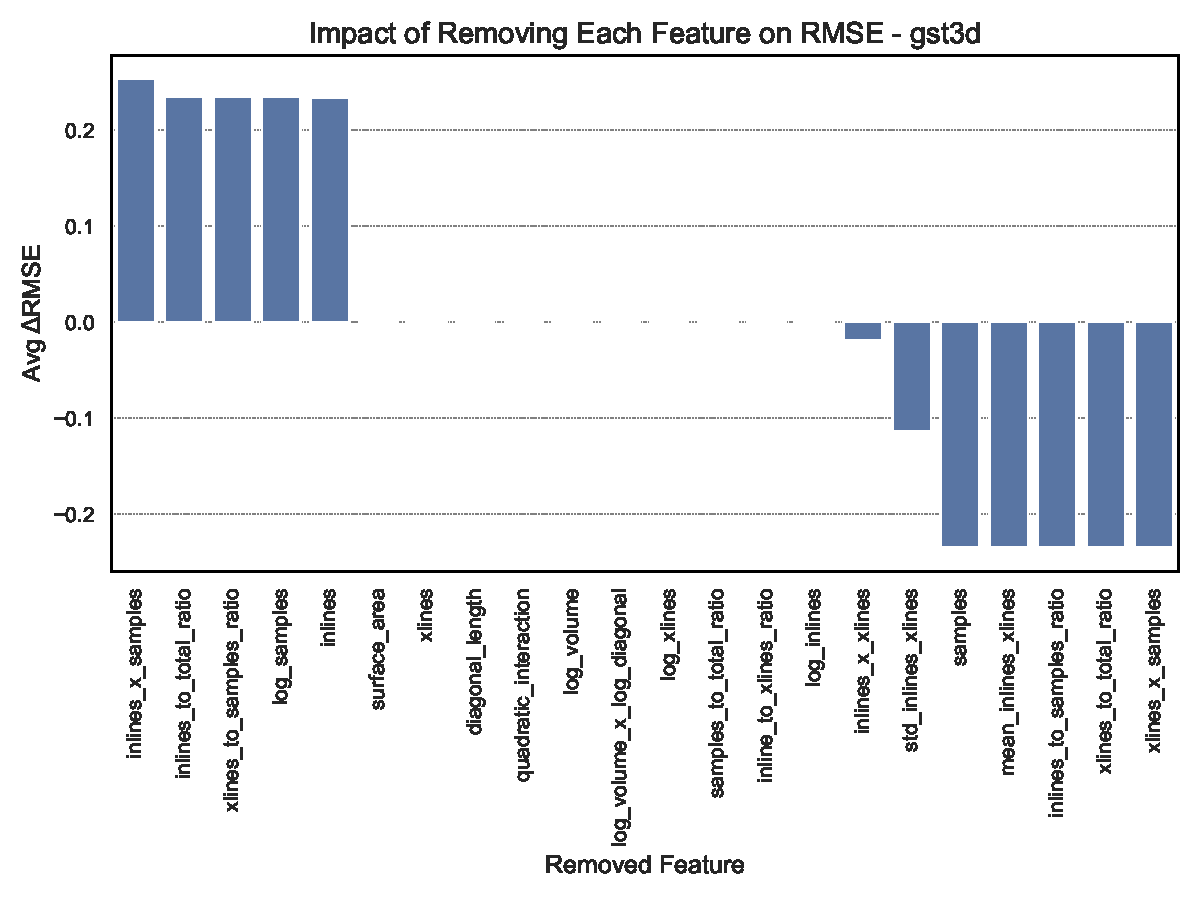
\includegraphics[width=\textwidth]{assets/images/05/feature_impact_gst3d}
        \caption{\ac{GST3D}}
    \end{subfigure}
    \caption{Feature-removal impact by operator.
        Bars represent the increase in \ac{RMSE} (or other metrics) upon discarding each feature.
        Volume is consistently the most essential.
        \EB{Que tal usar "Number of features removed" em vez de "Number of features" no eixo-x dos gráficos?}
        \EB{BTW, talvez fique melhor usar o mesmo eixo-y (mesmo intervalo no eixo-y) nos três gráficos.}
        \label{fig:feature_impact_operator_subplots}
    }
\end{figure*}

\begin{figure*}[htbp]
    \centering
    \begin{subfigure}[t]{0.32\textwidth}
        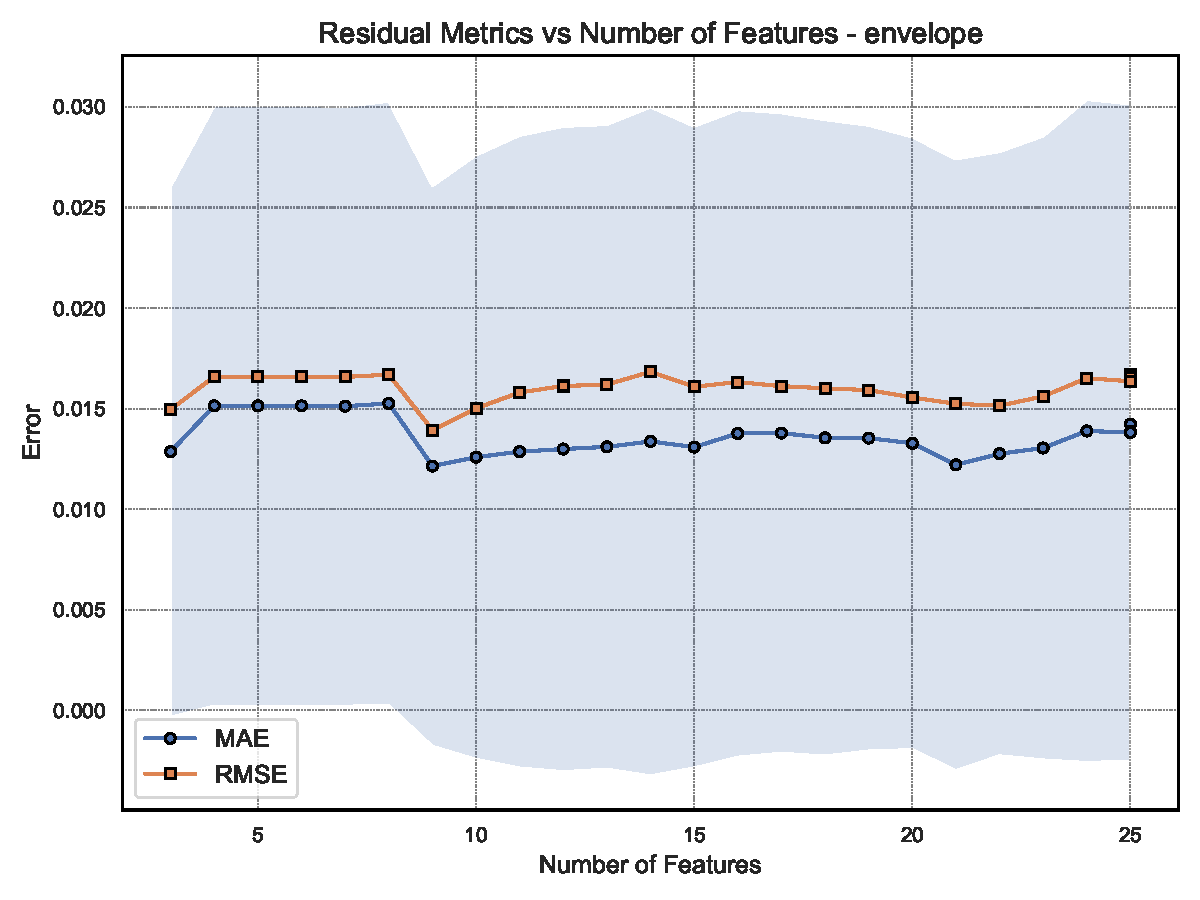
\includegraphics[width=\textwidth]{assets/images/05/residual_metrics_by_number_of_features_envelope}
        \caption{Envelope}
    \end{subfigure}
    \hfill
    \begin{subfigure}[t]{0.32\textwidth}
        \includegraphics[width=\textwidth]{assets/images/05/residual_metrics_by_number_of_features_gaussian-filter}
        \caption{Gaussian Filter}
    \end{subfigure}
    \hfill
    \begin{subfigure}[t]{0.32\textwidth}
        \includegraphics[width=\textwidth]{assets/images/05/residual_metrics_by_number_of_features_gst3d}
        \caption{\ac{GST3D}}
    \end{subfigure}
    \caption{Residual metrics versus number of features, split by operator.
    Envelope and Gaussian Filter are especially insensitive to feature reductions.
    \ac{GST3D} shows slightly larger performance dips when discarding non-volume inputs.}
    \label{fig:residual_metrics_by_number_of_features_operator_subplots}
\end{figure*}

\subsection{Summary of Findings}
\label{subsec:feature-selection-summary}

Collectively, these results support the conclusion that volume alone explains most memory usage variance in the tested seismic operators.
Limited improvements arise from including additional geometric attributes, yet the gain is usually minor.
Volume consistently appears in the top rank when applying \emph{SelectKBest} or other scoring schemes.
This aligns with earlier evidence of near-linear volume scaling (Section~\ref{sec:pmc-results-memory-and-execution-time-profiling}).

Practitioners seeking a lightweight memory-usage estimator can therefore rely on volume as the central input feature.
The next section investigate further data reduction (Section~\ref{sec:pmc-results-data-reduction-studies}) to refine the broader performance picture.
% like we did on feature selection, we tried to remove the amount of samples while testing the models. What we did was basically remove the "mean". So, we looked at the volume, kept the extremas, and removed (uniformly) the "middle"
% charts assets/images/05/cross_data_reduction_rmse.pdf and residual_metrics_by_sample_size.pdf show that the performance decreases. We can see that the RMSE increases, and the other metrics also increase. This is expected, since we are removing samples
% chart assets/images/05/metrics_evolution_by_sample_size.pdf show this as an overview by comparing all metrics in a facet for all operators
% charts assets/images/05/residual_metrics_by_sample_size_envelope.pdf, assets/images/05/residual_metrics_by_sample_size_gaussian-filter.pdf, and assets/images/05/residual_metrics_by_sample_size_gst3d.pdf show that the error metrics increase both in variability, as well as size, when we reduce the number of samples. We can see that it kepts some sort of stable until ~30 samples, and then it starts to increase
% charts assets/images/05/metrics_evolution_by_sample_size_envelope.pdf, assets/images/05/metrics_evolution_by_sample_size_gaussian-filter.pdf, and assets/images/05/metrics_evolution_by_sample_size_gst3d.pdf show all the metrics in a facet for each operator, showing that the error metrics increase when we reduce the number of samples
% charts assets/images/05/score_by_sample_size_envelope.pdf, assets/images/05/score_by_sample_size_gaussian-filter.pdf, and assets/images/05/score_by_sample_size_gst3d.pdf show the score of the models when we reduce the number of samples. We can see that the score decreases as we reduce the number of samples. But we also see that until ~30 it decreases slightly
% as we can see, we have a sweet spot close to 30

\section{Data Reduction Studies}
\label{sec:pmc-results-data-reduction-studies}

\EB{Acho que seria bom usar um título mais específico. Algo como: "Training Set Size", "Training Set Reduction Studies", "Impact of training set size"...}

This section discusses how predictive accuracy changes when the training dataset is subsampled, thus reducing the total number of configurations.
The aim is to identify whether smaller subsets of shape–memory measurements can still produce reliable models.
Specifically, experiments removed “middle-range” samples of the volume dimension (or shape parameters more broadly), keeping the smallest and largest volumes, while uniformly discarding intermediate sizes.
Both Envelope and \ac{GST3D} used the best models identified (Gradient Boosting and Decision Tree, respectively), while Gaussian Filter used Linear Regression.

\EB{Esta seção é bem interessante e importante. No entanto, a decisão de usar volumes pequenos e grandes em vez de pequenos e médios me pareceu arbitrária. Em tese, seria melhor usar pequenos e médios, já que o custo de coletar estes dados é menor.}

\subsection{Subsampling Strategy and Motivation}
\label{subsec:data-reduction-strategy-and-motivation}

The data-reduction procedure systematically excludes shape configurations from the central volume interval, retaining the extremes that often yield the highest or lowest memory usage.
By gradually lowering the sample count (\(N\)), it is possible to observe how model performance deteriorates or remains stable.
Figures~\ref{fig:cross_data_reduction_and_residual}--\ref{fig:metrics_evolution_sample_size_operators} present the overall results.
Figure~\ref{fig:cross_data_reduction_and_residual}(a) plots the \ac{RMSE} as a function of sample size, while part~(b) shows how residual-based metrics evolve.
All three operators suffer performance degradation under severe reductions, but moderate cutbacks can still yield acceptable accuracy.

\begin{figure*}[htbp]
    \centering
    \begin{subfigure}[t]{0.49\textwidth}
        \includegraphics[width=\textwidth]{assets/images/05/cross_data_reduction_rmse}
        \caption{\ac{RMSE} across Envelope, \ac{GST3D}, and Gaussian Filter as sample size decreases.
            A smooth upward trend reflects the increasing difficulty of fitting with fewer examples.
            \EB{Por que escolheu o RMSE em vez do outro score?}
        }
    \end{subfigure}
    \hfill
    \begin{subfigure}[t]{0.49\textwidth}
        \includegraphics[width=\textwidth]{assets/images/05/residual_metrics_by_sample_size}
        \caption{Residual metrics also climb with smaller datasets.
        Minimal sets (\(<20\) samples) show large spikes, indicating insufficient coverage of intermediate volumes.}
    \end{subfigure}
    \caption{Data-reduction effects, viewed globally for all operators.
        Reducing the training set drives up errors and variability.
        \EB{Estes dois gráficos são bem parecidos. Faz sentido manter os dois. Talvez o da esquerda já seja suficiente.}
        \label{fig:cross_data_reduction_and_residual}
    }
\end{figure*}

\subsection{Operator-Wise Performance Trends}
\label{subsec:operator-wise-sample-size-analysis}

Figures~\ref{fig:residual_metrics_by_sample_size_operators}--\ref{fig:metrics_evolution_sample_size_operators} elaborate on each operator individually.
When sample sizes fall below roughly 30, \ac{RMSE}, \ac{MAE}, and residual variance begin to rise more sharply.
This pattern is consistent with the notion that “filling in” the middle range of volumes is essential for maintaining a robust regression fit.
However, moderately pruned datasets (e.g., 40–50 samples) still achieve respectable $R^2 > 0.98$ in most cases, as verified by the CSV results in Table~\ref{tab:data_reduction_summary}. \EB{Referência quebrada}

\begin{figure*}[htbp]
    \centering
    \begin{subfigure}[t]{0.32\textwidth}
        \includegraphics[width=\textwidth]{assets/images/05/residual_metrics_by_sample_size_envelope}
        \caption{Envelope}
    \end{subfigure}
    \hfill
    \begin{subfigure}[t]{0.32\textwidth}
        \includegraphics[width=\textwidth]{assets/images/05/residual_metrics_by_sample_size_gaussian-filter}
        \caption{Gaussian Filter}
    \end{subfigure}
    \hfill
    \begin{subfigure}[t]{0.32\textwidth}
        \includegraphics[width=\textwidth]{assets/images/05/residual_metrics_by_sample_size_gst3d}
        \caption{\ac{GST3D}}
    \end{subfigure}
    \caption{Residual-based metrics per operator as sample size diminishes.
    Error bars reflect increasing variability at smaller dataset sizes.}
    \label{fig:residual_metrics_by_sample_size_operators}
\end{figure*}

\begin{figure*}[htbp]
    \centering
    \begin{subfigure}[t]{0.32\textwidth}
        \includegraphics[width=\textwidth]{assets/images/05/metrics_evolution_by_sample_size_envelope}
        \caption{Envelope}
    \end{subfigure}
    \hfill
    \begin{subfigure}[t]{0.32\textwidth}
        \includegraphics[width=\textwidth]{assets/images/05/metrics_evolution_by_sample_size_gaussian-filter}
        \caption{Gaussian Filter}
    \end{subfigure}
    \hfill
    \begin{subfigure}[t]{0.32\textwidth}
        \includegraphics[width=\textwidth]{assets/images/05/metrics_evolution_by_sample_size_gst3d}
        \caption{\ac{GST3D}}
    \end{subfigure}
    \caption{All metrics tracked as sample sizes drop, plotted per operator.
        \ac{RMSE} and \ac{MAE} grow steadily, while $R^2$ and accuracy decline.}
    \label{fig:metrics_evolution_sample_size_operators}
\end{figure*}

\subsection{Score Comparisons and Sweet Spot Around 30 Samples}
\label{subsec:score-comparisons-and-sweet-spot}

Figures~\ref{fig:score_by_sample_size_operators}(a)–(c) plot the consolidated “score” metric described in Section~\ref{sec:pmc-results-model-performance-overview}.
All three operators see an inflection around 30–35 samples where model quality remains strong.
Below that threshold, the curves dip more significantly, reflecting the loss of mid-range volume coverage.
Above 40–50 samples, the gains saturate, and further additions of similar configurations do not yield major improvements.

\begin{figure*}[htbp]
    \centering
    \begin{subfigure}[t]{0.32\textwidth}
        \includegraphics[width=\textwidth]{assets/images/05/score_by_sample_size_envelope}
        \caption{Envelope}
    \end{subfigure}
    \hfill
    \begin{subfigure}[t]{0.32\textwidth}
        \includegraphics[width=\textwidth]{assets/images/05/score_by_sample_size_gaussian-filter}
        \caption{Gaussian Filter}
    \end{subfigure}
    \hfill
    \begin{subfigure}[t]{0.32\textwidth}
        \includegraphics[width=\textwidth]{assets/images/05/score_by_sample_size_gst3d}
        \caption{\ac{GST3D}}
    \end{subfigure}
    \caption{Model scores vs.\ sample size.
    Each operator shows a notable decline below \(\sim\)30 samples, marking a practical lower bound for training.}
    \label{fig:score_by_sample_size_operators}
\end{figure*}

Table~\ref{tab:data_reduction_summary} illustrates partial data from the CSV logs (see \texttt{envelope.csv}, \texttt{gaussian-filter.csv}, and \texttt{gst3d.csv}). 
\EB{Corrigir a Referência quebrada e a invasão de margem.}
It includes selected sample sizes and the resulting \ac{RMSE}, $R^2$, accuracy, and overall score.
Even moderate subsampling (34 or 42 samples, for instance) still achieves high $R^2$ for Envelope and Gaussian Filter.
\ac{GST3D} remains more sensitive, though a subset of 44 samples can deliver near-perfect accuracy.

\begin{table}[htbp]
    \centering
    \begin{tabular}{lccccc}
        \hline
        \textbf{Operator} & \textbf{\#Samples} & \textbf{\ac{RMSE}}    & \textbf{$R^2$} & \textbf{Accuracy} & \textbf{Score} \\
        \hline
        \multirow{3}{*}{\textbf{Envelope}}
        & 64                 & 0.0170                & 0.9959         & 0.8462            & 2.5789         \\
        & 34                 & 0.0217                & 0.9926         & 0.7143            & 2.3113         \\
        & 11                 & 0.2463                & 0.8805         & 0.3333            & 1.2155         \\
        \hline
        \multirow{3}{*}{\textbf{Gaussian Filter}}
        & 64                 & \(2.37\times10^{-5}\) & 0.9999999      & 1.0               & 2.9045         \\
        & 34                 & \(2.90\times10^{-5}\) & 0.9999998      & 1.0               & 2.9044         \\
        & 11                 & \(1.02\times10^{-4}\) & 0.9999997      & 1.0               & 2.9044         \\
        \hline
        \multirow{3}{*}{\textbf{\ac{GST3D}}}
        & 54                 & 0.2371                & 0.9691         & 0.7273            & 2.0478         \\
        & 29                 & 0.3689                & 0.9251         & 0.8333            & 2.0472         \\
        & 11                 & 1.1042                & 0.7684         & 0.0000            & -1.0768        \\
        \hline
    \end{tabular}
    \caption{Selected data-reduction results (largest, close to 30, smallest) for each operator.
    Subsets of around 30--40 samples retain robust accuracy, while very small sets
        (e.g., 11) cause steep performance declines, especially for \ac{GST3D}.}
    \label{tab:data_reduction_small_vs_medium_vs_large}
\end{table}

\subsection{Conclusions on Data Pruning}
\label{subsec:data-reduction-conclusions}

These experiments confirm that seismic-memory models require at least 30 samples to maintain stable performance, primarily to capture mid-scale volumes.
Envelope and Gaussian Filter remain accurate even with moderate data pruning, while \ac{GST3D} is somewhat more sensitive due to its heavier internal complexity.
Still, collecting 30–40 shape configurations seems sufficient for building robust predictive models without incurring excessive data-gathering overhead.
Subsequent sections integrate these findings with the feature-selection insights to propose minimal yet effective training strategies for real-world \ac{HPC} applications.
\section{Conclusion}
\label{sec:pmc-conclusion}

This chapter explored the relationship between seismic input shapes and operator-specific memory consumption, focusing on three major processing routines—Envelope, \ac{GST3D}, and Gaussian Filter—and detailed how varying sample sizes, selected features, and modeling pipelines affect predictive accuracy.
Several salient findings emerged:

\begin{itemize}
    \item \textbf{Linear Volume Dependence and Operator Sensitivity.}
    All operators demonstrated a near-linear escalation in peak \ac{RAM} usage with respect to total input volume (\( \text{inlines} \times \text{xlines} \times \text{samples} \)).
    \ac{GST3D} remained the most sensitive, displaying a steeper volume-based slope compared to Envelope and Gaussian Filter.
    Envelope and Gaussian Filter, by contrast, showed comparatively gentler linear relationships, suggesting that their computational kernels rely less on large intermediate buffers.

    \item \textbf{Feature Selection and the Predominance of Volume.}
    Systematic removal of shape-derived features (e.g., diagonal length, surface area, ratio transformations) underscored that \emph{volume} alone captures most of the variance in peak memory usage.
    Even advanced transformations (logarithmic or polynomial terms) contributed only marginal improvements once volume was included.
    \ac{GST3D} occasionally benefited from additional parameters (e.g., diagonal length), but not enough to outweigh the straightforward predictive power of volume.

    \item \textbf{Model Performance and Robustness.}
    Across nine regression approaches, simpler or regularized methods—like \ac{Linear Regression}, Elastic Net, and decision-tree ensembles—performed well, achieving \(R^2 \approx 0.99\) or higher in many configurations.
    Specifically:
    \begin{itemize}
        \item \textbf{Envelope}: Gradient Boosting offered top-level accuracy, though multiple models clustered in the same performance range.
        \item \textbf{\ac{GST3D}}: Decision Trees (and some ensemble variants) captured memory usage reliably but exhibited greater sensitivity to missing data in the mid-volume range.
        \item \textbf{Gaussian Filter}: \ac{Linear Regression} proved sufficient, reinforcing that this operator’s memory footprint aligns closely with volume.
    \end{itemize}
    All methods exhibited mild to moderate right-skew in their residual distributions, yet \ac{RMSE} and \ac{MAE} remained low once mid- and upper-bound volumes were adequately represented.

    \item \textbf{Subsampling and Data Requirements.}
    Pruning the dataset to 30–40 shape configurations preserved high $R^2$ values, indicating that modest sampling—particularly anchored at small and large volumes—enables accurate modeling.
    \ac{GST3D} showed slightly larger degradation at smaller sample counts, reflecting its more complex intermediate data allocations.
    By contrast, Envelope and Gaussian Filter sustained robust predictions with moderate data reduction.
\end{itemize}

Overall, Chapter~\ref{sec:pmc-results} establishes that:
\begin{enumerate}
    \item \emph{Volume is the primary explanatory feature} for predicting peak memory usage, with additional variables offering only minor gains.
    \item Simple or linear-in-spirit regressors often suffice to model Envelope and Gaussian Filter, while \ac{GST3D} can benefit from tree-based methods if data coverage in the mid-volume range is adequate.
    \item A sample size of approximately 30–40 shape configurations provides a practical lower bound for stable memory prediction, making data collection efforts more tractable for real-world \ac{HPC} scenarios.
\end{enumerate}

With these findings, we have a clearer framework for implementing memory-aware chunking strategies: one can rely on volume-based models (potentially augmented by minimal shape features) and still maintain accurate peak \ac{RAM} \EBADD{consumption} estimates, even with relatively small training sets.
The subsequent chapter applies these insights to optimize data-parallel chunking and scheduling decisions for large-scale seismic workloads.
    \chapter{Improving Data Parallelism using Memory-Aware Chunking}
\label{ch:improving-data-parallelism-using-memory-aware-chunking}


\section{Introduction}
\label{sec:mac-introduction}

\DFTODO{Explicar sobre o uso do paralelismo de dados}
\DFTODO{Explicar sobre a importância de se ter um bom balanceamento de carga e como isso pode ser feito.}
\DFTODO{Explicar sobre o uso de chunking para o balanceamento de carga}
\DFTODO{Conectar a seção anterior, falando que é feito tentativa e erro pra definir o tamanho do chunk}
\DFTODO{Explicar sobre a natureza de algoritmos tensoriais e linkar com a sessão anterior que é possível prever o consumo de memória}


\section{Dask Auto-Chunking}
\label{sec:mac-dask-auto-chunking}

\DFTODO{Explicar como o auto-chunking do dask funciona e suas limitações}


\section{Memory-Aware Chunking}
\label{sec:mac-memory-aware-chunking}

\DFTODO{Explicar sobre a proposta de chunking baseado no consumo de memória}


\section{Materials and Methods}
\label{sec:mac-materials-methods}

\DFTODO{Explicar sobre o setup do experimento de um ponto de vista de hardware}
\DFTODO{Explicar sobre o setup do experimento de um ponto de vista de software}
\DFTODO{Descrever o fluxo de execução do experimento}
\DFTODO{Explicar como foi feita a configuração do cluster Dask}
\DFTODO{Descrever os experimentos com chunks diferentes para demonstrar as limitações do Dask auto-chunking}
\DFTODO{Descrever a geração de dados, linkando com a sessão anterior}
\DFTODO{Descrever os algoritmos, linkando com a sessão anterior}
\DFTODO{Descrever as métricas coletadas: tempo de execução, uso máximo de memória, overhead de escalonamento, número de chunks, relação chunk-to-worker, temanho relativo do chunk}
\DFTODO{Descrever as técnicas utilizadas para analisar os dados}
\DFTODO{Linkar com o código fonte}


\section{Experimental Results}
\label{sec:mac-experimental-results}

\DFTODO{Descrever como diferentes formatos de chunk afetam o desempenho}
\DFTODO{Demonstrar e comparar o Memory-Aware Chunking com o Auto-Chunking do Dask}
\DFTODO{Demonstrar e descrever o previsor de melhor tamanho de chunk que foi desenvolvido com base nos resultados}


\section{Conclusion}
\label{sec:mac-conclusion}

\DFTODO{Concluir sobre a importância de se ter um bom balanceamento de carga}
\DFTODO{Explicar e concluir sobre a possibilidade de encontrar o melhor tamanho de chunk baseado no consnumo estimado de memória}
\DFTODO{Discutir as complexidades e próximos passos para integrar facilmente com o Dask}


    \chapter{Conclusion}
\label{ch:conclusion}

\DFTODO{Organizar e escrever a conclusão}

    \bibliographystyle{plain}
    \bibliography{bibliography}

% \appendix
% \chapter{Anexo 1}
% \chapter{Anexo 2}

\end{document}